\documentclass[]{krantz}
\usepackage{lmodern}
\usepackage{amssymb,amsmath}
\usepackage{ifxetex,ifluatex}
\usepackage{fixltx2e} % provides \textsubscript
\ifnum 0\ifxetex 1\fi\ifluatex 1\fi=0 % if pdftex
  \usepackage[T1]{fontenc}
  \usepackage[utf8]{inputenc}
\else % if luatex or xelatex
  \ifxetex
    \usepackage{mathspec}
  \else
    \usepackage{fontspec}
  \fi
  \defaultfontfeatures{Ligatures=TeX,Scale=MatchLowercase}
\fi
% use upquote if available, for straight quotes in verbatim environments
\IfFileExists{upquote.sty}{\usepackage{upquote}}{}
% use microtype if available
\IfFileExists{microtype.sty}{%
\usepackage{microtype}
\UseMicrotypeSet[protrusion]{basicmath} % disable protrusion for tt fonts
}{}
\usepackage[margin=1in]{geometry}
\usepackage{hyperref}
\PassOptionsToPackage{usenames,dvipsnames}{color} % color is loaded by hyperref
\hypersetup{unicode=true,
            pdftitle={Predictive Models: Visualisation, Exploration and Explanation},
            pdfauthor={Przemyslaw Biecek and Tomasz Burzykowski},
            colorlinks=true,
            linkcolor=Maroon,
            citecolor=Blue,
            urlcolor=Blue,
            breaklinks=true}
\urlstyle{same}  % don't use monospace font for urls
\usepackage{natbib}
\bibliographystyle{apalike}
\usepackage{color}
\usepackage{fancyvrb}
\newcommand{\VerbBar}{|}
\newcommand{\VERB}{\Verb[commandchars=\\\{\}]}
\DefineVerbatimEnvironment{Highlighting}{Verbatim}{commandchars=\\\{\}}
% Add ',fontsize=\small' for more characters per line
\usepackage{framed}
\definecolor{shadecolor}{RGB}{248,248,248}
\newenvironment{Shaded}{\begin{snugshade}}{\end{snugshade}}
\newcommand{\AlertTok}[1]{\textcolor[rgb]{0.94,0.16,0.16}{#1}}
\newcommand{\AnnotationTok}[1]{\textcolor[rgb]{0.56,0.35,0.01}{\textbf{\textit{#1}}}}
\newcommand{\AttributeTok}[1]{\textcolor[rgb]{0.77,0.63,0.00}{#1}}
\newcommand{\BaseNTok}[1]{\textcolor[rgb]{0.00,0.00,0.81}{#1}}
\newcommand{\BuiltInTok}[1]{#1}
\newcommand{\CharTok}[1]{\textcolor[rgb]{0.31,0.60,0.02}{#1}}
\newcommand{\CommentTok}[1]{\textcolor[rgb]{0.56,0.35,0.01}{\textit{#1}}}
\newcommand{\CommentVarTok}[1]{\textcolor[rgb]{0.56,0.35,0.01}{\textbf{\textit{#1}}}}
\newcommand{\ConstantTok}[1]{\textcolor[rgb]{0.00,0.00,0.00}{#1}}
\newcommand{\ControlFlowTok}[1]{\textcolor[rgb]{0.13,0.29,0.53}{\textbf{#1}}}
\newcommand{\DataTypeTok}[1]{\textcolor[rgb]{0.13,0.29,0.53}{#1}}
\newcommand{\DecValTok}[1]{\textcolor[rgb]{0.00,0.00,0.81}{#1}}
\newcommand{\DocumentationTok}[1]{\textcolor[rgb]{0.56,0.35,0.01}{\textbf{\textit{#1}}}}
\newcommand{\ErrorTok}[1]{\textcolor[rgb]{0.64,0.00,0.00}{\textbf{#1}}}
\newcommand{\ExtensionTok}[1]{#1}
\newcommand{\FloatTok}[1]{\textcolor[rgb]{0.00,0.00,0.81}{#1}}
\newcommand{\FunctionTok}[1]{\textcolor[rgb]{0.00,0.00,0.00}{#1}}
\newcommand{\ImportTok}[1]{#1}
\newcommand{\InformationTok}[1]{\textcolor[rgb]{0.56,0.35,0.01}{\textbf{\textit{#1}}}}
\newcommand{\KeywordTok}[1]{\textcolor[rgb]{0.13,0.29,0.53}{\textbf{#1}}}
\newcommand{\NormalTok}[1]{#1}
\newcommand{\OperatorTok}[1]{\textcolor[rgb]{0.81,0.36,0.00}{\textbf{#1}}}
\newcommand{\OtherTok}[1]{\textcolor[rgb]{0.56,0.35,0.01}{#1}}
\newcommand{\PreprocessorTok}[1]{\textcolor[rgb]{0.56,0.35,0.01}{\textit{#1}}}
\newcommand{\RegionMarkerTok}[1]{#1}
\newcommand{\SpecialCharTok}[1]{\textcolor[rgb]{0.00,0.00,0.00}{#1}}
\newcommand{\SpecialStringTok}[1]{\textcolor[rgb]{0.31,0.60,0.02}{#1}}
\newcommand{\StringTok}[1]{\textcolor[rgb]{0.31,0.60,0.02}{#1}}
\newcommand{\VariableTok}[1]{\textcolor[rgb]{0.00,0.00,0.00}{#1}}
\newcommand{\VerbatimStringTok}[1]{\textcolor[rgb]{0.31,0.60,0.02}{#1}}
\newcommand{\WarningTok}[1]{\textcolor[rgb]{0.56,0.35,0.01}{\textbf{\textit{#1}}}}
\usepackage{longtable,booktabs}
\usepackage{graphicx,grffile}
\makeatletter
\def\maxwidth{\ifdim\Gin@nat@width>\linewidth\linewidth\else\Gin@nat@width\fi}
\def\maxheight{\ifdim\Gin@nat@height>\textheight\textheight\else\Gin@nat@height\fi}
\makeatother
% Scale images if necessary, so that they will not overflow the page
% margins by default, and it is still possible to overwrite the defaults
% using explicit options in \includegraphics[width, height, ...]{}
\setkeys{Gin}{width=\maxwidth,height=\maxheight,keepaspectratio}
\IfFileExists{parskip.sty}{%
\usepackage{parskip}
}{% else
\setlength{\parindent}{0pt}
\setlength{\parskip}{6pt plus 2pt minus 1pt}
}
\setlength{\emergencystretch}{3em}  % prevent overfull lines
\providecommand{\tightlist}{%
  \setlength{\itemsep}{0pt}\setlength{\parskip}{0pt}}
\setcounter{secnumdepth}{5}
% Redefines (sub)paragraphs to behave more like sections
\ifx\paragraph\undefined\else
\let\oldparagraph\paragraph
\renewcommand{\paragraph}[1]{\oldparagraph{#1}\mbox{}}
\fi
\ifx\subparagraph\undefined\else
\let\oldsubparagraph\subparagraph
\renewcommand{\subparagraph}[1]{\oldsubparagraph{#1}\mbox{}}
\fi

%%% Use protect on footnotes to avoid problems with footnotes in titles
\let\rmarkdownfootnote\footnote%
\def\footnote{\protect\rmarkdownfootnote}

%%% Change title format to be more compact
\usepackage{titling}

% Create subtitle command for use in maketitle
\newcommand{\subtitle}[1]{
  \posttitle{
    \begin{center}\large#1\end{center}
    }
}

\setlength{\droptitle}{-2em}

  \title{Predictive Models: Visualisation, Exploration and Explanation}
    \pretitle{\vspace{\droptitle}\centering\huge}
  \posttitle{\par}
  \subtitle{With examples in R and Python}
  \author{Przemyslaw Biecek and Tomasz Burzykowski}
    \preauthor{\centering\large\emph}
  \postauthor{\par}
      \predate{\centering\large\emph}
  \postdate{\par}
    \date{2018-09-28}

\usepackage{booktabs}

\usepackage{amsthm}
\newtheorem{theorem}{Theorem}[section]
\newtheorem{lemma}{Lemma}[section]
\theoremstyle{definition}
\newtheorem{definition}{Definition}[section]
\newtheorem{corollary}{Corollary}[section]
\newtheorem{proposition}{Proposition}[section]
\theoremstyle{definition}
\newtheorem{example}{Example}[section]
\theoremstyle{definition}
\newtheorem{exercise}{Exercise}[section]
\theoremstyle{remark}
\newtheorem*{remark}{Remark}
\newtheorem*{solution}{Solution}
\begin{document}
\maketitle

{
\hypersetup{linkcolor=black}
\setcounter{tocdepth}{2}
\tableofcontents
}
\listoftables
\listoffigures
\hypertarget{introduction}{%
\section{Introduction}\label{introduction}}

Predictive models are used to automatically guess (statisticians would
say: estimate) one interesting variable based on other variables. Think
about prediction of sales based on historical data, prediction of risk
of heart disease based on patient characteristics, prediction of
political attitudes based on facebook comments.

Predictive models were constructed through the whole human history.
Think about Flooding of the Nile for example. More rigorous approach to
model construction may be attributed to the method of least squares,
published by Legendre in 1805, and by Gauss in 1809, more than two
centuries ago. Number of applications in economy, medicine, biology,
agriculture was growing. The term \emph{regression} was coined by
Francis Galton in 1886, initially was referring to biological
applications, today is used for various models that predict continues
variable. Prediction of nominal variables is called
\emph{classification}, and its beginning may be attributed to works of
Ronald Fisher in 1936.

During the last century we observed lot of developments in predictive
models like linear models, generalized models, regression and
classification trees, rule based models and many others. Developments in
mathematical foundations of predictive models were boosted by increasing
computational power of personal computers and availability of large
datasets. So called the era of big data.

Increasing demand on predictive models favour models that are elastic,
able to perform internally some feature engineering and leads to high
precision of predictions. Robust models are now created with ensembles
of models. Techniques like bagging, boosting or model stacking gather
hundreds or thousands of small model into a one super model. Large deep
neural models have over bilion of parameters.

There is a cost of this progress. Large models are opaque, obscure, they
act like black boxes. On one hand, human is unable to understand how
thousands of coefficients affect the model response, one the another
hand the model itself may be threated as a trade secret. And the worst
part of this is that these models are not as good as we wish them to be.

Decieved by model performance, big names of model producer we tend to
believe that these black boxes are unerring oracles. The thruth is that
they are not. And we have more and more examples that model performance
deteriorate with time or is biased in some sense.

An overview of real problems with large black box models may be found in
an excellent book of Cathy O'Neil \citep{ONeil} on in her TED Talk
,,\emph{The era of blind faith in big data must end}'`. Variouse
examples show how models that are opaque and unregulated lead to higher
discrimination of inequality. And there is more examples of such
problems, see ,,\emph{Google and the flu: how big data will help us make
gigantic mistakes}'`, ,,\emph{Report: IBM Watson delivered 'unsafe and
inaccurate' cancer recommendations}''.

Today the true bottleneck for predictive modelling is not the lack of
data, nor lack of computational power, nor lack of elastic models. It's
lack of tools for model validation, explorations and explanations of
model decisions.

In this book we present collection of methods that may be used for this
purpose. It is a very active area of research and for sure more methods
will be developed in this area. However here we present the mind-set,
key problems and methods that are used in model exploration.

\textbf{This book is about}

\begin{itemize}
\tightlist
\item
  We show how to determine features that affect model response for a
  selected observation. In this book you will find theory and examples
  that explains prediction level methods like break down plots, ceteris
  paribus profiles, Local model approximations or Shapley values.
\item
  We present techniques to examine fully trained Machine Learning models
  as a whole. In this book you will find theory and examples that
  explains model globally like Partial Dependency Plots, Variable
  Importance Plots and others.
\item
  We present charts that are used to present key information in a quick
  way.
\item
  We present tools and methods for model comparison.
\item
  We present example code snippets for R and python that show how to use
  described methods.
\end{itemize}

\textbf{This book is NOT about.}

\begin{itemize}
\tightlist
\item
  We do not focus on any specific model. Presented techniques are model
  agnostic and do not have any assumptions related to model structure.
\item
  We do not focus on the data exploration. There are very good books and
  techniques related to this, like R for Data Science
  \url{http://r4ds.had.co.nz/} or TODO
\item
  We do not focus on the process of model building. There are also very
  good books about this, see An Introduction to Statistical Learning by
  Gareth James, Daniela Witten, Trevor Hastie and Robert Tibshirani
  \url{http://www-bcf.usc.edu/~gareth/ISL/} or TODO
\item
  We do not focus on particular tools for model building, see Applied
  Predictive Modeling By Max Kuhn and Kjell Johnson
  \url{http://appliedpredictivemodeling.com/}
\end{itemize}

\textbf{This book has following structure}

\begin{itemize}
\tightlist
\item
  In the Section 1 we introduce notation and vocabulary that will be
  used in this book. Same concepts have often different names in
  statistics and different in machine learning, thus show how to
  translate between these two worlds. In this section we also set
  expectations.
\item
  In the part \emph{Prediction level explainers} we present techniques
  for exploration and explanations single model predictions.
\item
  In the part \emph{Model level explainers} we present techniques for
  exploration and explanations model as a whole.
\end{itemize}

Every method for model exploration is described in a separate section.
In each such section you will find.

\begin{itemize}
\tightlist
\item
  Subsection \emph{Introduction}, that explains the goal of the method
  and the general idea behind this method.
\item
  Subsection \emph{The Algorithm}, that shows mathematical or
  computational details related to this methods. You can skip this
  section if you are not interested in details.
\item
  Subsection \emph{Example}, that show an example application of this
  method with discussion of results.
\item
  Subsection \emph{Pros and Cons}, that summarize pros and cons of this
  method and also give some guides when to use this method.
\item
  Subsection \emph{Code snippets}, that show how to use this method in R
  and python. You can skip this section if you are not interested in
  implementation.
\end{itemize}

\hypertarget{white-box-models-vs-black-box-models}{%
\subsection{White-box models vs Black-box
models}\label{white-box-models-vs-black-box-models}}

In this book we focus on black box models, i.e.~models with complex
structure, high number of coefficients that are hard to trace and
understand by humans.

The opposite are white box models, that have structure easy to
understand even for non specialist. Two most common classess of white
box models are decision or regression trees (see an example in Figure
\ref{fig:BILLCD8}) or models with additive structure, like this model
for relative risk.

\[
RelativeRisk = 1 + 3.6 * [Breslow > 2] - 2 * [TILs > 0] 
\]

For white box models it is easy to understand how they are working from
the model structure. It may be complicated to build the model, collect
necessary data, do model validation, but once the model is derived the
understanding is easy.

Understanding of the model structure gives us few benefits

\begin{itemize}
\tightlist
\item
  For any model prediction we can easily link model prediction with
  variables
\item
  We see which variables are used in the model and which are not, thus
  we may question the model, which variable X is not included.
\item
  We may challenge the model against the domain knowledge. As wee see
  how each variable influence the model prediction we may verify if it's
  along domain knowledge.
\end{itemize}

\begin{figure}

{\centering 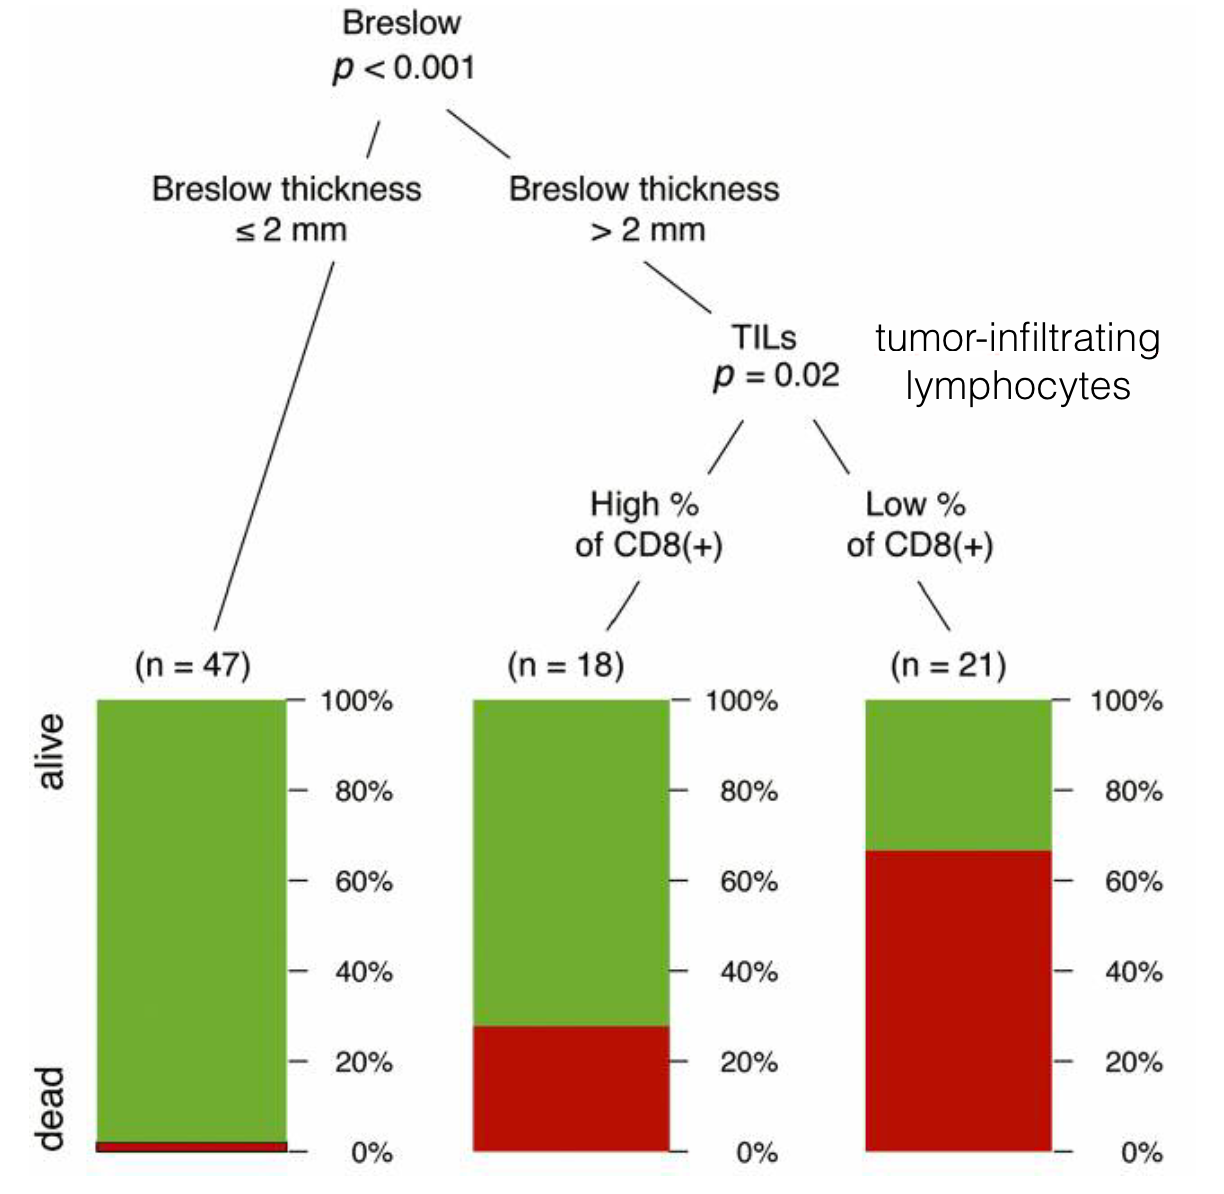
\includegraphics[width=0.5\linewidth]{figure/wbBILL8model} 

}

\caption{(fig:BILLCD8) Example tree model for melanoma risk}\label{fig:BILLCD8}
\end{figure}

Note, that being a white box model is not only about the structure, but
also about the number of parameters. A classification tree with 100s of
nodes is hard to understand, linear model with 100s of parameters is
hard to understand.

Things that are natural for white box models are hard for black box
models. For complex models we may not understand how and which features
influence the model decision, is the model consistent with the domain
knowledge. Tools presented in this book help to extract such information
even from complex models.

\hypertarget{model-agnostic-vs-model-specific}{%
\subsection{Model agnostic vs Model
specific}\label{model-agnostic-vs-model-specific}}

Some classes of models attract higher interest than others or are
developed for longer period of time. Thus some classes of models are
quipped with very good tools for model exploration or visualisation.
Just to mention some of them:

\begin{itemize}
\tightlist
\item
  Linear models have lots of tools for model diagnostic and validation
  of model assumptions. Assumptions are defined in a strict way
  (normality, linear structure, homogenous variance) and can be
  validated with normality tests or plots (qq plot), diagnostic plots,
  tests for model structure (RESET test), tools for identification of
  outliers etc.
\item
  More complex models with additive structure, like proportional hazards
  models have tools that verifies model assumptions.
\item
  Random Forest model is equipped with out of bag method of evaluation
  of performance and few tools for measuring variable importance
  \citep{R-randomForest}. Some tools were developed to extract
  information about possible interactions from the model structure
  \citep{R-randomForestExplainer}. Similar tools are developed to other
  ensembles of trees, like xgboost models \citep{R-xgboostExplainer}.
\item
  Neural Networks have large collection of dedicated explainers that use
  Layer-wise Relevance Propagation technique \citep{BachLWRP} or
  Saliency Maps technique \citep{SaliencyMaps} or a mixed approach.
\end{itemize}

List of model classes is much longer, and for every class there is a
collection of tools to use. But this variety of approaches leads to
problems. (1) One cannot easily compare explanations for two models with
different structures. (2) Every time when a new architecture of new
ensemble of models is proposed, we need to look for new methods of model
exploration. (3) For some new models we may not have yet any tool for
model explanation.

This book is focused on model agnostic techniques. Thus we do not assume
anything about model structure. The model will be threated as a black
box and the only operation that we will be able to perform is evaluation
of a model in a selected point.

Hoever, even if we do not assume anything about the model, we have some
assumptions about data. We assume that the model is a function of a form
\[
f: R^p \rightarrow R
\] i.e.~operates on a vector of \(p\) values. This assumption is most
suited with tabular data, is held for images, text data video and so on.
It may not be suited to models with states, or models with memory as
there the model output depends not only on model inputs.

Note also that if \(p\) is high dimensional then techniques described
here may not be enough to fully understand models with such large number
of degrees of freedom.

\hypertarget{why-do-we-need-model-explainers}{%
\subsection{Why do we need model
explainers?}\label{why-do-we-need-model-explainers}}

Machine Learning models have a wide range of applications in
classification or regression problems. Due to the increasing
computational power of computers and complexity of data sources, ML
models are becoming more and more sophisticated. Models created with the
use of techniques such as boosting or bagging of neural networks are
parametrized by thousands of coefficients. They are obscure; it is hard
to trace the link between input variables and model outcomes - in fact
they are treated as black boxes. They are used because of their
elasticity and high performance, but their deficiency in
interpretability is one of their weakest sides.

In many applications we need to know, understand or prove how the input
variables are used in the model. We need to know the impact of
particular variables on the final model predictions. Thus we need tools
that extract useful information from thousands of model parameters.

Tools for model exploration and model understanding have many
applications. They may be useful during every phase of a model
lifecycle.

Below we summaries how such tools will be useful during the model
development, model deployment or model maintenance.

\begin{figure}

{\centering 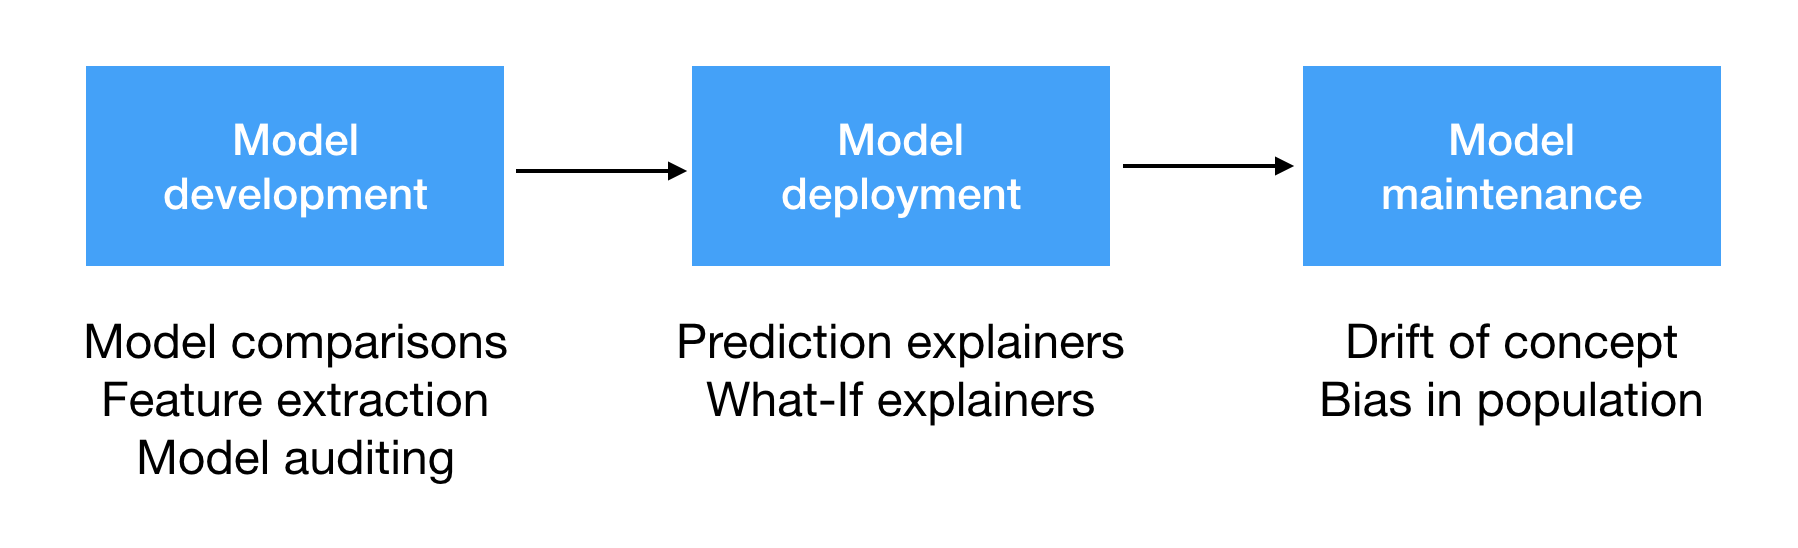
\includegraphics[width=0.9\linewidth]{figure/modelLifetime} 

}

\caption{(fig:modelLifetime) Example applications of explainers in different phases of model lifetime}\label{fig:modelLifetime}
\end{figure}

\textbf{Model development}

Model building or model development is a phase in which one is looking
for best available model.

In the Section \ref{partialDependence} we present tools for extraction
of relations between features and target variable. Such methods may be
used for feature engineering (assisted learning in which elastic black
box model is used to learn features for the white box model). Learning
from ML models may lead to model improvment.

In the Section \ref{modelComparisons} we present tools that helps to
compare models.

In the Section \ref{modelAuditing} we present tools that help to
validate model, audit model residuals, identify potential strange
behaviors.

If for some observations we observe lack of fit, then through tools
introduced in the Section \ref{variableAttributionMethods} we may verify
which variables do and which do not influence model decisions. This may
help to identify some problem in the model fit and in the end will help
to correct the model.

Since the AutoML methods are being more and more popular, model
explainers may actually help to understand how the model identified by
AutoML method is working.

If we identify cases on which model is not working properly, then model
explainers will help in model debugging. See an examples in the Section
TODO.

\textbf{Model deployment}

Model deployment is a phase in which one wants final use trust in model
decisions, understand these decisions and act accordingly. In some areas
complex models are not being adopted because people do not understand
nor trust them. Model explainers can change this and increase rate of
aquisition of new models

Since most people would not trust in recommendations, that they do not
understand, the key element here is to increase understanding related to
features that affect model decisions.

In the Section \ref{variableAttributionMethods} we introduce tools that
identify key features that drive model decisions.

In the Section \ref{ceterisParibus} we introduce tools for what-if
analysis of model decisions.

In some areas there may be leagal expectations or regulations that
requires that model predictions are explainable (see the right to
explanation). See \citep{2017arXiv171107076L} or
\citep{2017arXiv171006169T} for example methods that identify bias in
the data.

\textbf{Model maintenance}

Model maintenance is a phase in which one wants to make sure that model
is still valid and suited to the new data. Due to concept drift or
similar problems that may happen after some time, we need to monitor the
model performance.

In the section \ref{partialDependence} we present tools that may compare
how thw model response behaves on the new dataset. This helps to detect
flaws in model assumptions and biases in the data.

\hypertarget{how-model-exploration-is-different-from-data-exploration}{%
\subsection{How model exploration is different from data
exploration?}\label{how-model-exploration-is-different-from-data-exploration}}

Exploration and visualization of models is not that known as exploration
and visualization of data. As we will see in following chapters in both
cases we may use similar charts and similar way to express ideas. This
is because many people are already familiar with techniques for data
visualization and when we do model visualization we want to take
advantage of this knowledge.

Both in data visualization and in model visualization we use graphical
representation to deliver some messages quicker in a form that is easier
to digest. Despite all similarites we need to keep in mind few key
differences between these two wrods.

\begin{itemize}
\tightlist
\item
  Data is generated by some unknown phenomena and with data exploration
  and visualization we want to understand this phenomena. Models are
  created based on the data but in most cases we do not know how close
  are these models to unknown phenomena. So we do model exploration to
  validate if the model is correct. If the model is valid. In most cases
  we do not validate data if they are correct. So we are more skeptical
  about models than about data.
\item
  Data comes from some population; we treat data as a random sample, and
  there is some inherited randomness related to the sampling. On the
  opposite, models are just functions. Most models are not stochastic
  (or at least some models are not stochastic) and the randomness (if
  any) come from the fitting procedure not from the sampling.
\item
  Models may be inaccurate or biased. When we ask question like ,,How
  the model is working?'`we also ask ,,Is the model accurate, can I
  trust it, does it behave well, how much I can trust it?''. Similar
  question related to data do not question the data but question our
  understating of the data.
\end{itemize}

To summaries. We may use similar techniques. But they are used to answer
different questions.

\hypertarget{code-snippets}{%
\subsection{Code snippets}\label{code-snippets}}

TODO: Here we should tell why we present examples for DALEX. And mention
that there are also other functions that can be used.

\hypertarget{glossary-notation}{%
\subsection{Glossary / Notation}\label{glossary-notation}}

Let \(f_{M}(x): \mathcal R^{d} \rightarrow \mathcal R\) denote a
predictive model, i.e.~function that takes \(d\) dimensional vector and
calculate numerical score. Dimenstions of the vector \(x\) refer to
different variables (aka features).

In sections in which we work with larger number of models we use
subscript \(M\) to index models. But to simplify notation, this
subscript is omitted if profiles for only one model are considered.

Symbol \(x \in \mathcal R^d\) refers to a point in the feature space. We
use subscript \(x_i\) to refer to a different data points and
superscript \(x^j\) to refer to specific dimensions. Additionally, let
\(x^{-j}\) denote all coordinates except \(j\)-th and let \(x|^j=z\)
denote a data point \(x^*\) with all coordinates equal to \(x\) except
coordinate \(j\) equal to value \(z\). I.e.
\(\forall_{i \neq {j}} x^i = x^{*,i}\) and \(x^j = z\). In other words
\(x|^j=z\) denote a \(x\) with \(j\)th coordinate changed to \(z\).

\begin{itemize}
\tightlist
\item
  \emph{Black-box model} is a model with structure that is hard to
  understand for humans. Usually it refers to the number of model
  parameters. As different humans may be better in understanding more or
  less complex models, there is no strict threshold that makes model a
  black-box. But in practice for most humans this threshold is closed to
  10 rather than 100.
\item
  \emph{White-box model}, opposite to Black-box model, is a model that
  is easy to understand to human. Maybe not for every human. Consider
  small linear models and small CAR trees as white box models.
\item
  \emph{Feature} or \emph{Variable}, part of the model input space.
  Without large loss of generality we can assume that one feature is a
  single dimension in the input space. There are exceptions (among them:
  polynomials, interactions between variables, nominal variables), but
  they do not change the intuition.
\item
  \emph{Continuous variable}, a variable that can be presented as a
  number and the ordering makes some sense (zip codes or phone numbers
  are not considered as continuous variables). It does not need to be
  continuous in a mathematical sense. Counting variables (number of
  floors, steps) counts here as well.
\item
  \emph{Nominal variable}, opposite to \emph{Continuous variables},
  finite set of values that will not the threaded as a numeric
\end{itemize}

\hypertarget{thanksto}{%
\subsection{Acknowledgements}\label{thanksto}}

My work on interpretability has started during research trips within the
RENOIR project (691152 - H2020/2016-2019). So I would like to thank
prof. Janusz Holyst for the chance to take part in this project.

I would thank prof. Chris Drake for her hospitality. This book will
never been created without perfect conditions that I found at your house
in Woodland.

Also I would like to thank our editor John Kimmel. It is amazing, than
when only I mention his name to authors, I always hear that he is the
best editor they ever had.

This book is prepared with the \textbf{bookdown} package
\citep{R-bookdown}, thanks to amazing work of Yihui Xie.

\hypertarget{prediction-level-explanations}{%
\section*{Prediction level
explanations}\label{prediction-level-explanations}}
\addcontentsline{toc}{section}{Prediction level explanations}

\hypertarget{PredictionExplainers}{%
\section{Introduction}\label{PredictionExplainers}}

Prediction level explainers help to understand how the model works for a
single prediction. This is the main difference from the model level
explainers that were focused on the model as a whole and on model
population for whole population. Prediction level explainers work in the
context of single observations.

Think about following use-cases

\begin{itemize}
\tightlist
\item
  One wants to attribute effects of variables to a model predictions.
  Think about model for heart accident Having a final score for a
  particular patient one wants to understand how much of this score can
  be attributed to smoking or age or gender.
\item
  One wants to understand how the model response would change if some
  inputs are changed. Again, think about model for heart accident How
  the model response would change if a patient cuts the number of
  cigarettes per day by half. Or if he introduces a low-carbon diet.
\item
  Model is not working correctly for a particular point and one wants to
  understand why predictions for this point are wrong. Think about
  patient that had heart accident but his risk score is very low. One
  wants to understand which factors may be overlooked.
\end{itemize}

\hypertarget{approaches-to-prediction-explanations}{%
\subsection{Approaches to prediction
explanations}\label{approaches-to-prediction-explanations}}

There are many different tools that may be used to explore model around
a single point \(x^*\). Model is a function that takes \(p\) dimensional
vector as an input. Thus to plot this function we would need \(p+1\)
dimensions.

An toy example with \(p=2\) is presented in Figure
\ref{fig:cutsSurfaceReady}. We will use it as an illustration of key
ideas.

\begin{figure}

{\centering 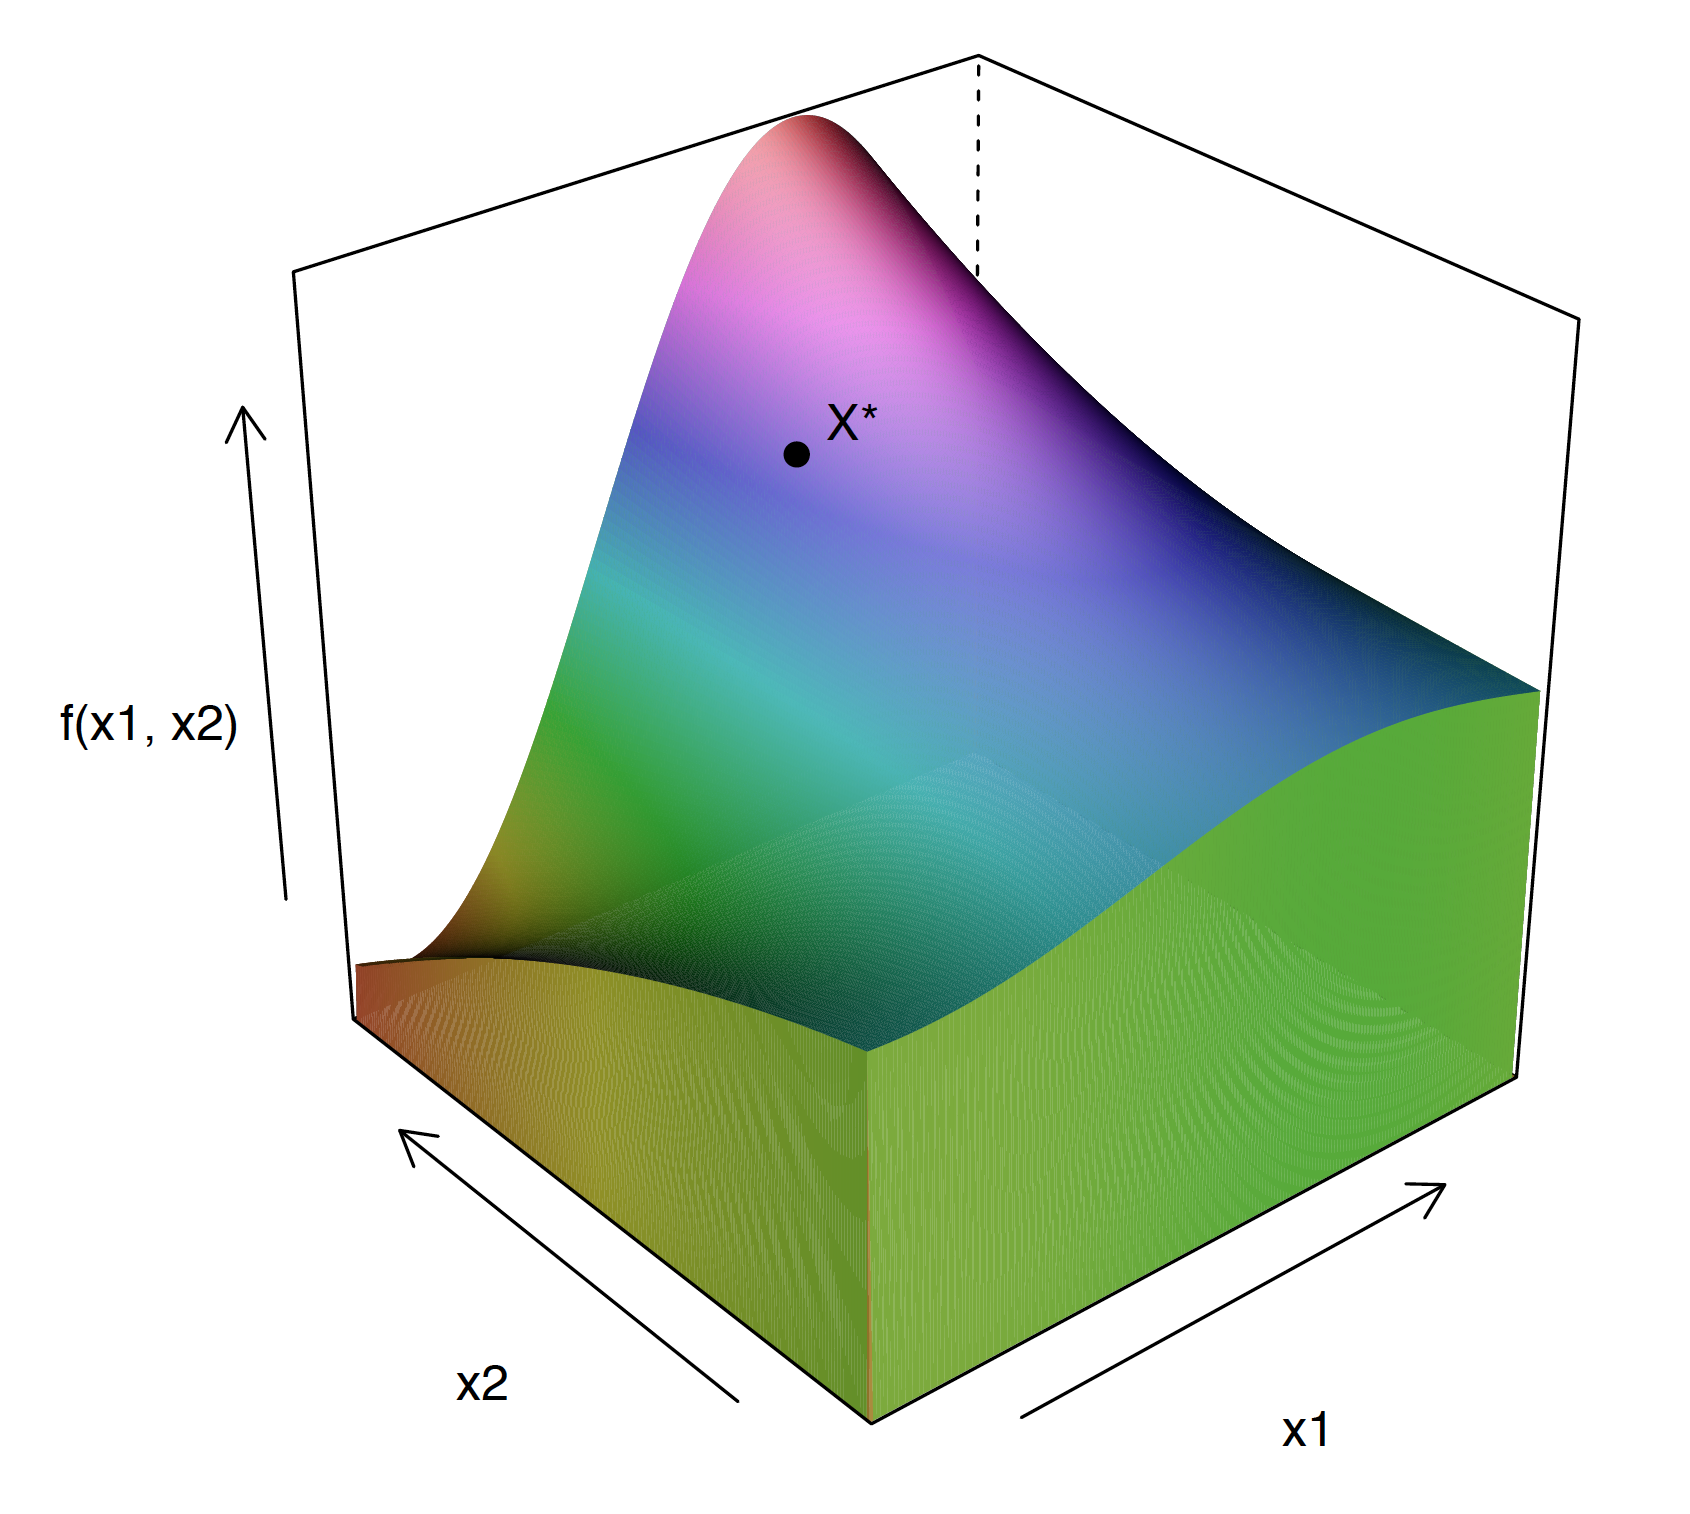
\includegraphics[width=0.6\linewidth]{figure/cuts_surface_ready_punkt} 

}

\caption{(fig:cutsSurfaceReady) Model response surface. Here the model is a function of two variables.  We are interested in understanding the response of a model in a single point x*}\label{fig:cutsSurfaceReady}
\end{figure}

In following sections we will describe the most popular approaches to
exploration of such function. They can be divided into three classes.

\begin{itemize}
\tightlist
\item
  One approach to exploration of model response is to investigate how
  the model response would change if single variable in the model input
  would change. This way we may observe profiles seen as a function of a
  single variable. Such profiles are usually called Ceteris Paribus
  Profiles. We will present them in detail in the Section
  \ref{ceterisParibus}. This is useful for What-If scenarios. See an
  example in Figure \ref{fig:cutsTechnikiReady} panel A.
\item
  Other approach is to analyze model curvature around point of interest.
  Again we treat the model as a function and we are interested in the
  local behavior of this function around the point of interest. We
  approximate the black-box model with a simpler white-box model around
  point \(x^*\). See an example in Figure \ref{fig:cutsTechnikiReady}
  panel B. In the Section \ref{LIME} we present the LIME method that
  exploits the concept of local model.
\item
  Yet another approach is to analyze how the model response in point
  \(x^*\) is different from the average model response. And how the
  difference can be distributed between model behavior along different
  dimensions. See an example in Figure \ref{fig:cutsTechnikiReady} panel
  C. In the Section \ref{variableAttributionMethods} we present two
  methods for variable contributions, sequential conditioning and
  average conditioning (called also Shapley values).
\end{itemize}

\begin{figure}

{\centering 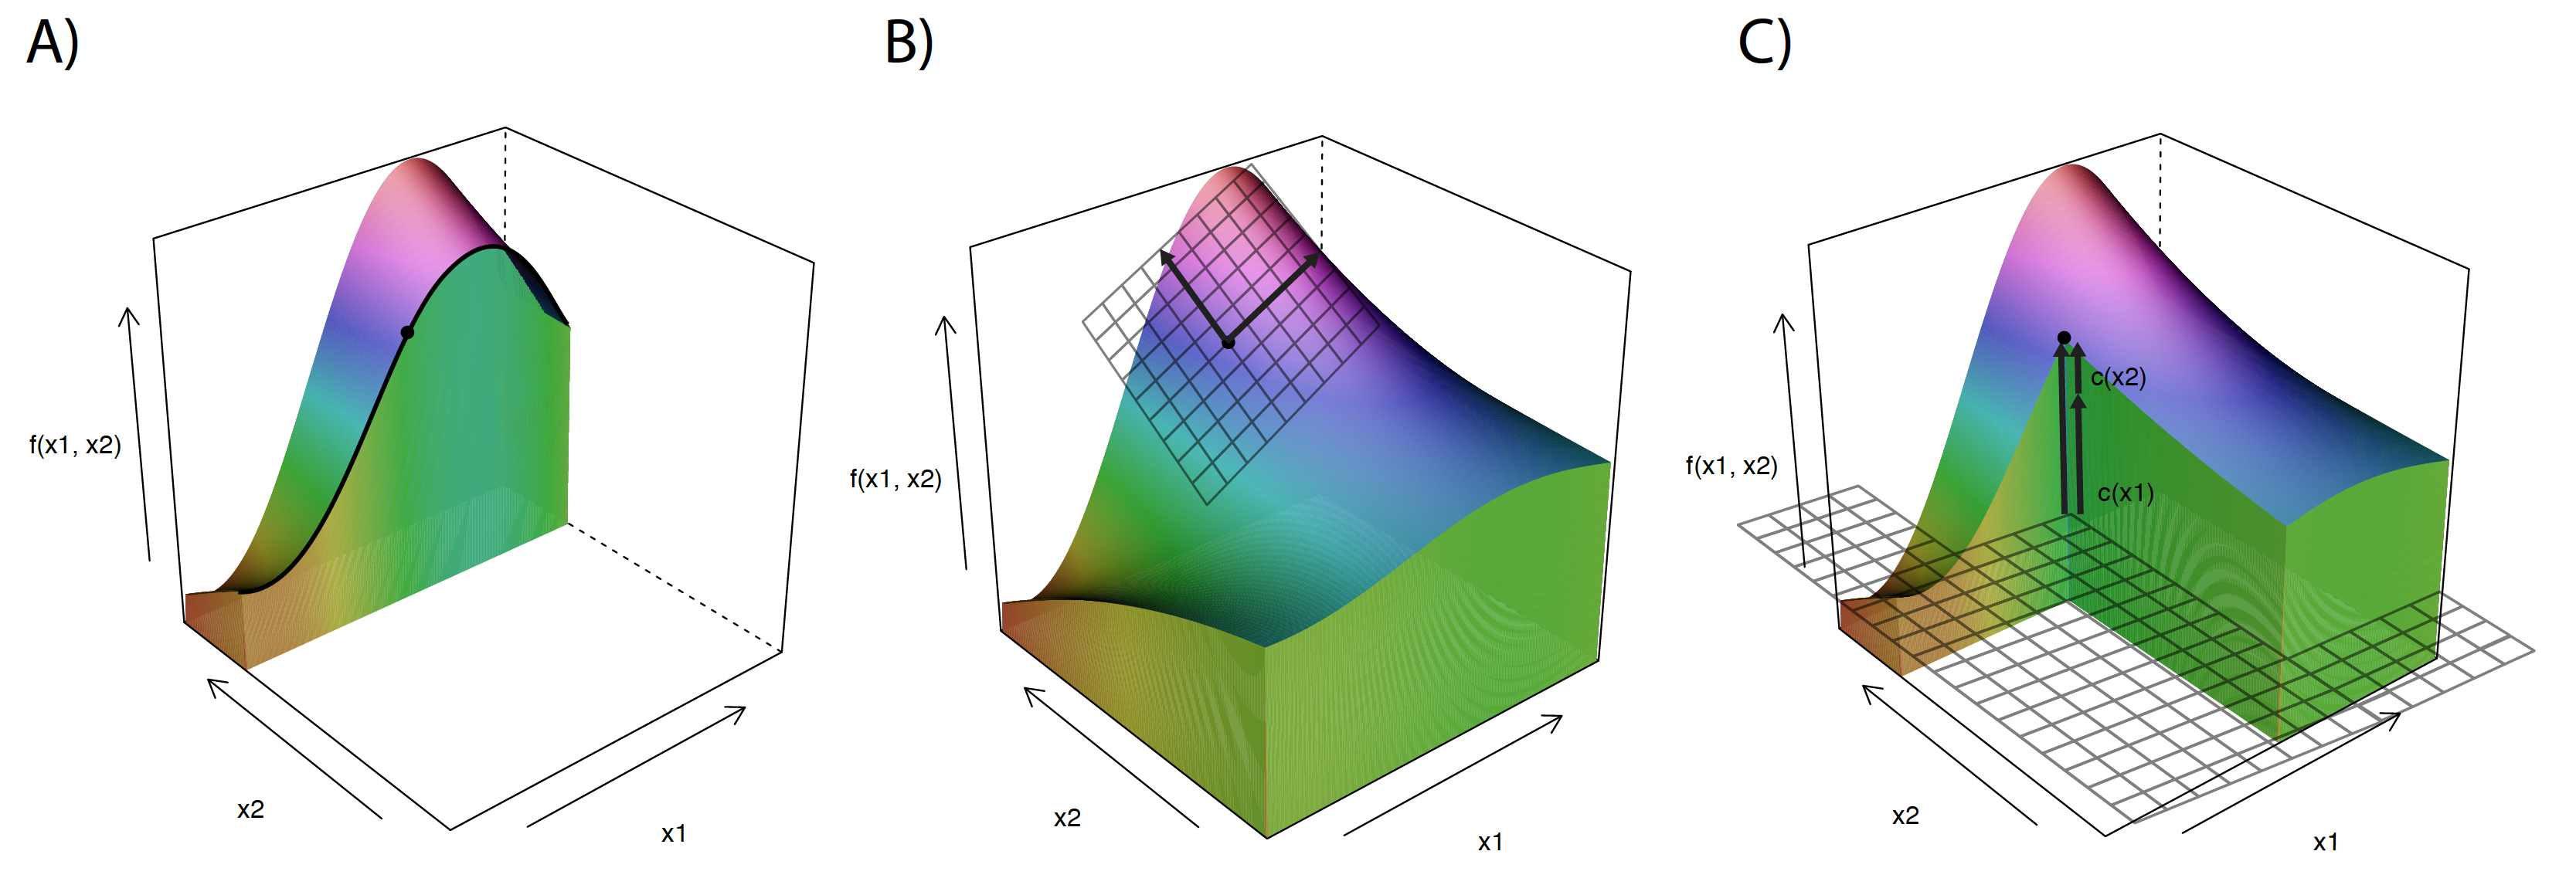
\includegraphics[width=0.99\linewidth]{figure/cuts_techniki_ready} 

}

\caption{(fig:cutsTechnikiReady) Intuitions behind different approached to prediction level explainers. Panel A presents an idea behind What-If analysis with Ceteris Paribus profiles. Keeping all other variables unchanged we trace model response along changes in a single variable. Panel B presents an idea behind local models like LIME. A simpler white-box model is fitted around the point of interest. It describes the local behaviour of the complex model. Panel C presents an idea behind variable attributions. Additive effects of each variable show how the model response differs from population average.}\label{fig:cutsTechnikiReady}
\end{figure}

\hypertarget{three-single-laws}{%
\subsection{A bit of philosophy: Three Laws for Prediction Level
Explanations}\label{three-single-laws}}

76 years ago Isaac Asimov devised
\href{https://en.wikipedia.org/wiki/Three_Laws_of_Robotics}{Three Laws
of Robotics}: 1) a robot may not injure a human being, 2) a robot must
obey the orders given it by human beings and 3) A robot must protect its
own existence. These laws impact discussion around
\href{https://en.wikipedia.org/wiki/Ethics_of_artificial_intelligence}{Ethics
of AI}. Today's robots, like cleaning robots, robotic pets or autonomous
cars are far from being conscious enough to be under Asimov's ethics.

Today we are surrounded by complex predictive algorithms used for
decision making. Machine learning models are used in health care,
politics, education, judiciary and many other areas. Black box
predictive models have far larger influence on our lives than physical
robots. Yet, applications of such models are left unregulated despite
many examples of their potential harmfulness. See \emph{Weapons of Math
Destruction} by Cathy O'Neil \citep{ONeil} for an excellent overview of
selected problems.

It's clear that we need to control algorithms that may affect us. Such
control is in our civic rights. Here we propose three requirements that
any predictive model should fulfill.

\begin{itemize}
\tightlist
\item
  \textbf{Prediction's justifications}. For every prediction of a model
  one should be able to understand which variables affect the prediction
  and how strongly. Variable attribution to final prediction.
\item
  \textbf{Prediction's speculations}. For every prediction of a model
  one should be able to understand how the model prediction would change
  if input variables were changed. Hypothesizing about what-if
  scenarios.
\item
  \textbf{Prediction's validations} For every prediction of a model one
  should be able to verify how strong are evidences that confirm this
  particular prediction.
\end{itemize}

There are two ways to comply with these requirements. One is to use only
models that fulfill these conditions by design. White-box models like
linear regression or decision trees. In many cases the price for
transparency is lower performance. The other way is to use approximated
explainers -- techniques that find only approximated answers, but work
for any black box model. Here we present such techniques.

\hypertarget{variableAttributionMethods}{%
\section{Variable attribution for linear
models}\label{variableAttributionMethods}}

In this section we introduce the concept and the intuition behind
additive decompositions of model predictions. The main goal for these
tools is to help to understand how model output may be decomposed into
parts, that can be attributed to input features.

Presented explainers are linked with the first law introduced in Section
\ref{three-single-laws}, i.e.~law for prediction's justifications. Note
that there is a collection of tools for variable attribution. In this
section we are focused on the general idea and examples for linear
models. Model agnostic approaches will be presented in sections
\ref{breakDown} and \ref{shapley}.

Think of following use cases:

\begin{itemize}
\tightlist
\item
  Think about a model for heart attack. A patient wants to know which
  factors have highest impact on the final heart risk score.
\item
  Think about a model for apartment prices. An investor wants to know
  how much of the final price may be attributed to the location of an
  apartment.
\item
  Think about a model for credit scoring. A customer wants to know if
  factors like gender, age or number of kids influence model decisions.
\end{itemize}

In every usecase one needs to attribute part of the model response to a
single variable. This can be done directly for linear models, so in the
section \ref{VAlinMod} we show how to do this for linar models and may
be easily extended to additive models and generalized linear models. For
other models it is not trivial how to do so, some approaches are be
presented in next sections.

\hypertarget{intuition}{%
\subsection{Intuition}\label{intuition}}

Fiited linear model with coefficients
\(\beta = (\beta_0, \beta_1, .., \beta_p)\) has following form.

\[
f(x) = \beta_0 + x_1 \beta_1 + \ldots + x_p \beta_p.
\] In other words, model response is the sum of weighted elements of
\(x = (x_1, x_2, \ldots, x_p)\).

From a global perspective of a model, we are usually interested in
questions like, how good is the model (questions about \(R^2\)), which
variables are significant (tests for significance of \(\beta_i \neq 0\))
or how accurate are model predictions (confidence intervals for
predictions).

But in this chapter we are focued on a local perspective, i.e.~for a
single observation \(x^*\) how to measure the contribution of a variable
\(x_i\) on model prediction \(f(x^*)\).

The contribution of a variable \(x_i\) shall be related to
\(x^*_i\beta_i\) as variable \(x_i\) occur only in this term. As we will
see below, it is easier to interpret variable contribution if the
\(x_i\) is centered.

This lead for a intuitive formula for variable attribution for model
\(f\), variable \(x_i\) in the point \(x^*\) \[
v(f, x^*, i) = \beta_i (x_i^* - \hat x_i).
\]

\hypertarget{method}{%
\subsection{Method}\label{method}}

We want to calculate \(v(f, x^*, i)\), which is the contribution of
variable \(x_i\) on prediction of model \(f()\) in point \(x^*\).

Geneal approach for calculation of variable attributions would be to
measure how much the expected model response would change after
conditioning on \(x_i = x_i^*\).

\[
v(f, x^*, i) = E[f(x) | x_i = x_i^*] - E[f(x)]
\]

For linear models, if coordinates of \(x\) are independent, this is
equivalent of

\[
v(f, x^*, i) = f(x^*) - E[f(x)|x_{-i} = x^*_{-i}] = \beta_i x^*_i  - E \beta_i X_i.
\] Expected value can be estimated as averages, and this leads to\\
\[
v(f, x^*, i) = \beta_i x^*_i - \beta_i \bar x_i = \beta_i (x^*_i - \bar x_i)
\]

The logic behind the attribution is the following. Contribution of
variable \(x_i\) is the difference between model response for value
\(x_i^*\) minus the average model response.

Note that the linear model ma be rewritten in a following way

\[
f(x) = baseline + (x_1 - \bar x_1) \beta_1 + ... + (x_p - \bar x_p) \beta_p
\]

where \[
baseline = \mu + \bar x_1 \beta_1 + ... + \bar x_p \beta_p.
\]

Here \(baseline\) is an average model response and variable
contributions show how prediction for particular \(x^*\) is different
from the average response.

** NOTE for careful readers **

There is a gap between expected value of \(X_i\) and average calculated
on some dataset \(\bar x_i\). The latter depends on the data used for
calculation of averages. For the sake of simplicity we do not emphasize
these differences. To live with this just assume that we have access to
a very large validation data that allows us to calculate \(\bar x_i\)
very accurately.

Also we assumed that coordinated of \(x\) are independent, which may not
be the case. We will return to this problem later, during the discussion
related to interactions.

\hypertarget{example-wine-quality}{%
\subsection{Example: Wine quality}\label{example-wine-quality}}

It may be a surprise, that the attribution for variable \(x_i\) is not
the \(\beta_i x_i\). To understand this, consider following example.

\begin{figure}

{\centering 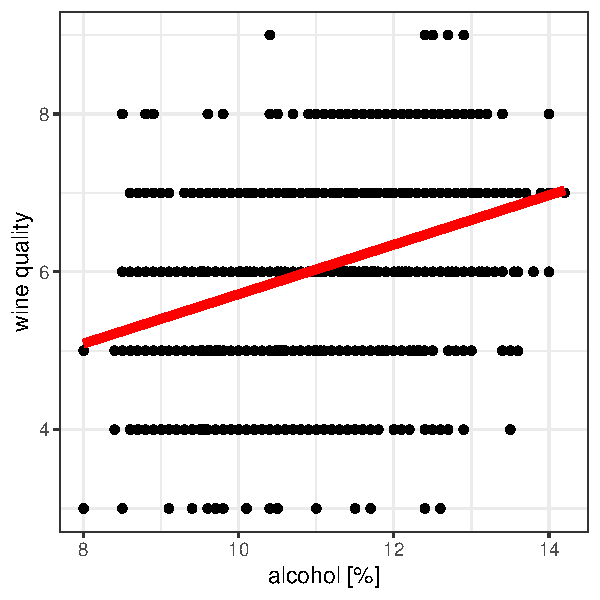
\includegraphics[width=0.5\linewidth]{figure/attribution_1} 

}

\caption{(fig:attribution1)Relation between wine quality and concentration of alcohol assessed with linear model}\label{fig:attribution1}
\end{figure}

Figure \ref{fig:attribution1} shows the relation between alcohol and
wine quality, based on the wine dataset \citep{wine2009}. The
corresponding linear model is

\[
quality(alcohol) = 2.5820 + 0.3135 * alcohol
\]

The weakest wine in this dataset has 8\% of alcohol, average alcohol
concentration is 10.51, so the contribution of alcohol to the model
prediction is \(0.3135 *(8-10.51) = -0.786885\). It means that low value
of alcohol for this wine (8\%) lower the prediction of quality by
\(-0.786885\).

Note, that it would be confusing to use \(x_i\beta_i\) as alcohol
contribution on quality would be \(0.3135*8 = 2.508\). This would not
reflect the intuition that for positive relation, the smaller is the
alcohol concentration the lower should be the quality of wine.

\hypertarget{pros-and-cons}{%
\subsection{Pros and Cons}\label{pros-and-cons}}

Here we summarise pros and cons of this approach.

\textbf{Pros}

\begin{itemize}
\tightlist
\item
  Presented variable attribution for linear model is not an
  approximation, it is directly linked with the structure of a model.
\item
  It is easier to understand attributions that are not linked with scale
  nor location of \(x_i\) as the standard \(\beta_i\) are.
\end{itemize}

\textbf{Cons}

\begin{itemize}
\tightlist
\item
  It works only for linear models.
\item
  This do not reduce model complexity. Just present model coefficients
  in a different way.
\end{itemize}

\hypertarget{code-snippets-1}{%
\subsection{Code snippets}\label{code-snippets-1}}

Variable attributions for linear models may be directly extracted from
the \texttt{predict()} function for linear models.

In this section we will present an example for logistic regression based
on the \texttt{HR} dataset. See the Section \ref{HRdataset} for more
details.

First we build a logistic regression model for binary variable
\texttt{status\ ==\ "fired"}. Here are fitted model coefficients.

\begin{Shaded}
\begin{Highlighting}[]
\KeywordTok{library}\NormalTok{(}\StringTok{"DALEX"}\NormalTok{)}
\NormalTok{model_fired <-}\StringTok{ }\KeywordTok{glm}\NormalTok{(status }\OperatorTok{==}\StringTok{ "fired"} \OperatorTok{~}\StringTok{ }\NormalTok{., }\DataTypeTok{data =}\NormalTok{ HR, }\DataTypeTok{family =} \StringTok{"binomial"}\NormalTok{)}
\KeywordTok{coef}\NormalTok{(model_fired)}
\end{Highlighting}
\end{Shaded}

\begin{verbatim}
##  (Intercept)   gendermale          age        hours   evaluation 
##  5.737945729 -0.066803609 -0.001503314 -0.102021120 -0.425793369 
##       salary 
## -0.015740080
\end{verbatim}

We want to calculate variable attributions for a particular point. Here
we define this point.

\begin{Shaded}
\begin{Highlighting}[]
\NormalTok{new_observation <-}\StringTok{ }\KeywordTok{data.frame}\NormalTok{(}\DataTypeTok{gender =} \KeywordTok{factor}\NormalTok{(}\StringTok{"male"}\NormalTok{, }\DataTypeTok{levels =} \KeywordTok{c}\NormalTok{(}\StringTok{"male"}\NormalTok{, }\StringTok{"female"}\NormalTok{)),}
                      \DataTypeTok{age =} \FloatTok{57.7}\NormalTok{,}
                      \DataTypeTok{hours =} \FloatTok{42.3}\NormalTok{,}
                      \DataTypeTok{evaluation =} \DecValTok{2}\NormalTok{,}
                      \DataTypeTok{salary =} \DecValTok{2}\NormalTok{)}
\end{Highlighting}
\end{Shaded}

For linear and generalized linear models we may specify argument
\texttt{type\ =\ "terms"} that extracts variable contributions.

\begin{Shaded}
\begin{Highlighting}[]
\KeywordTok{predict}\NormalTok{(model_fired, new_observation, }\DataTypeTok{type =} \StringTok{"terms"}\NormalTok{)}
\end{Highlighting}
\end{Shaded}

\begin{verbatim}
##        gender         age     hours evaluation      salary
## 1 -0.03361889 -0.02660691 0.7555555  0.5547197 0.007287334
## attr(,"constant")
## [1] -0.8714962
\end{verbatim}

Below we show how to do this with the \texttt{DALEX} package.
Additionaly we may easily plot contributions.

\begin{Shaded}
\begin{Highlighting}[]
\KeywordTok{library}\NormalTok{(}\StringTok{"DALEX"}\NormalTok{)}

\NormalTok{explainer_fired <-}\StringTok{ }\KeywordTok{explain}\NormalTok{(model_fired,}
                 \DataTypeTok{data =}\NormalTok{ HR,}
                 \DataTypeTok{y =}\NormalTok{ HR}\OperatorTok{$}\NormalTok{status }\OperatorTok{==}\StringTok{ "fired"}\NormalTok{,}
                 \DataTypeTok{label =} \StringTok{"fired"}\NormalTok{)}

\NormalTok{attribution <-}\StringTok{ }\KeywordTok{single_prediction}\NormalTok{(explainer_fired, new_observation)}
\NormalTok{attribution}
\end{Highlighting}
\end{Shaded}

\begin{verbatim}
##                   variable contribution variable_name variable_value
## 1              (Intercept)  0.000000000     Intercept              1
## hours         hours = 42.3  0.755555494         hours           42.3
## evaluation  evaluation = 2  0.554719716    evaluation              2
## gender       gender = male -0.033618893        gender           male
## age             age = 57.7 -0.026606908           age           57.7
## salary          salary = 2  0.007287334        salary              2
## 11         final_prognosis  1.257336743                             
##            cummulative sign position label
## 1            0.0000000    0        1 fired
## hours        0.7555555    1        2 fired
## evaluation   1.3102752    1        3 fired
## gender       1.2766563   -1        4 fired
## age          1.2500494   -1        5 fired
## salary       1.2573367    1        6 fired
## 11           1.2573367    X        7 fired
\end{verbatim}

\begin{Shaded}
\begin{Highlighting}[]
\KeywordTok{plot}\NormalTok{(attribution)}
\end{Highlighting}
\end{Shaded}

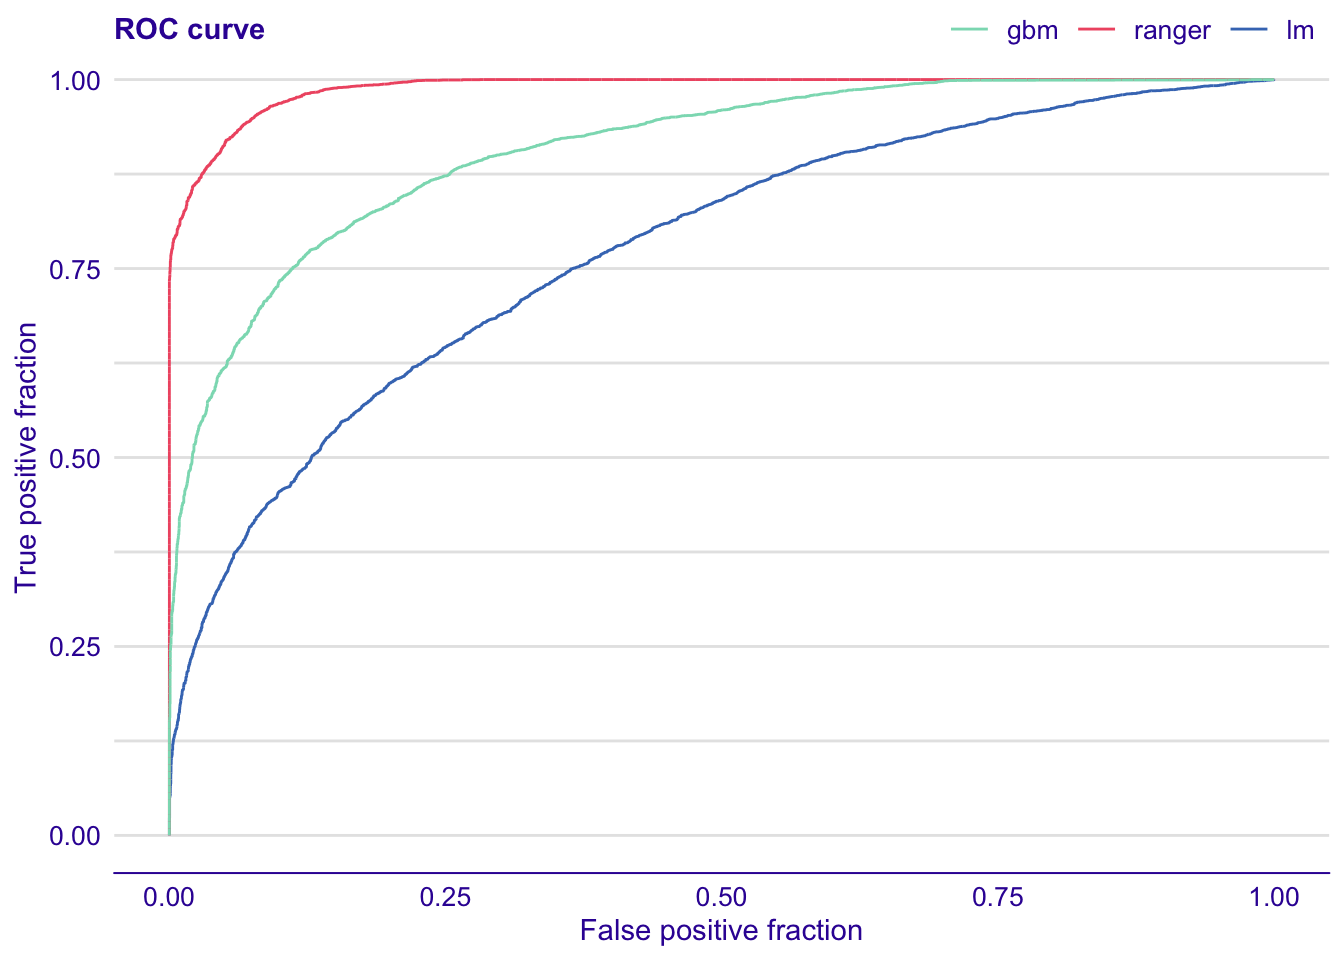
\includegraphics{PM_VEE_files/figure-latex/unnamed-chunk-4-1.pdf}

\hypertarget{breakDown}{%
\section{Sequential variable attributions}\label{breakDown}}

In the Section \ref{variableAttributionMethods} we introduced a method
for calculation of variable attributions for linear models. This method
is accurate, based directly on the structure of the model. But for most
popular machine learning models we cannot assume that they are linear
nor even additive.

\hypertarget{intuition-1}{%
\subsection{Intuition}\label{intuition-1}}

For any model we may repeat the intuition presented in Section
\ref{variableAttributionMethods} to calculate variable contribution as
shifts in expected model response after conditioning over consecutive
variables. This intuition is presented in Figure \ref{BDPrice4}.

Panel A shows distribution of model responses. The row
\texttt{all\ data} shows the model response of the original dataset. The
red dot stands for average is is an estimate of expencted model response
\(E [f(x)]\).

Since we want to calculate effects of particular values of selected
variables we then condition over these variables in a sequential manner.
The next row in panel A corresponds to average model prediction for
observations with variable \texttt{surface} fixed to value \texttt{35}.
The next for corresponds to average model prediction with variables
\texttt{surface} set to \texttt{35} and \texttt{floor} set to
\texttt{1}, and so on. The top row corresponds to model response for
\(x^*\).

Black lines in the panel A show how prediction for a single point
changes after coordinate \(i\) is repaced by the \(x^*_i\). But finaly
we are not interestes in particular changes, not even in distributions
but only in averages - expected model responses.

The most minimal form that shows important information is presented in
the panel C. Positive values are presented with green bars while
negative differences are marked with yellow bar. They sum up to final
model prediction, which is denoted by a grey bar in this example.

\begin{figure}

{\centering 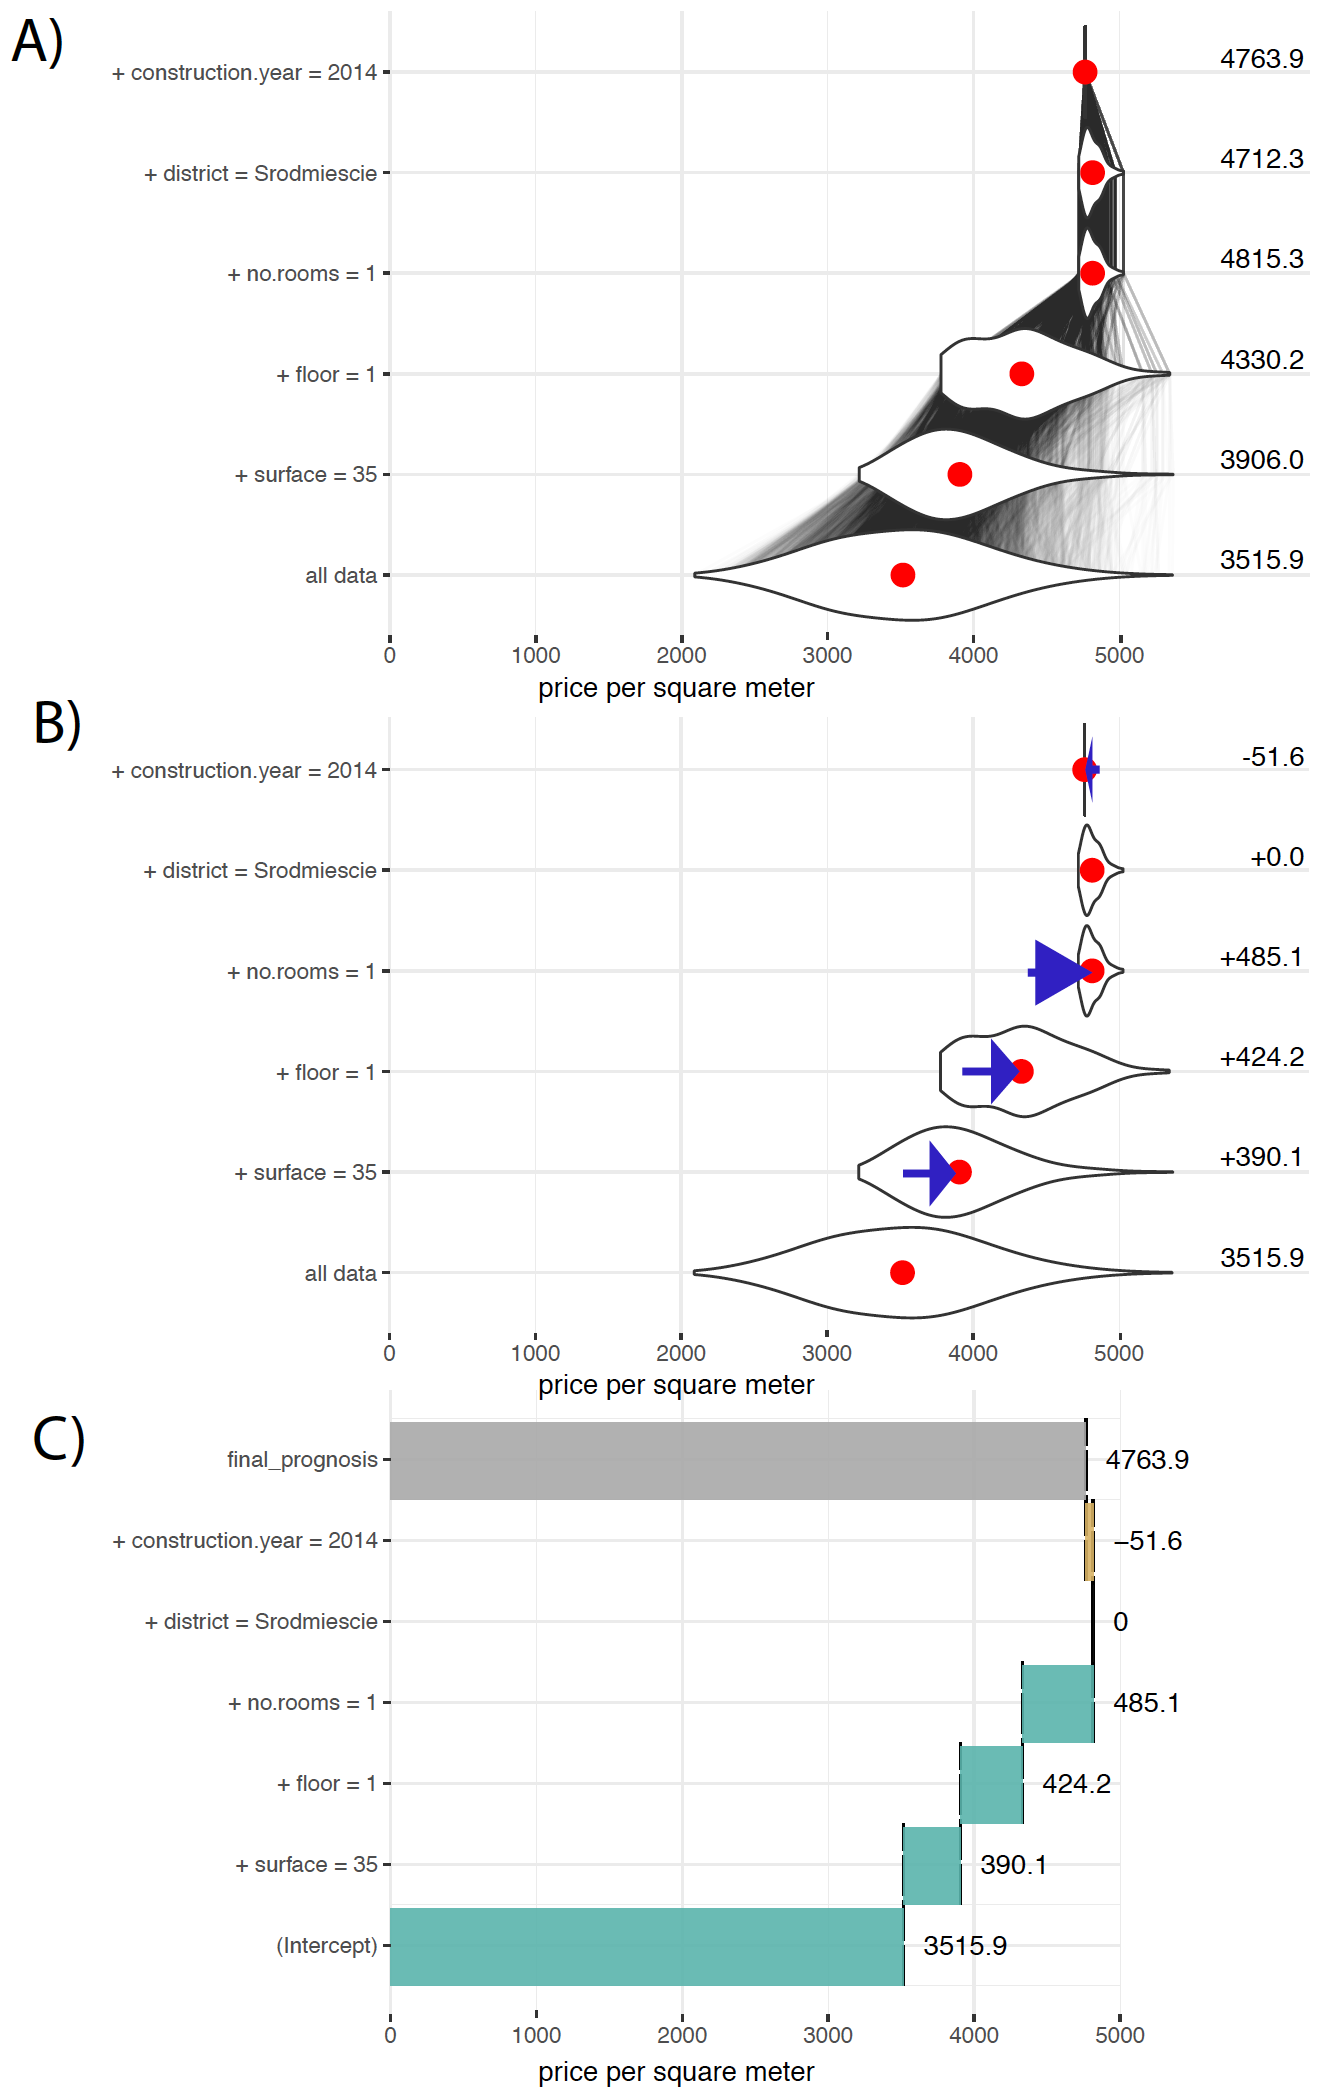
\includegraphics[width=0.7\linewidth]{figure/bd_price_4} 

}

\caption{(fig:BDPrice4) Break Down Plots show how variables move the model prediction from population average to the model prognosis for a single observation. A) The last row shows distribution of model predictions. Next rows show conditional distributions, every row a new variable is added to conditioning. The first row shows model prediction for a single point. Red dots stand for averages. B) Blue arrows shows how the average conditional response change, these values are variables contributions. C) Only variable contributions are presented. }\label{fig:BDPrice4}
\end{figure}

\hypertarget{method-1}{%
\subsection{Method}\label{method-1}}

Again, let \(v(f, x^*, i)\) stands for the contribution of variable
\(x_i\) on prediction of model \(f()\) in point \(x^*\).

We expect that such contribution will sum up to the model prediction in
a given point (property called \emph{local accuracy}), so \[
f(x^*) = baseline + \sum_{i=1}^p v(f, x^*, i)
\] where \(baseline\) stands for average model response.

Note that the equation above may be rewritten as

\[
E [f(X)|X_1 = x_1^*, \ldots, X+p = x_p^*] = E[f(X)] + \sum_{i=1}^p v(f, x^*, i)
\] what leads to quite natural proposition for \(v(f, x^*_i, i)\), such
as

\[
v(f, x^*_i, i) = E [f(X) | X_1 = x_1^*, \ldots, X_i = x_i^*] - E [f(X) | X_1 = x_1^*, \ldots, X_{i-1} = x_{i-1}^*] 
\] In other words the contribution of variable \(i\) is the difference
between expected model response conditioned on first \(i\) variables
minus the model response conditioned on first \(i-1\) variables.

Such proposition fulfills the \emph{local accuracy} condition, but
unfortunatelly variable contributions depends on the ordering of
variables.

\begin{figure}

{\centering 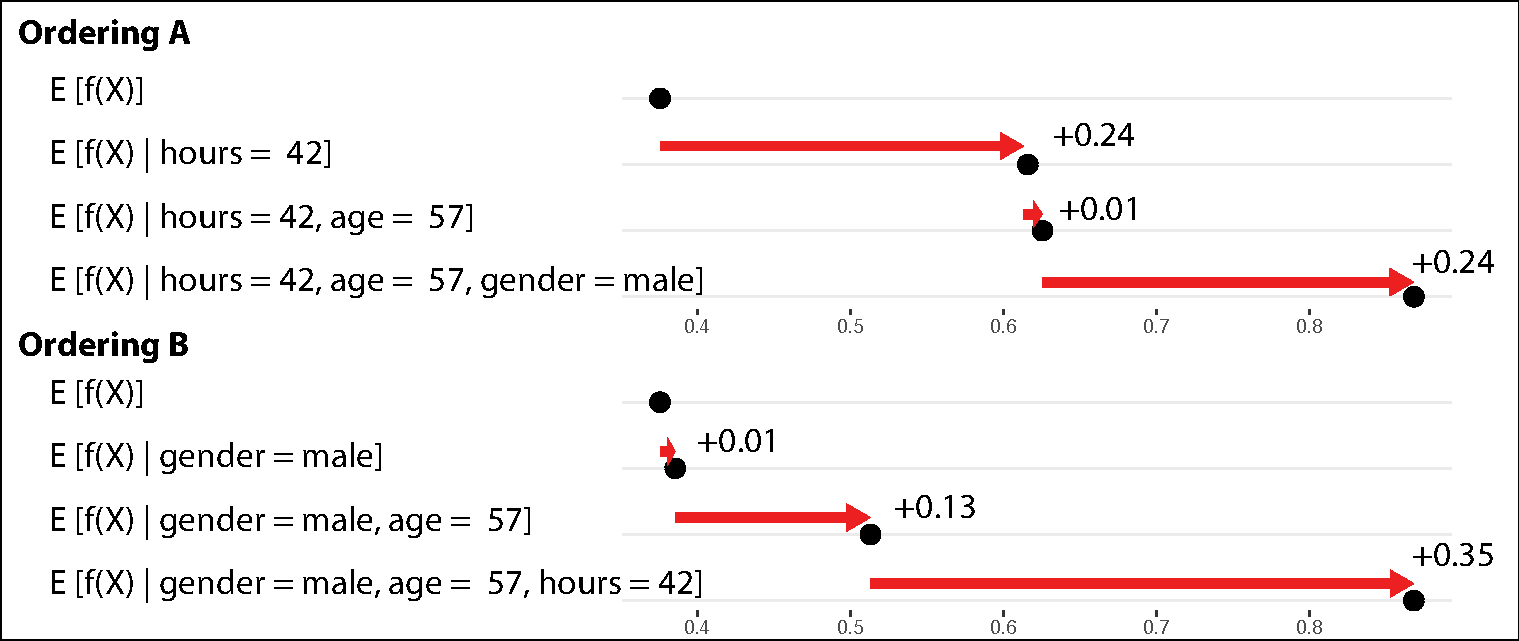
\includegraphics[width=1\linewidth]{figure/ordering} 

}

\caption{(fig:ordering) Two different paths between average model prediction and the model prediction for a selected observation. Black dots stand for conditional average, red arrows stands for changes between conditional averages.}\label{fig:ordering}
\end{figure}

See for example Figure \ref{fig:ordering}. In the first ordering the
contribution of variable \texttt{age} is calculated as 0.01, while in
the second the contribution is calculated as 0.13. Such differences are
related to the lack of additivness of the model \(f()\). Propositions
presented in next two sections present different solutions for this
problem.

The approach for variable attribution presented in the Section
\ref{modelAgnosticAttribution} has the property of \emph{local
accuracy}, but variable contributions depends on the variable ordering.

The easiest way to solve this problem is to use two-step procedure. In
the first step variables are ordered and in the second step the
consecutive conditioning is applied to ordered variables.

First step of this algorithm is to determine the order of variables for
conditioning. It seems to be reasonable to include first variables that
are likely to be most important, leaving the noise variables at the end.
This leads to order based on following scores

\[
score(f, x^*, i) = \left| E [f(X)] - E [f(X)|X_i = x^*_i] \right|
\] Note, that the absolute value is needed as variable contributions can
be both positive and negative.

Once the ordering is determined in the second step variable
contributions are calculated as

\[
v(f, x^*_i, i) = E [f(X) | X_{I \cup \{i\}} = x_{I \cup \{i\}}^*] - E [f(X) | X_{I} = x_{I}^*] 
\] where \(I\) is the set of variables that have scores smaller than
score for variable \(i\).

\[
I = \{j: score(f, x^*, j) < score(f, x^*, i)\}
\]

The time complexity of the first step id \(O(p)\) where \(p\) is the
number of variables and the time complexity of the second step is also
\(O(p)\).

\hypertarget{example-hire-or-fire}{%
\subsection{Example: Hire or Fire?}\label{example-hire-or-fire}}

Let us consider a random forest model created for HR data. The average
model response is \(\bar f(x) = 0.385586\). For a selected observation
\(x^*\) the table below presents scores for particular variables.

\begin{longtable}[]{@{}lrr@{}}
\toprule
& Ei f(X) & scorei\tabularnewline
\midrule
\endhead
hours & 0.616200 & 0.230614\tabularnewline
salary & 0.225528 & 0.160058\tabularnewline
evaluation & 0.430994 & 0.045408\tabularnewline
age & 0.364258 & 0.021328\tabularnewline
gender & 0.391060 & 0.005474\tabularnewline
\bottomrule
\end{longtable}

Once we determine the order we can calculate sequential contributions

\begin{longtable}[]{@{}lrr@{}}
\toprule
variable & cumulative & contribution\tabularnewline
\midrule
\endhead
(Intercept) & 0.385586 & 0.385586\tabularnewline
* hours = 42 & 0.616200 & 0.230614\tabularnewline
* salary = 2 & 0.400206 & -0.215994\tabularnewline
* evaluation = 2 & 0.405776 & 0.005570\tabularnewline
* age = 58 & 0.497314 & 0.091538\tabularnewline
* gender = male & 0.778000 & 0.280686\tabularnewline
final\_prognosis & 0.778000 & 0.778000\tabularnewline
\bottomrule
\end{longtable}

\hypertarget{pros-and-cons-1}{%
\subsection{Pros and cons}\label{pros-and-cons-1}}

Break Down approach is model agnostic, can be applied to any predictive
model that returns a single number. It leads to additive variable
attribution. Below we summarize key strengths and weaknesses of this
approach.

\textbf{Pros}

\begin{itemize}
\tightlist
\item
  Break Down Plots are easy to understand and decipher.
\item
  Break Down Plots are compact; many variables may be presented in a
  small space.
\item
  Break Down Plots are model agnostic yet they reduce to intuitive
  interpretation for linear Gaussian and generalized models.
\item
  Complexity of Break Down Algorithm is linear in respect to the number
  of variables.
\end{itemize}

\textbf{Cons}

\begin{itemize}
\tightlist
\item
  If the model is non-additive then showing only additive contributions
  may be misleading.
\item
  Selection of the ordering based on scores is subjective. Different
  orderings may lead to different contributions.
\item
  For large number of variables the Break Down Plot may be messy with
  many variables having small contributions.
\end{itemize}

\hypertarget{code-snippets-for-r}{%
\subsection{Code snippets for R}\label{code-snippets-for-r}}

In this section we present key features of the \texttt{breakDown}
package for R \citep{R-breakDown}. This package covers all features
presented in this chapter. It is available on CRAN and GitHub. Find more
examples at the website of this package
\texttt{https://pbiecek.github.io/breakDown/}.

\textbf{Model preparation}

In this section we will present an example based on the \texttt{HR}
dataset and Random Forest model \citep{R-randomForest}. See the Section
\ref{HRdataset} for more details.

\begin{Shaded}
\begin{Highlighting}[]
\KeywordTok{library}\NormalTok{(}\StringTok{"DALEX"}\NormalTok{)}
\KeywordTok{library}\NormalTok{(}\StringTok{"randomForest"}\NormalTok{)}
\NormalTok{model <-}\StringTok{ }\KeywordTok{randomForest}\NormalTok{(status }\OperatorTok{~}\StringTok{ }\NormalTok{gender }\OperatorTok{+}\StringTok{ }\NormalTok{age }\OperatorTok{+}\StringTok{ }\NormalTok{hours }\OperatorTok{+}\StringTok{ }\NormalTok{evaluation }\OperatorTok{+}\StringTok{ }\NormalTok{salary, }\DataTypeTok{data =}\NormalTok{ HR)}
\NormalTok{model}
\end{Highlighting}
\end{Shaded}

\begin{verbatim}
## 
## Call:
##  randomForest(formula = status ~ gender + age + hours + evaluation +      salary, data = HR) 
##                Type of random forest: classification
##                      Number of trees: 500
## No. of variables tried at each split: 2
## 
##         OOB estimate of  error rate: 27.08%
## Confusion matrix:
##          fired   ok promoted class.error
## fired     2292  372      191   0.1971979
## ok         529 1253      439   0.4358397
## promoted   207  387     2177   0.2143630
\end{verbatim}

Model exploration with the \texttt{breakDown} package is performed in
three steps.

\textbf{1. Create an explainer - wrapper around model and validation
data.}

Since all other functions work in a model agnostic fashion, first we
need to define a wrapper around the model. Here we are using the
\texttt{explain()} function from \texttt{DALEX} package \citep{R-DALEX}.

\begin{Shaded}
\begin{Highlighting}[]
\NormalTok{explainer_rf_fired <-}\StringTok{ }\KeywordTok{explain}\NormalTok{(model,}
                 \DataTypeTok{data =}\NormalTok{ HR,}
                 \DataTypeTok{y =}\NormalTok{ HR}\OperatorTok{$}\NormalTok{status }\OperatorTok{==}\StringTok{ "fired"}\NormalTok{,}
                 \DataTypeTok{predict_function =} \ControlFlowTok{function}\NormalTok{(m,x) }\KeywordTok{predict}\NormalTok{(m,x, }\DataTypeTok{type =} \StringTok{"prob"}\NormalTok{)[,}\DecValTok{1}\NormalTok{],}
                 \DataTypeTok{label =} \StringTok{"fired"}\NormalTok{)}
\end{Highlighting}
\end{Shaded}

\textbf{2. Select an observation of interest.}

Break Down Plots decompose model prediction around a single observation.
Let's construct a data frame with corresponding values.

\begin{Shaded}
\begin{Highlighting}[]
\NormalTok{new_observation <-}\StringTok{ }\KeywordTok{data.frame}\NormalTok{(}\DataTypeTok{gender =} \KeywordTok{factor}\NormalTok{(}\StringTok{"male"}\NormalTok{, }\DataTypeTok{levels =} \KeywordTok{c}\NormalTok{(}\StringTok{"male"}\NormalTok{, }\StringTok{"female"}\NormalTok{)),}
                      \DataTypeTok{age =} \FloatTok{57.7}\NormalTok{,}
                      \DataTypeTok{hours =} \FloatTok{42.3}\NormalTok{,}
                      \DataTypeTok{evaluation =} \DecValTok{2}\NormalTok{,}
                      \DataTypeTok{salary =} \DecValTok{2}\NormalTok{)}

\KeywordTok{predict}\NormalTok{(model, new_observation, }\DataTypeTok{type =} \StringTok{"prob"}\NormalTok{)}
\end{Highlighting}
\end{Shaded}

\begin{verbatim}
##   fired    ok promoted
## 1   0.8 0.196    0.004
## attr(,"class")
## [1] "matrix" "votes"
\end{verbatim}

\textbf{3. Calculate Break Down decomposition}

The \texttt{break\_down()} function calculates Break Down contributions
for a selected model around a selected observation.

The result from \texttt{break\_down()} function is a data frame with
variable attributions.

\begin{Shaded}
\begin{Highlighting}[]
\KeywordTok{library}\NormalTok{(}\StringTok{"breakDown"}\NormalTok{)}
\NormalTok{bd_rf <-}\StringTok{ }\KeywordTok{break_down}\NormalTok{(explainer_rf_fired,}
\NormalTok{                 new_observation,}
                 \DataTypeTok{check_interactions =} \OtherTok{FALSE}\NormalTok{,}
                 \DataTypeTok{keep_distributions =} \OtherTok{TRUE}\NormalTok{)}

\NormalTok{bd_rf}
\end{Highlighting}
\end{Shaded}

\begin{verbatim}
##                  contribution
## (Intercept)             0.377
## * hours = 42            0.238
## * salary = 2           -0.197
## * evaluation = 2        0.024
## * age = 58              0.086
## * gender = male         0.272
## final_prognosis         0.800
## baseline:  0
\end{verbatim}

The generic \texttt{plot()} function creates a Break Down plots.

\begin{Shaded}
\begin{Highlighting}[]
\KeywordTok{plot}\NormalTok{(bd_rf) }
\end{Highlighting}
\end{Shaded}

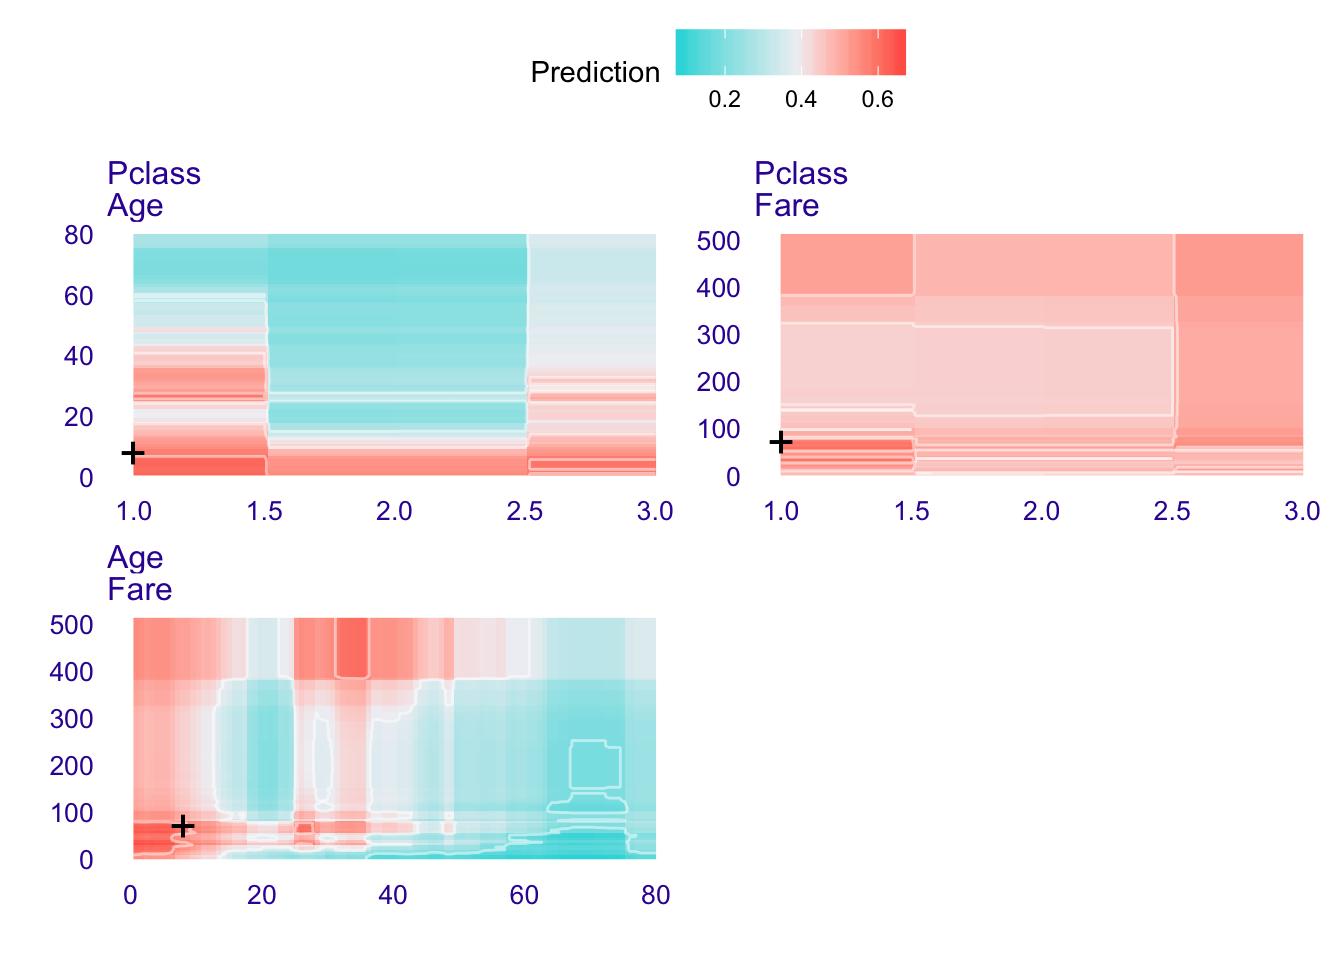
\includegraphics{PM_VEE_files/figure-latex/unnamed-chunk-9-1.pdf}

Add the \texttt{plot\_distributions\ =\ TRUE} argument to enrich model
response with additional information.

\begin{Shaded}
\begin{Highlighting}[]
\KeywordTok{plot}\NormalTok{(bd_rf, }\DataTypeTok{plot_distributions =} \OtherTok{TRUE}\NormalTok{) }
\end{Highlighting}
\end{Shaded}

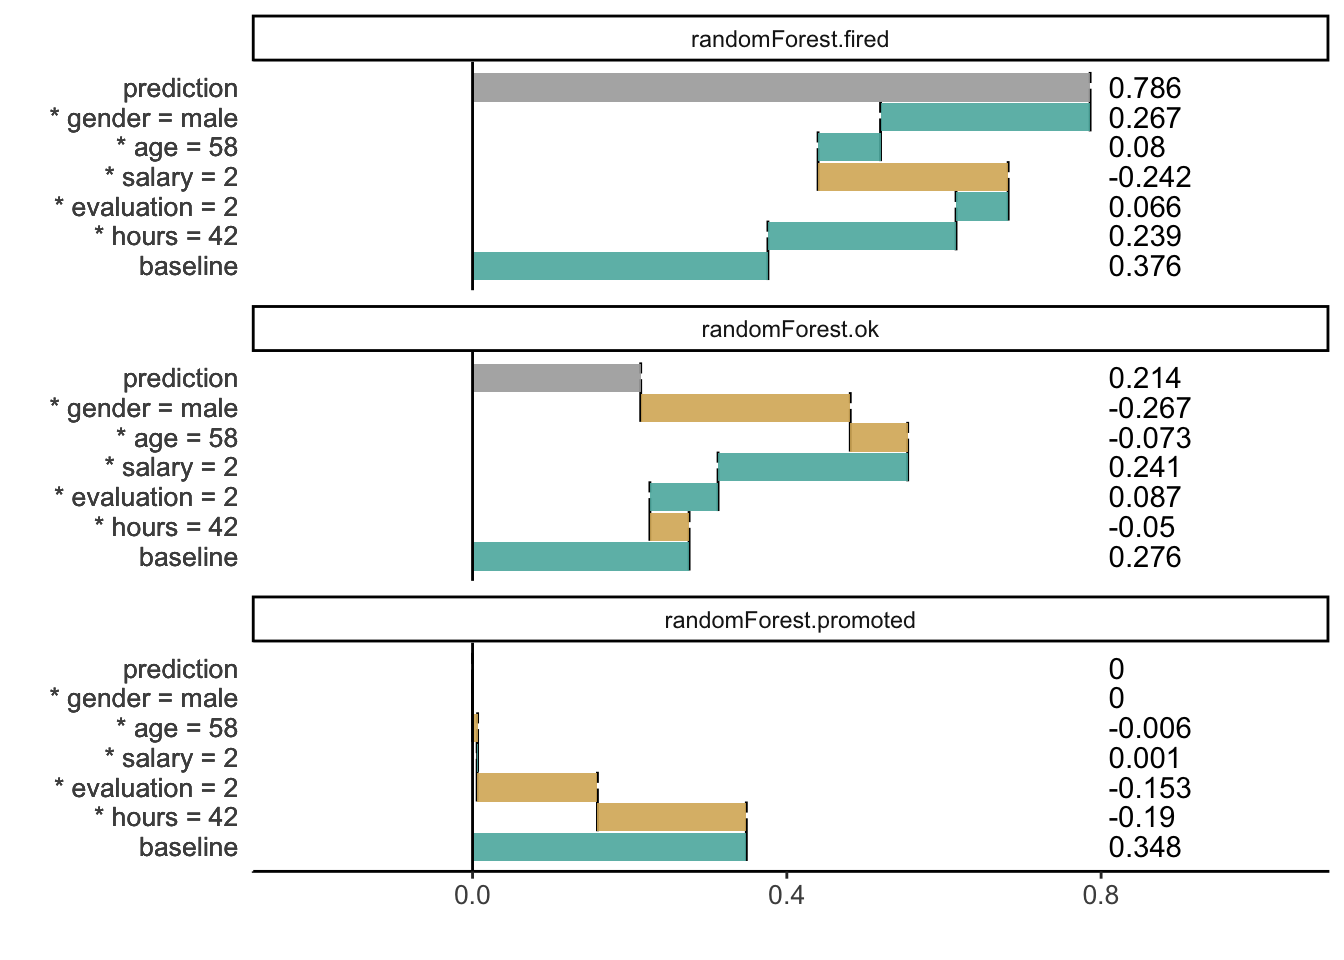
\includegraphics{PM_VEE_files/figure-latex/unnamed-chunk-10-1.pdf}

\hypertarget{sequential-variable-attribution-with-interactions}{%
\section{Sequential variable attribution with
interactions}\label{sequential-variable-attribution-with-interactions}}

In the Section \ref{breakDown} we presented model agnostic approach for
additive decomposition of a model prediction for a single observation.

For non-additive models the variables contributions depend on values of
other variables.

In this section we present an algorithm that identifies interactions
between pairs of variables and include such interactions in variable
decomposition plots. Here we present an algorithm for pairs of
variables, but it can be easily generalized to larger number of
variables.

\hypertarget{intuition-2}{%
\subsection{Intuition}\label{intuition-2}}

The key idea here is to identify interactions between variables. This
can be done in two steps.

\begin{enumerate}
\def\labelenumi{\arabic{enumi}.}
\tightlist
\item
  First we determine variable contributions for each variable
  independently.
\item
  Second, we calculate effect for pair of variables. If this effect is
  different than the sum of consecutive variables then it may be an
  interaction.
\end{enumerate}

TODO: easy example for interaction

\hypertarget{method-2}{%
\subsection{Method}\label{method-2}}

This algorithm is also composed out of two steps. In the first step
variables and pairs of variables are ordered in terms of their
importance, while in the second step the consecutive conditioning is
applied to ordered variables.

To determine an importance of variables and pairs of variables following
scores are being calculated.

For a single variable

\[
score_1(f, x^*, i) = \left| E [f(X)|X_i = x^*_i]  - E [f(X)]\right|
\] For pairs of variables

\[
score_2(f, x^*, (i,j)) = \left| E [f(X)|X_i = x^*_i, X_j = x^*_j] - E [f(X)|X_i = x^*_i] - E [f(X)| X_j = x^*_j]+ E [f(X)] \right|
\] Note that this is equivalent to

\[
score_2(f, x^*, (i,j)) = \left| E [f(X)|X_i = x^*_i, X_j = x^*_j] - score_1 (f, x^*, i) - score_1 (f, x^*, j) + baseline \right|
\] In other words the \(score_1(f, x^*, i)\) measures how much the
average model response changes if variable \(x_i\) is set to \(x_i^*\),
which is some index of local variable importance. On the other hand the
\(score_2(f, x^*, (i,j))\) measures how much the change is different
than additive composition of changes for \(x_i\) and \(x_j\), which is
some index of local interaction importance.

Note, that for additive models \(score_2(f, x^*, (i,j))\) shall be close
to zero. So the larger is this value the larger deviation from
additivness.

The second step of the algorithm is the sequential conditioning. In this
version in every new step we condition on a single variable of pair of
variables in an order determined by \(score_1\) and \(score_2\).

The complexity of the first step id \(O(p^2)\) where \(p\) stands for
the number of variables. The complexity of the second step is \(O(p)\).

\hypertarget{example-hire-or-fire-1}{%
\subsection{Example: Hire or Fire?}\label{example-hire-or-fire-1}}

Again, let us consider a HR dataset. The table below shows \(score_1\)
and \(score_2\) calculated for consecutive variables.

\begin{longtable}[]{@{}lrrr@{}}
\toprule
& Ei f(X) & score1 & score2\tabularnewline
\midrule
\endhead
hours & 0.616200 & 0.230614 &\tabularnewline
salary & 0.225528 & -0.160058 &\tabularnewline
age:gender & 0.516392 & & 0.146660\tabularnewline
salary:age & 0.266226 & & 0.062026\tabularnewline
salary:hours & 0.400206 & & -0.055936\tabularnewline
evaluation & 0.430994 & 0.045408 &\tabularnewline
hours:age & 0.635662 & & 0.040790\tabularnewline
salary:evaluation & 0.238126 & & -0.032810\tabularnewline
age & 0.364258 & -0.021328 &\tabularnewline
evaluation:hours & 0.677798 & & 0.016190\tabularnewline
salary:gender & 0.223292 & & -0.007710\tabularnewline
evaluation:age & 0.415688 & & 0.006022\tabularnewline
gender & 0.391060 & 0.005474 &\tabularnewline
hours:gender & 0.626478 & & 0.004804\tabularnewline
evaluation:gender & 0.433814 & & -0.002654\tabularnewline
\bottomrule
\end{longtable}

Once we determined the order, we can calculate sequential conditionings.
In the first step we condition over variable \texttt{hours}, then over
\texttt{salary}. The third position is occupied by interaction between
\texttt{age:gender} thus we add both variables to the conditioning

\begin{longtable}[]{@{}lrr@{}}
\toprule
variable & cumulative & contribution\tabularnewline
\midrule
\endhead
(Intercept) & 0.385586 & 0.385586\tabularnewline
* hours = 42 & 0.616200 & 0.230614\tabularnewline
* salary = 2 & 0.400206 & -0.215994\tabularnewline
* age:gender = 58:male & 0.796856 & 0.396650\tabularnewline
* evaluation = 2 & 0.778000 & -0.018856\tabularnewline
final\_prognosis & 0.778000 & 0.778000\tabularnewline
\bottomrule
\end{longtable}

\hypertarget{break-down-plots}{%
\subsection{Break Down Plots}\label{break-down-plots}}

Break Down Plots for interactions are similar in structure as plots for
single variables. The only difference is that in some rows pair of
variable is listed in a single row. See an example in Figure
\ref{BDPrice4}.

\begin{figure}

{\centering 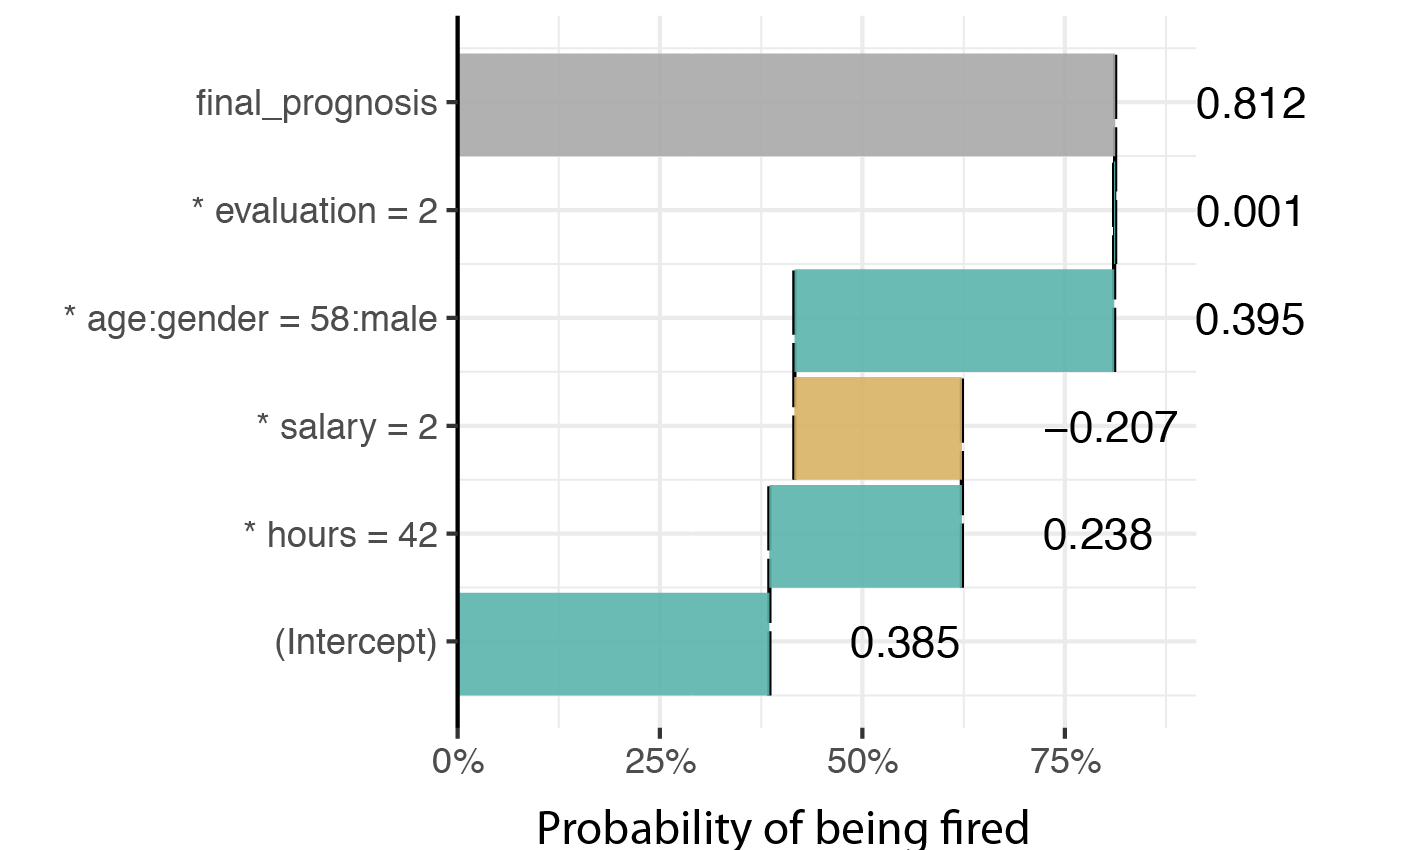
\includegraphics[width=0.7\linewidth]{figure/bd_inter_1} 

}

\caption{(fig:bdInter1) Break Down Plot for variable attrbution with interactions }\label{fig:bdInter1}
\end{figure}

\hypertarget{pros-and-cons-2}{%
\subsection{Pros and cons}\label{pros-and-cons-2}}

Break Down for interactions shares many features of Break Down for
single variables. Below we summarize unique strengths and weaknesses of
this approach.

\textbf{Pros}

\begin{itemize}
\tightlist
\item
  If interactions are present in the model, then additive contributions
  may be misleading. In such case the identification of interactions
  leads to better explanations.
\item
  Complexity of Break Down Algorithm is quadratic, what is not that bad
  if number of features is small or moderate.
\end{itemize}

\textbf{Cons}

\begin{itemize}
\tightlist
\item
  For large number of variables, the consideration of all interactions
  is both time consuming and sensitive to noise as the number of
  \(score_2\) scores grow faster than number of \(score_1\).
\end{itemize}

\hypertarget{code-snippets-for-r-1}{%
\subsection{Code snippets for R}\label{code-snippets-for-r-1}}

The algorithm for Break Down for Interactions is also implemented in the
\texttt{break\_down} function from \texttt{breakDown} package.

It is enough to set argument \texttt{check\_interactions\ =\ TRUE} to
identify interactions.

\textbf{Model preparation}

First a model needs to be trained.

\begin{Shaded}
\begin{Highlighting}[]
\KeywordTok{library}\NormalTok{(}\StringTok{"DALEX"}\NormalTok{)}
\KeywordTok{library}\NormalTok{(}\StringTok{"randomForest"}\NormalTok{)}
\NormalTok{model <-}\StringTok{ }\KeywordTok{randomForest}\NormalTok{(status }\OperatorTok{~}\StringTok{ }\NormalTok{gender }\OperatorTok{+}\StringTok{ }\NormalTok{age }\OperatorTok{+}\StringTok{ }\NormalTok{hours }\OperatorTok{+}\StringTok{ }\NormalTok{evaluation }\OperatorTok{+}\StringTok{ }\NormalTok{salary, }\DataTypeTok{data =}\NormalTok{ HR)}
\NormalTok{model}
\end{Highlighting}
\end{Shaded}

\begin{verbatim}
## 
## Call:
##  randomForest(formula = status ~ gender + age + hours + evaluation +      salary, data = HR) 
##                Type of random forest: classification
##                      Number of trees: 500
## No. of variables tried at each split: 2
## 
##         OOB estimate of  error rate: 27.11%
## Confusion matrix:
##          fired   ok promoted class.error
## fired     2276  380      199   0.2028021
## ok         524 1255      442   0.4349392
## promoted   197  385     2189   0.2100325
\end{verbatim}

Model exploration with the \texttt{breakDown} package is performed in
three steps.

\textbf{1. Create an explainer - wrapper around model and validation
data.}

Since all other functions work in a model agnostic fashion, first we
need to define a wrapper around the model. Here we are using the
\texttt{explain()} function from \texttt{DALEX} package.

\begin{Shaded}
\begin{Highlighting}[]
\NormalTok{explainer_rf_fired <-}\StringTok{ }\KeywordTok{explain}\NormalTok{(model,}
                 \DataTypeTok{data =}\NormalTok{ HR,}
                 \DataTypeTok{y =}\NormalTok{ HR}\OperatorTok{$}\NormalTok{status }\OperatorTok{==}\StringTok{ "fired"}\NormalTok{,}
                 \DataTypeTok{predict_function =} \ControlFlowTok{function}\NormalTok{(m,x) }\KeywordTok{predict}\NormalTok{(m,x, }\DataTypeTok{type =} \StringTok{"prob"}\NormalTok{)[,}\DecValTok{1}\NormalTok{],}
                 \DataTypeTok{label =} \StringTok{"fired"}\NormalTok{)}
\end{Highlighting}
\end{Shaded}

\textbf{2. Select an observation of interest.}

Break Down Plots decompose model prediction around a single observation.
Let's construct a data frame with corresponding values.

\begin{Shaded}
\begin{Highlighting}[]
\NormalTok{new_observation <-}\StringTok{ }\KeywordTok{data.frame}\NormalTok{(}\DataTypeTok{gender =} \KeywordTok{factor}\NormalTok{(}\StringTok{"male"}\NormalTok{, }\DataTypeTok{levels =} \KeywordTok{c}\NormalTok{(}\StringTok{"male"}\NormalTok{, }\StringTok{"female"}\NormalTok{)),}
                      \DataTypeTok{age =} \FloatTok{57.7}\NormalTok{,}
                      \DataTypeTok{hours =} \FloatTok{42.3}\NormalTok{,}
                      \DataTypeTok{evaluation =} \DecValTok{2}\NormalTok{,}
                      \DataTypeTok{salary =} \DecValTok{2}\NormalTok{)}

\KeywordTok{predict}\NormalTok{(model, new_observation, }\DataTypeTok{type =} \StringTok{"prob"}\NormalTok{)}
\end{Highlighting}
\end{Shaded}

\begin{verbatim}
##   fired    ok promoted
## 1 0.806 0.194        0
## attr(,"class")
## [1] "matrix" "votes"
\end{verbatim}

\textbf{3. Calculate Break Down decomposition}

The \texttt{break\_down()} function calculates Break Down contributions
for a selected model around a selected observation.

Note that \texttt{check\_interactions\ =\ TRUE} is needed to identify
interactions.

The result from \texttt{break\_down()} function is a data frame with
variable attributions.

\begin{Shaded}
\begin{Highlighting}[]
\KeywordTok{library}\NormalTok{(}\StringTok{"breakDown"}\NormalTok{)}
\NormalTok{bd_rf <-}\StringTok{ }\KeywordTok{break_down}\NormalTok{(explainer_rf_fired,}
\NormalTok{                 new_observation,}
                 \DataTypeTok{check_interactions =} \OtherTok{TRUE}\NormalTok{)}

\NormalTok{bd_rf}
\end{Highlighting}
\end{Shaded}

\begin{verbatim}
##                        contribution
## (Intercept)                   0.375
## * hours = 42                  0.237
## * salary = 2                 -0.204
## * age:gender = 58:male        0.396
## * evaluation = 2              0.001
## final_prognosis               0.806
## baseline:  0
\end{verbatim}

The generic \texttt{plot()} function creates a Break Down plots.

\begin{Shaded}
\begin{Highlighting}[]
\KeywordTok{plot}\NormalTok{(bd_rf) }
\end{Highlighting}
\end{Shaded}

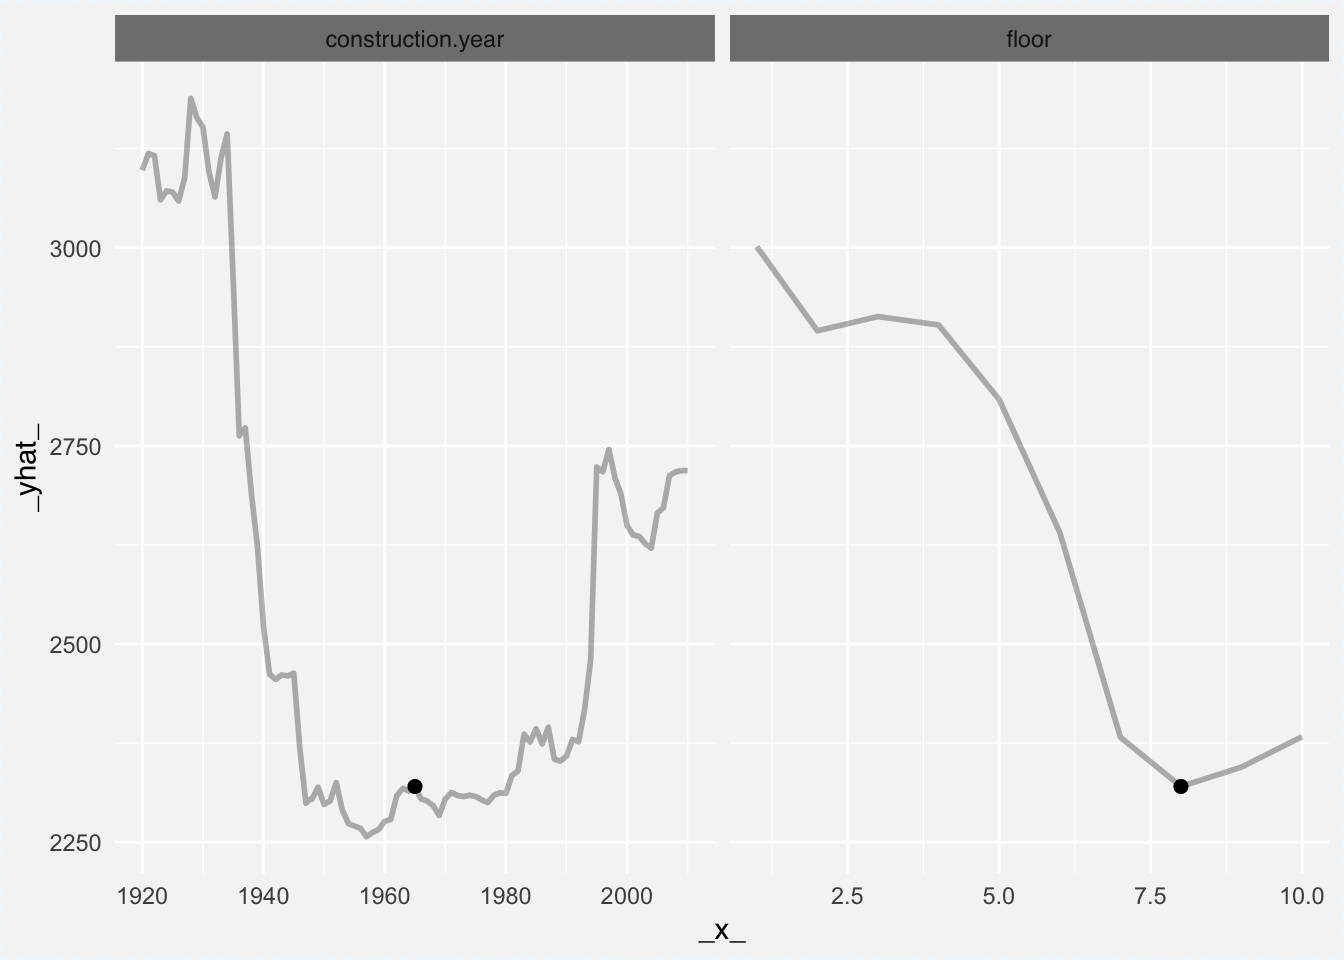
\includegraphics{PM_VEE_files/figure-latex/unnamed-chunk-15-1.pdf}

\hypertarget{shapley}{%
\section{Average variable attributions}\label{shapley}}

In the Section \ref{modelAgnosticAttribution} we show the problem
related to the ordering of variables. In the Section \ref{breakDown} we
show an approach in which the ordering was determined based on single
step assessment of variable importance.

In this section we introduce other, very popular approach for additive
variable attribution. The problem of contributions that depends on the
variable ordering is solved by averaging over all possible orderings.

This method is motivated with results in cooperative game theory and was
first introduced in \citep{Strumbelj2014}. Wide adoption of this method
comes with a NIPS 2017 paper \citep{SHAP} and python library SHAP
\texttt{https://github.com/slundberg/shap}. Authors of the SHAP method
introduced also efficient algorithm for tree-based models, see
\citep{TreeSHAP}.

\hypertarget{intuition-3}{%
\subsection{Intuition}\label{intuition-3}}

Since in sequential attribution effect depends on the ordering. Here the
idea is to average across all possible orderings.

TODO: a nice example

\hypertarget{method-3}{%
\subsection{Method}\label{method-3}}

The name \emph{Shapley Values} comes from the solution in cooperative
game theory attributed to Lloyd Shapley. The original problem was to
assess how important is each player to the overall cooperation, and what
payoff can he or she reasonably expect from the coalition?
\citep{shapleybook1952}

In the context of model interpretability the payoff is the average model
response while the players are the variables in the conditioning. Then
Formula for variable contributions is following.

\[
v(f, x^*, i) = \frac 1{|P|}\sum_{S \subseteq P\setminus \{i\}}  {{|P|-1}\choose{|S|}}^{-1} \left(E [f(X) | X_{S \cup \{i\}} = x^*_{S \cup \{i\}}] - E [f(X) | X_{S} = x^*_{S}]\right)
\] where \(P = \{1, \ldots, p\}\) is the set of all variables. The
intuition beyond this contribution is following. We consider all
possible orderings of variables (yes, there is \(2^p\) of them) and
calculate the contribution of variable \(i\) as an average from
contributions calculated in particular orderings.

The part
\(E[f(X) | X_{S \cup \{i\}} = x^*_{S \cup \{i\}}] - E [f(X) | X_{S} = x^*_{S}]\)
is the contribution of variable \(i\) which is introduces after
variables from \(S\).

Time complexity of this method is \(O(2^p)\) where \(p\) stands for the
number of variables. Such complexity makes this method impractical for
most cases. Fortunately it is enough to assess this value.
\citep{Strumbelj2014} proposed to use sampling. \citep{TreeSHAP}
proposed fast implementations for tree based ensembles.

\hypertarget{example-hire-or-fire-2}{%
\subsection{Example: Hire or Fire?}\label{example-hire-or-fire-2}}

\hypertarget{pros-and-cons-3}{%
\subsection{Pros and cons}\label{pros-and-cons-3}}

Shapley Values give a uniform approach to decompose model prediction
into parts that can be attributed additively to variables. Below we
summarize key strengths and weaknesses of this approach.

\textbf{Pros}

\begin{itemize}
\tightlist
\item
  There is a nice theory based on cooperative games.
\item
  \citep{SHAP} shows that this method unifies different approaches to
  additive features attribution.
\item
  There is efficient implementation available for Python.
\item
  \citep{SHAP} shows more desired properties of this method, like
  symmetry or additivity.
\end{itemize}

\textbf{Cons}

\begin{itemize}
\tightlist
\item
  The exact calculation of Shapley values is time consuming.
\item
  If the model is not additive, then the Shaply scores may be
  misleading. And there is no way to determine if model is far from
  additiveness.
\end{itemize}

Note that fully additive model solutions presented in sections
\ref{modelAgnosticAttribution}, \ref{breakDown} and \ref{shapley} lead
to same variable contributions.

\hypertarget{code-snippets-for-r-2}{%
\subsection{Code snippets for R}\label{code-snippets-for-r-2}}

In this section we will present an example based on the \texttt{HR}
dataset and Random Forest model \citep{R-randomForest}. See the Section
\ref{HRdataset} for more details.

\begin{Shaded}
\begin{Highlighting}[]
\KeywordTok{library}\NormalTok{(}\StringTok{"DALEX"}\NormalTok{)}
\KeywordTok{library}\NormalTok{(}\StringTok{"randomForest"}\NormalTok{)}
\NormalTok{model_rf <-}\StringTok{ }\KeywordTok{randomForest}\NormalTok{(status }\OperatorTok{~}\StringTok{ }\NormalTok{gender }\OperatorTok{+}\StringTok{ }\NormalTok{age }\OperatorTok{+}\StringTok{ }\NormalTok{hours }\OperatorTok{+}\StringTok{ }\NormalTok{evaluation }\OperatorTok{+}\StringTok{ }\NormalTok{salary, }\DataTypeTok{data =}\NormalTok{ HR)}
\end{Highlighting}
\end{Shaded}

Here we use the \texttt{iml} package, see more examples in
\citep{imlPackage}.

\begin{Shaded}
\begin{Highlighting}[]
\KeywordTok{library}\NormalTok{(}\StringTok{"iml"}\NormalTok{)}
\NormalTok{explainer_rf =}\StringTok{ }\NormalTok{Predictor}\OperatorTok{$}\KeywordTok{new}\NormalTok{(model_rf, }\DataTypeTok{data =}\NormalTok{ HR, }\DataTypeTok{type=}\StringTok{"prob"}\NormalTok{)}
\end{Highlighting}
\end{Shaded}

Explanations for a new observation.

\begin{Shaded}
\begin{Highlighting}[]
\NormalTok{new_observation <-}\StringTok{ }\KeywordTok{data.frame}\NormalTok{(}\DataTypeTok{gender =} \KeywordTok{factor}\NormalTok{(}\StringTok{"male"}\NormalTok{, }\DataTypeTok{levels =} \KeywordTok{c}\NormalTok{(}\StringTok{"male"}\NormalTok{, }\StringTok{"female"}\NormalTok{)),}
                      \DataTypeTok{age =} \FloatTok{57.7}\NormalTok{,}
                      \DataTypeTok{hours =} \FloatTok{42.3}\NormalTok{,}
                      \DataTypeTok{evaluation =} \DecValTok{2}\NormalTok{,}
                      \DataTypeTok{salary =} \DecValTok{2}\NormalTok{,}
                      \DataTypeTok{status =} \KeywordTok{factor}\NormalTok{(}\StringTok{"fired"}\NormalTok{))}

\NormalTok{shapley =}\StringTok{ }\NormalTok{Shapley}\OperatorTok{$}\KeywordTok{new}\NormalTok{(explainer_rf, }\DataTypeTok{x.interest =}\NormalTok{ new_observation)}
\NormalTok{shapley}
\end{Highlighting}
\end{Shaded}

\begin{verbatim}
## Interpretation method:  Shapley 
## Predicted value: 0.790000, Average prediction: 0.375134 (diff = 0.414866) Predicted value: 0.206000, Average prediction: 0.275333 (diff = -0.069333) Predicted value: 0.004000, Average prediction: 0.349532 (diff = -0.345532)
## 
## Analysed predictor: 
## Prediction task: unknown 
## 
## 
## Analysed data:
## Sampling from data.frame with 7847 rows and 6 columns.
## 
## Head of results:
##      feature class      phi     phi.var feature.value
## 1     gender fired  0.15264 0.078219788   gender=male
## 2        age fired  0.14534 0.076510388      age=57.7
## 3      hours fired  0.27040 0.109291071    hours=42.3
## 4 evaluation fired  0.01490 0.007215545  evaluation=2
## 5     salary fired -0.14540 0.061668242      salary=2
## 6     status fired  0.00000 0.000000000  status=fired
\end{verbatim}

And the plot with Shapley attributions.

\begin{Shaded}
\begin{Highlighting}[]
\KeywordTok{plot}\NormalTok{(shapley)}
\end{Highlighting}
\end{Shaded}

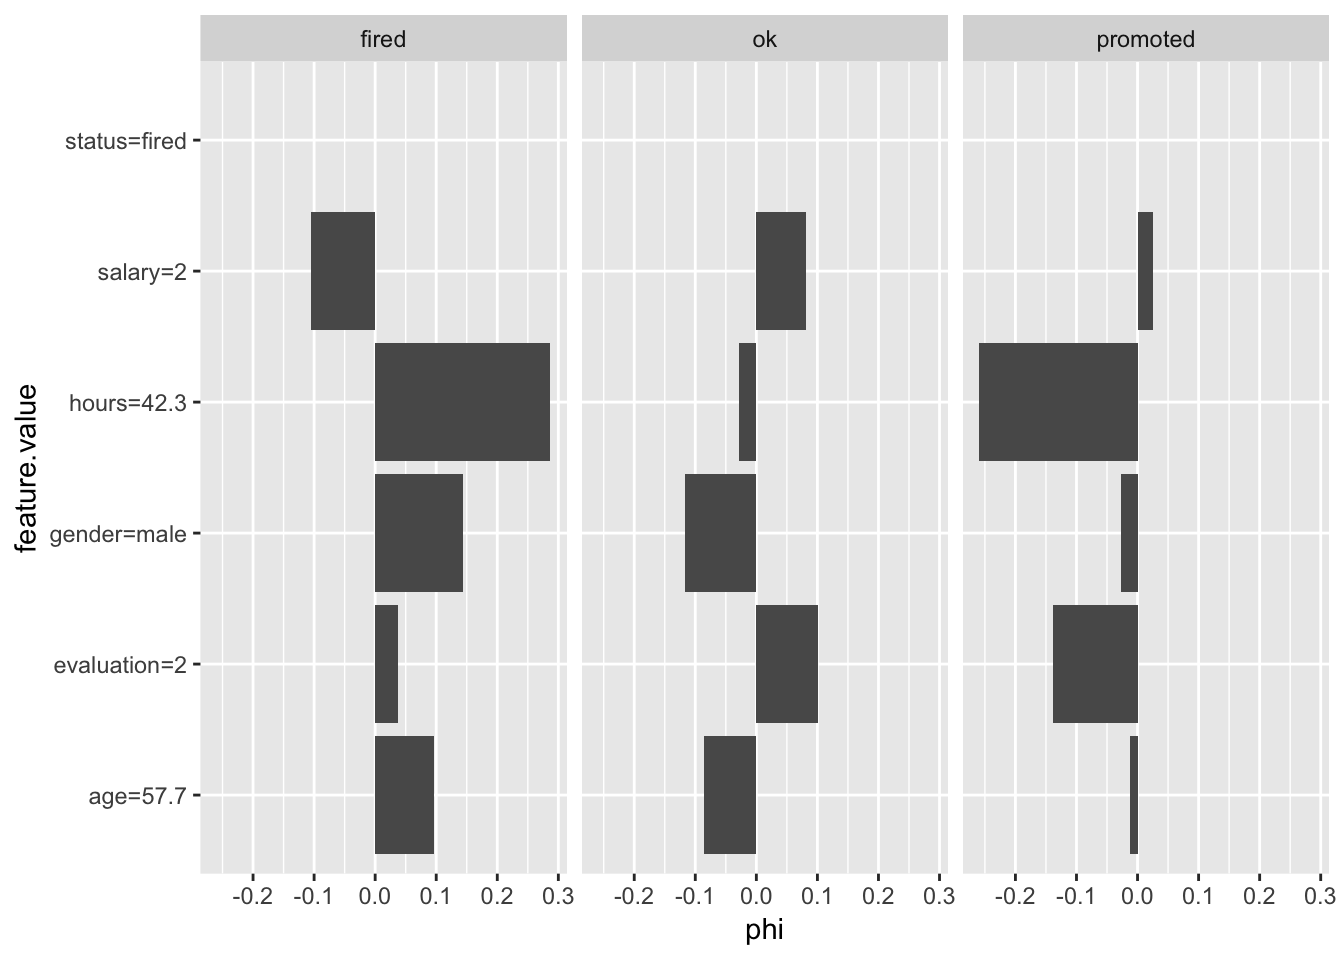
\includegraphics{PM_VEE_files/figure-latex/unnamed-chunk-19-1.pdf}

See more examples for \texttt{iml} package in the \citep{molnar} book.

\hypertarget{LIME}{%
\section{Local approximations with white-box model}\label{LIME}}

A different approach to explanations of a single observations is through
surrogate models. Models that easy to understand and are similar to
black box model around the point of interest.

Variable attribution methods, that were presented in the Section
\ref{breakDown} are not interested in the local curvature of the model.
They rather compare model prediction against average model prediction
and they use probability structure of the dataset.

The complementary approach would be to directly explore information
about model curvature around point of interest. In the section
\ref{ceterisParibus} we introduced Ceteris Paribus tool for such what-if
analysis. But the limitation of ceteris Paribus pltos is that they
explore changes along single dimension or pairs of dimensions.

In this section we describe an another approach based on local
approximations with white-box models. This approach will also
investigate local curvature of the model but indirectly, through
surrogate white-box models.

The most known method from this class if LIME (Local Interpretable
Model-Agnostic Explanations), introduced in the paper \emph{Why Should I
Trust You?: Explaining the Predictions of Any Classifier} \citep{lime}.
This methods and it's clones are now implemented in various R and python
packages, see for example \citep{R-lime}, \citep{R-live} or
\citep{R-iml}.

\hypertarget{intuition-4}{%
\subsection{Intuition}\label{intuition-4}}

\hypertarget{method-4}{%
\subsection{Method}\label{method-4}}

The LIME method, and its clones, has following properties:

\begin{itemize}
\tightlist
\item
  \emph{model-agnostic}, they do not imply any assumptions on model
  structure,
\item
  \emph{interpretable representation}, model input is transformed into a
  feature space that is easier to understand. One of applications comes
  from image data, single pixels are not easy to interpret, thus the
  LIME method decompose image into a series of super pixels, that are
  easier to interpret to humans,
\item
  \emph{local fidelity} means that the explanations shall be locally
  well fitted to the black-box model.
\end{itemize}

Therefore the objective is to find a local model \(M^L\) that
approximates the black box model \(f\) in the point \(x^*\). As a
solution the penalized loss function is used. The white-box model that
is used for explanations satisfies following condition.

\[
M^L(x^*) = \arg \min_{g \in G} L(f, g, \Pi_{x^*}) + \Omega (g) 
\] where \(G\) is a family of white box models (e.g.~linear models),
\(\Pi_{x^*}\) is neighbourhood of \(x^*\) and \(\Omega\) stands for
model complexity.

\begin{figure}

{\centering 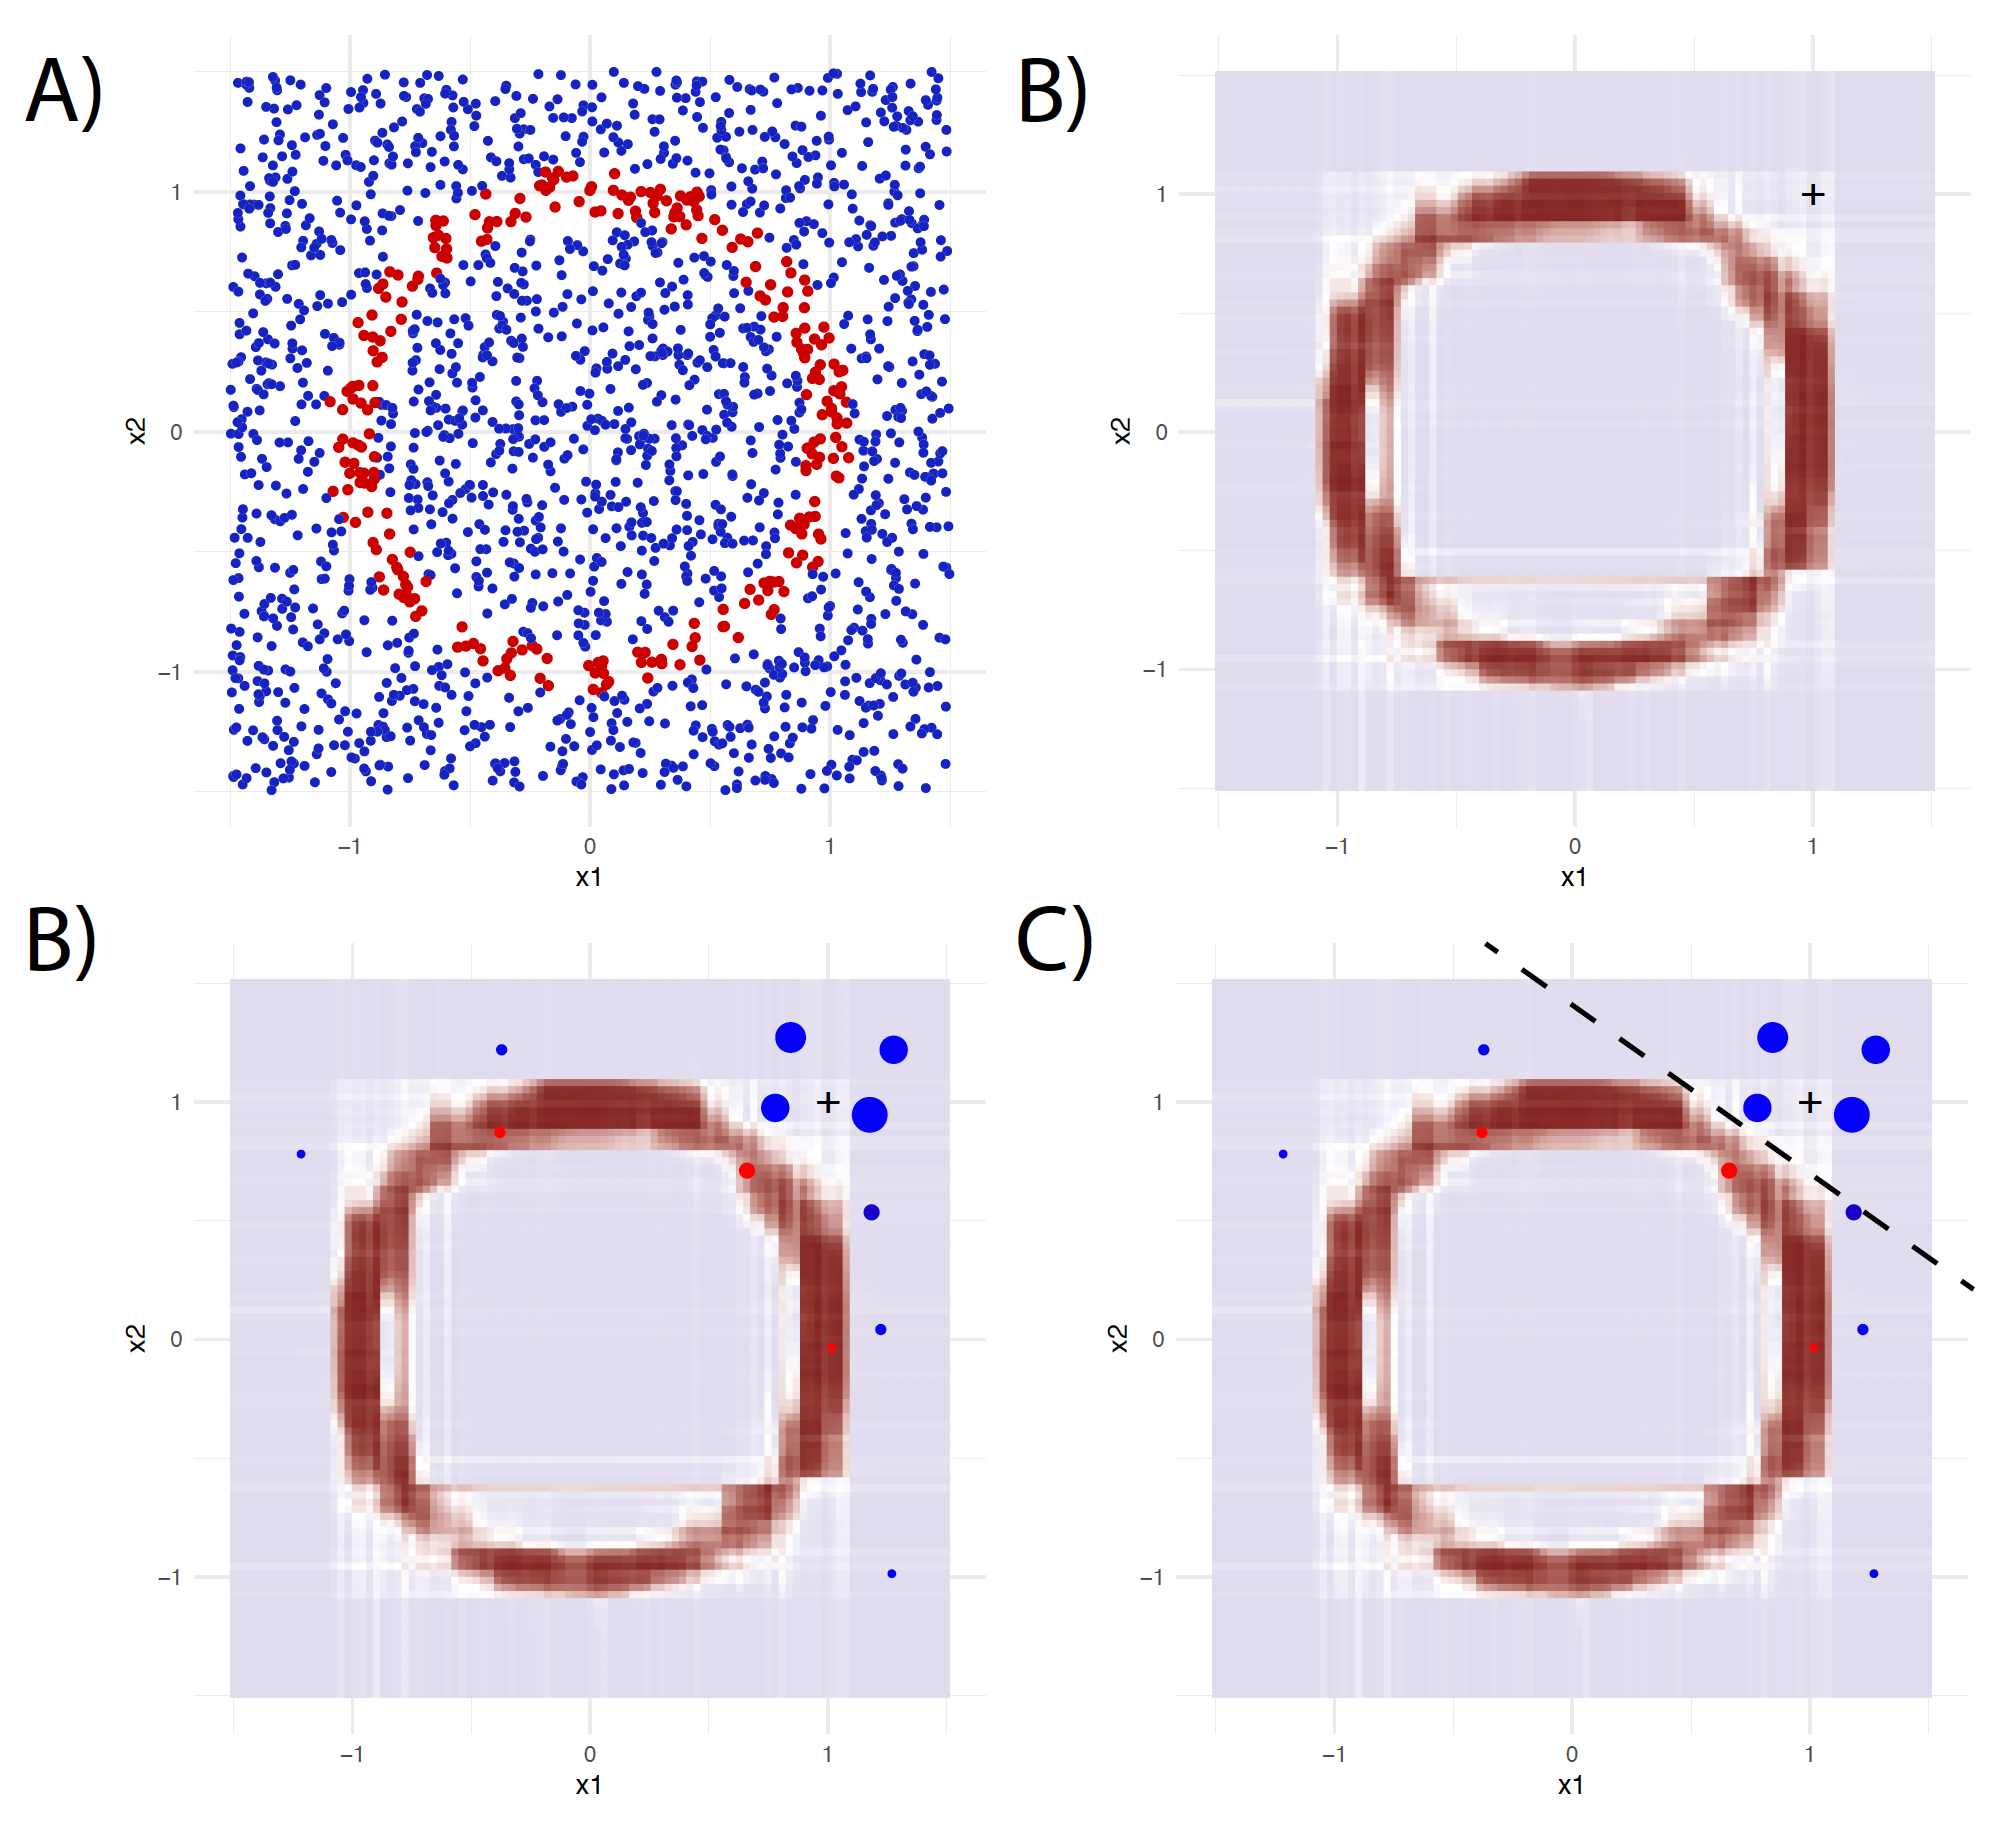
\includegraphics[width=0.7\linewidth]{figure/circle_4panels} 

}

\caption{(fig:LIME1) A schematic idea behind local model approximations. Panel A shows training data, colors correspond to classess. Panel B showhs results fom the Random Forest model, whis is where the algorithm starts. Panel C shows new data sampled around the point of interest. Their color correspond to model response. Panel D shows fitted linear model that approximated the random forest model around point of interest}\label{fig:LIME1}
\end{figure}

The algorithm is composed from three steps:

\begin{itemize}
\tightlist
\item
  Identification of interpretable data representations,
\item
  Local sampling around the point of interest,
\item
  Fitting a white box model in this neighbouhood
\end{itemize}

\textbf{Identification of interpretable data representations}

For image data, single pixel is not an interpretable feature. In this
step the input space of the model is transformed to input space that is
easier to understand for human. The image may be decomposed into parts
and represented as presence/absence of some part of an image.

\textbf{Local sampling around the point of interest}

Once the interpretable data representation is identified, then the
neighbourhood around point of interest needs to be explored.

\textbf{Fitting a white box model in this neighbouhood}

Any model that is easy to interpret may be fitted to this data, like
decision tree or rule based system. However in practice the most common
family of models are linear models.

\hypertarget{example-hire-or-fire-3}{%
\subsection{Example: Hire or Fire?}\label{example-hire-or-fire-3}}

\hypertarget{pros-and-cons-4}{%
\subsection{Pros and cons}\label{pros-and-cons-4}}

Local approximations are model agnostic, can be applied to any
predictive model. Below we summarize key strengths and weaknesses of
this approach.

\textbf{Pros}

\begin{itemize}
\tightlist
\item
  This method is highly adopted in text analysis and image analysis, in
  part thanks to the interpretable data representations.
\item
  The intuition behind the model is straightforward
\item
  Model explanations are sparse, thus only small number of features is
  used
\end{itemize}

\textbf{Cons}

\begin{itemize}
\tightlist
\item
  For continuous variables and tabular data it is not that easy to find
  interpretable representations
\item
  The black-box model approximated the data and the white box model
  approximates the black box model. We do not have control over the
  quality of local fit of the white box model, thus the surrogate model
  may be misleading.
\item
  Due to the \emph{curse of dimensionality}, for high dimensional space
  points are sparse.
\end{itemize}

\hypertarget{code-snippets-for-r-3}{%
\subsection{Code snippets for R}\label{code-snippets-for-r-3}}

In this section we present example application of \texttt{lime}
\citep{R-lime} and \texttt{live} \citep{R-live} packages. Note that this
method is also implemented in \texttt{iml} \citep{R-iml} and other
packages. These pacakages differ in some details and also results in
different explanations.

\textbf{Model preparation}

In this section we will present examples based on the \texttt{HR}
dataset. See the Section \ref{HRdataset} for more details.

\begin{Shaded}
\begin{Highlighting}[]
\KeywordTok{library}\NormalTok{(}\StringTok{"DALEX"}\NormalTok{)}
\KeywordTok{head}\NormalTok{(HR)}
\end{Highlighting}
\end{Shaded}

\begin{verbatim}
##   gender      age    hours evaluation salary   status
## 1   male 32.58267 41.88626          3      1    fired
## 2 female 41.21104 36.34339          2      5    fired
## 3   male 37.70516 36.81718          3      0    fired
## 4 female 30.06051 38.96032          3      2    fired
## 5   male 21.10283 62.15464          5      3 promoted
## 6   male 40.11812 69.53973          2      0    fired
\end{verbatim}

The problem here is to predict average price for square meter for an
apartment. Let's build a random forest model with \texttt{randomForest}
package \citep{R-randomForest}.

\begin{Shaded}
\begin{Highlighting}[]
\KeywordTok{library}\NormalTok{(}\StringTok{"randomForest"}\NormalTok{)}
\NormalTok{rf_model <-}\StringTok{ }\KeywordTok{randomForest}\NormalTok{(status }\OperatorTok{~}\StringTok{ }\NormalTok{gender }\OperatorTok{+}\StringTok{ }\NormalTok{age }\OperatorTok{+}\StringTok{ }\NormalTok{hours }\OperatorTok{+}\StringTok{ }\NormalTok{evaluation }\OperatorTok{+}\StringTok{ }\NormalTok{salary, }\DataTypeTok{data =}\NormalTok{ HR)}
\NormalTok{rf_model}
\end{Highlighting}
\end{Shaded}

\begin{verbatim}
## 
## Call:
##  randomForest(formula = status ~ gender + age + hours + evaluation +      salary, data = HR) 
##                Type of random forest: classification
##                      Number of trees: 500
## No. of variables tried at each split: 2
## 
##         OOB estimate of  error rate: 27.44%
## Confusion matrix:
##          fired   ok promoted class.error
## fired     2276  382      197   0.2028021
## ok         539 1250      432   0.4371905
## promoted   205  398     2168   0.2176110
\end{verbatim}

\begin{Shaded}
\begin{Highlighting}[]
\NormalTok{new_observation <-}\StringTok{ }\KeywordTok{data.frame}\NormalTok{(}\DataTypeTok{gender =} \KeywordTok{factor}\NormalTok{(}\StringTok{"male"}\NormalTok{, }\DataTypeTok{levels =} \KeywordTok{c}\NormalTok{(}\StringTok{"male"}\NormalTok{, }\StringTok{"female"}\NormalTok{)),}
                      \DataTypeTok{age =} \FloatTok{57.7}\NormalTok{,}
                      \DataTypeTok{hours =} \FloatTok{42.3}\NormalTok{,}
                      \DataTypeTok{evaluation =} \DecValTok{2}\NormalTok{,}
                      \DataTypeTok{salary =} \DecValTok{2}\NormalTok{)}

\KeywordTok{predict}\NormalTok{(rf_model, new_observation, }\DataTypeTok{type =} \StringTok{"prob"}\NormalTok{)}
\end{Highlighting}
\end{Shaded}

\begin{verbatim}
##   fired   ok promoted
## 1  0.78 0.22        0
## attr(,"class")
## [1] "matrix" "votes"
\end{verbatim}

\hypertarget{the-lime-pacakge}{%
\subsubsection{\texorpdfstring{\textbf{The lime
pacakge}}{The lime pacakge}}\label{the-lime-pacakge}}

\begin{Shaded}
\begin{Highlighting}[]
\KeywordTok{library}\NormalTok{(}\StringTok{"lime"}\NormalTok{)}
\NormalTok{model_type.randomForest <-}\StringTok{ }\ControlFlowTok{function}\NormalTok{(x, ...) }\StringTok{"classification"}
\NormalTok{lime_rf <-}\StringTok{ }\KeywordTok{lime}\NormalTok{(HR[,}\DecValTok{1}\OperatorTok{:}\DecValTok{5}\NormalTok{], rf_model)}
\NormalTok{explanations <-}\StringTok{ }\NormalTok{lime}\OperatorTok{::}\KeywordTok{explain}\NormalTok{(new_observation[,}\DecValTok{1}\OperatorTok{:}\DecValTok{5}\NormalTok{], lime_rf, }\DataTypeTok{n_labels =} \DecValTok{3}\NormalTok{, }\DataTypeTok{n_features =} \DecValTok{3}\NormalTok{)}
\NormalTok{explanations}
\end{Highlighting}
\end{Shaded}

\begin{verbatim}
##       model_type case    label label_prob  model_r2 model_intercept
## 1 classification    1    fired       0.78 0.1280528       0.2560933
## 2 classification    1    fired       0.78 0.1280528       0.2560933
## 3 classification    1    fired       0.78 0.1280528       0.2560933
## 4 classification    1       ok       0.22 0.1300045       0.1927029
## 5 classification    1       ok       0.22 0.1300045       0.1927029
## 6 classification    1       ok       0.22 0.1300045       0.1927029
## 7 classification    1 promoted       0.00 0.2804175       0.5215667
## 8 classification    1 promoted       0.00 0.2804175       0.5215667
## 9 classification    1 promoted       0.00 0.2804175       0.5215667
##   model_prediction    feature feature_value feature_weight
## 1       0.65255924        age          57.7     0.02280602
## 2       0.65255924      hours          42.3     0.26315207
## 3       0.65255924 evaluation           2.0     0.11050785
## 4       0.45319767     gender           2.0    -0.01451984
## 5       0.45319767 evaluation           2.0     0.20570353
## 6       0.45319767     salary           2.0     0.06931111
## 7       0.00869987        age          57.7     0.00320708
## 8       0.00869987 evaluation           2.0    -0.31464457
## 9       0.00869987      hours          42.3    -0.20142934
##           feature_desc                      data       prediction
## 1           50.0 < age 2.0, 57.7, 42.3, 2.0, 2.0 0.78, 0.22, 0.00
## 2 37.6 < hours <= 46.3 2.0, 57.7, 42.3, 2.0, 2.0 0.78, 0.22, 0.00
## 3      evaluation <= 3 2.0, 57.7, 42.3, 2.0, 2.0 0.78, 0.22, 0.00
## 4        gender = male 2.0, 57.7, 42.3, 2.0, 2.0 0.78, 0.22, 0.00
## 5      evaluation <= 3 2.0, 57.7, 42.3, 2.0, 2.0 0.78, 0.22, 0.00
## 6      1 < salary <= 2 2.0, 57.7, 42.3, 2.0, 2.0 0.78, 0.22, 0.00
## 7           50.0 < age 2.0, 57.7, 42.3, 2.0, 2.0 0.78, 0.22, 0.00
## 8      evaluation <= 3 2.0, 57.7, 42.3, 2.0, 2.0 0.78, 0.22, 0.00
## 9 37.6 < hours <= 46.3 2.0, 57.7, 42.3, 2.0, 2.0 0.78, 0.22, 0.00
\end{verbatim}

\begin{Shaded}
\begin{Highlighting}[]
\KeywordTok{plot_features}\NormalTok{(explanations)}
\end{Highlighting}
\end{Shaded}

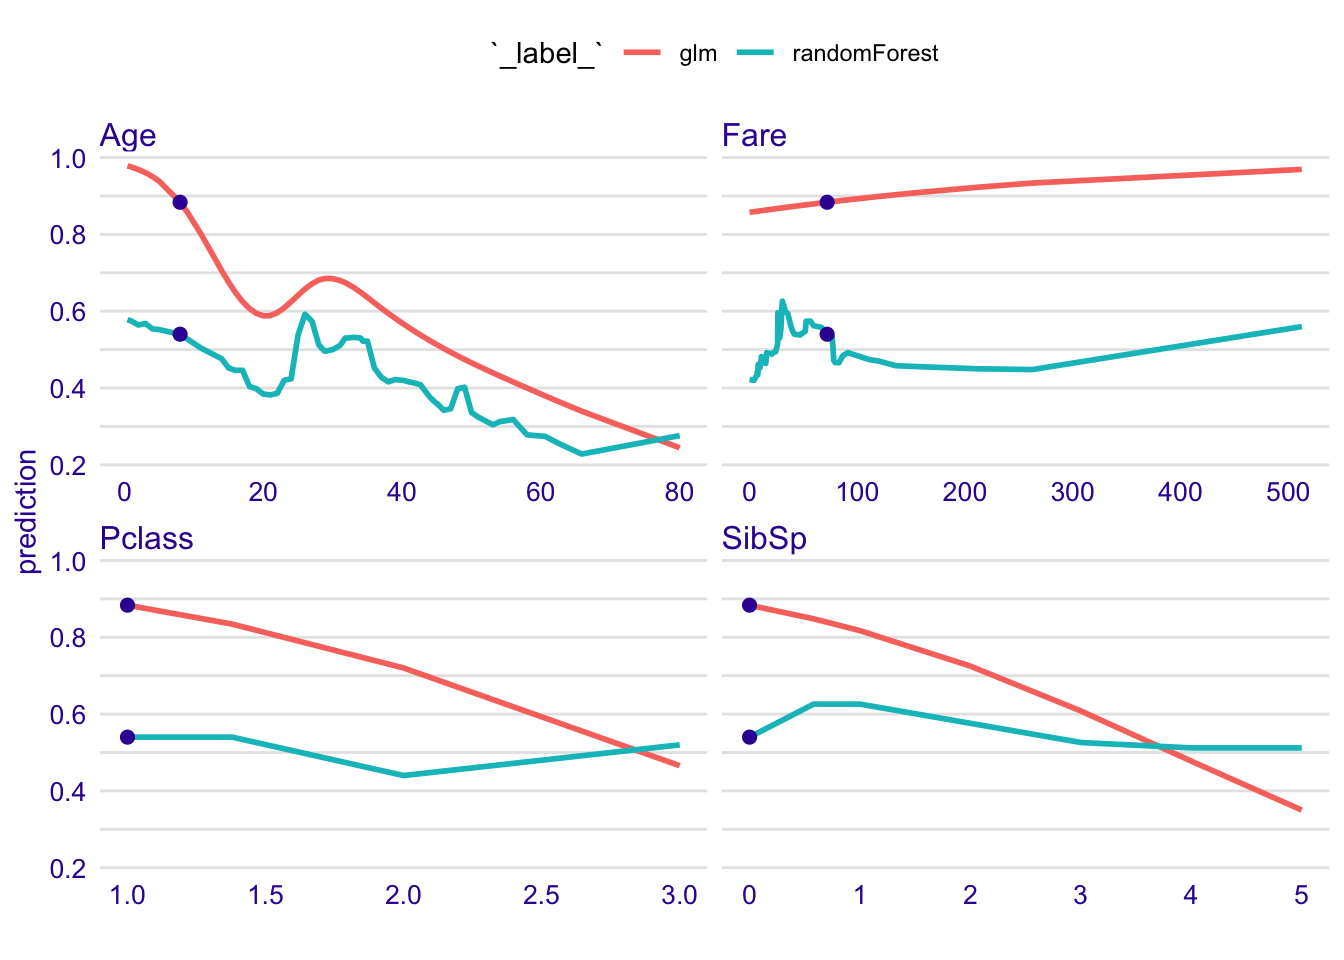
\includegraphics{PM_VEE_files/figure-latex/unnamed-chunk-24-1.pdf}

\hypertarget{the-live-package}{%
\subsubsection{\texorpdfstring{\textbf{The live
package}}{The live package}}\label{the-live-package}}

\begin{Shaded}
\begin{Highlighting}[]
\KeywordTok{library}\NormalTok{(}\StringTok{"live"}\NormalTok{)}

\NormalTok{new_observation}\OperatorTok{$}\NormalTok{status <-}\StringTok{ "fired"}
\NormalTok{explainer_rf_fired <-}\StringTok{ }\KeywordTok{explain}\NormalTok{(rf_model,}
                 \DataTypeTok{data =}\NormalTok{ HR,}
                 \DataTypeTok{y =}\NormalTok{ HR}\OperatorTok{$}\NormalTok{status }\OperatorTok{==}\StringTok{ "fired"}\NormalTok{,}
                 \DataTypeTok{predict_function =} \ControlFlowTok{function}\NormalTok{(m,x) }\KeywordTok{predict}\NormalTok{(m,x, }\DataTypeTok{type =} \StringTok{"prob"}\NormalTok{)[,}\DecValTok{1}\NormalTok{],}
                 \DataTypeTok{label =} \StringTok{"fired"}\NormalTok{)}

\NormalTok{local_model <-}\StringTok{ }\KeywordTok{local_approximation}\NormalTok{(explainer_rf_fired, new_observation, }
                    \DataTypeTok{target_variable_name =} \StringTok{"status"}\NormalTok{, }\DataTypeTok{n_new_obs =} \DecValTok{500}\NormalTok{)}

\NormalTok{local_model}
\end{Highlighting}
\end{Shaded}

\begin{verbatim}
## Dataset: 
##  Observations:  500 
##  Variables:  6 
##  Response variable:  status 
## Explanation model: 
##  Name:  regr.lm 
##  Variable selection wasn't performed 
##  Weights present in the explanation model 
##  R-squared: 0.977
\end{verbatim}

\begin{Shaded}
\begin{Highlighting}[]
\KeywordTok{plot}\NormalTok{(local_model)}
\end{Highlighting}
\end{Shaded}

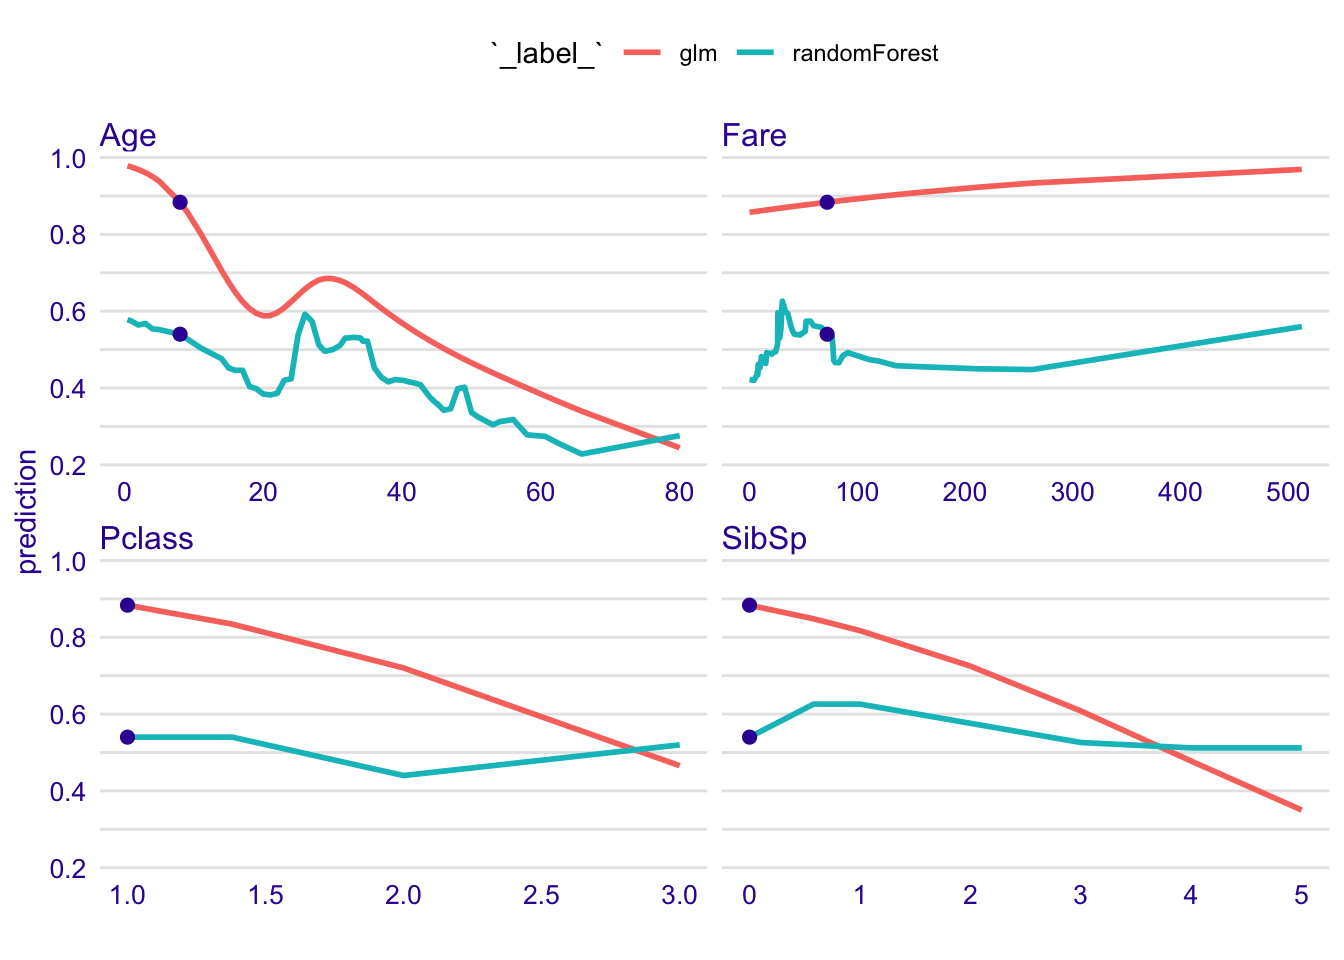
\includegraphics{PM_VEE_files/figure-latex/unnamed-chunk-25-1.pdf}

\begin{Shaded}
\begin{Highlighting}[]
\KeywordTok{plot}\NormalTok{(local_model, }\DataTypeTok{type =} \StringTok{"forest"}\NormalTok{)}
\end{Highlighting}
\end{Shaded}

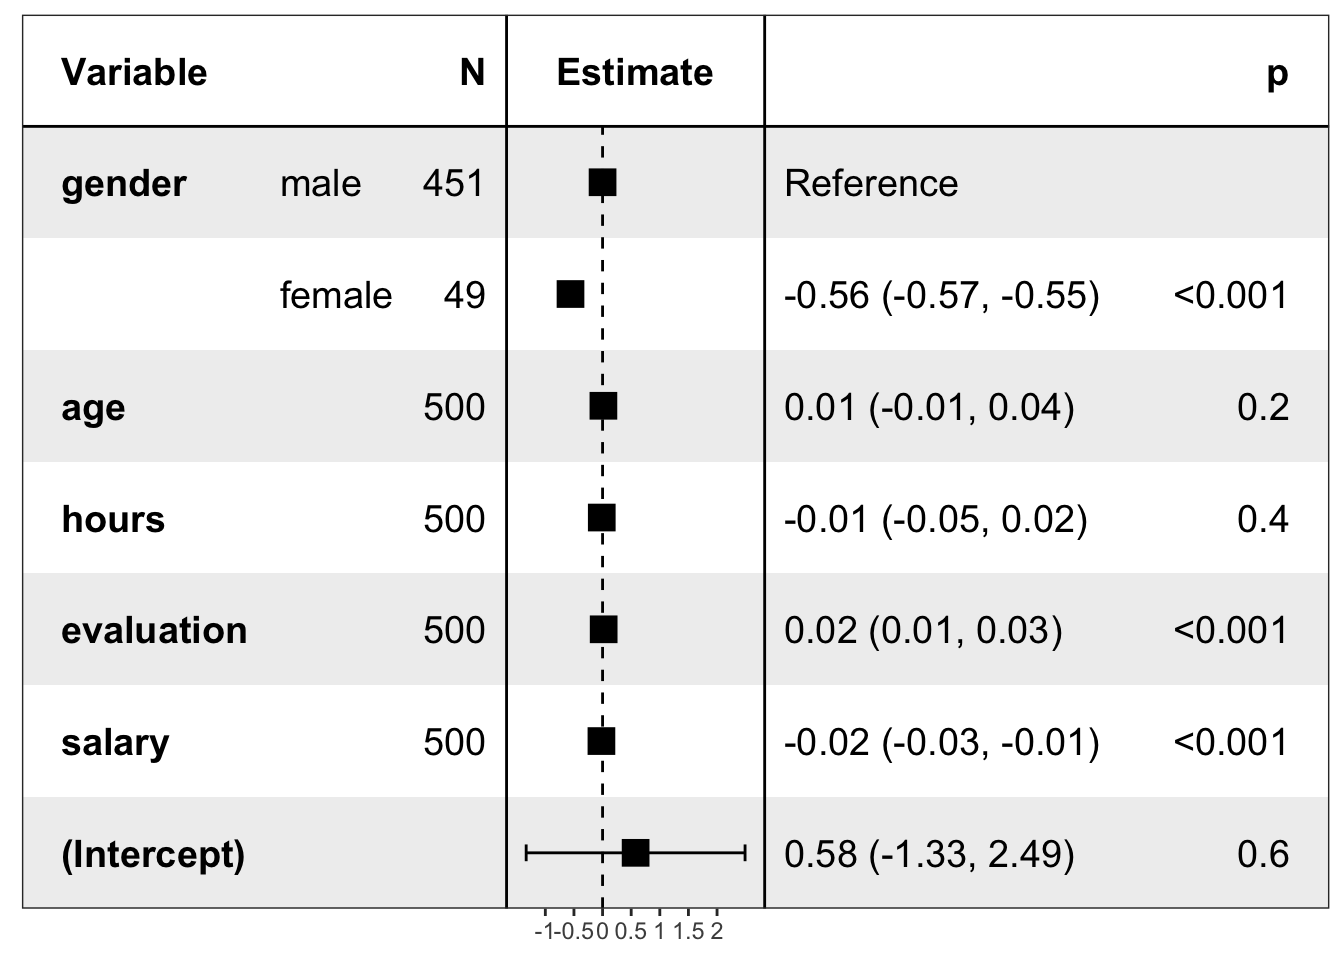
\includegraphics{PM_VEE_files/figure-latex/unnamed-chunk-25-2.pdf}

\hypertarget{the-iml-package}{%
\subsubsection{\texorpdfstring{\textbf{The iml
package}}{The iml package}}\label{the-iml-package}}

\begin{Shaded}
\begin{Highlighting}[]
\KeywordTok{library}\NormalTok{(}\StringTok{"iml"}\NormalTok{)}

\NormalTok{explainer_rf =}\StringTok{ }\NormalTok{Predictor}\OperatorTok{$}\KeywordTok{new}\NormalTok{(rf_model, }\DataTypeTok{data =}\NormalTok{ HR[,}\DecValTok{1}\OperatorTok{:}\DecValTok{5}\NormalTok{])}
\NormalTok{white_box =}\StringTok{ }\NormalTok{LocalModel}\OperatorTok{$}\KeywordTok{new}\NormalTok{(explainer_rf, }\DataTypeTok{x.interest =}\NormalTok{ new_observation[,}\DecValTok{1}\OperatorTok{:}\DecValTok{5}\NormalTok{], }\DataTypeTok{k =} \DecValTok{5}\NormalTok{)}
\NormalTok{white_box}
\end{Highlighting}
\end{Shaded}

\begin{verbatim}
## Interpretation method:  LocalModel 
## 
## 
## Analysed predictor: 
## Prediction task: unknown 
## 
## 
## Analysed data:
## Sampling from data.frame with 7847 rows and 5 columns.
## 
## Head of results:
##           beta x.recoded      effect x.original     feature feature.value
## 1  0.076624963       1.0  0.07662496       male gender=male   gender=male
## 2  0.005645199      57.7  0.32572799       57.7         age      age=57.7
## 3 -0.090849865      42.3 -3.84294931       42.3       hours    hours=42.3
## 4 -0.508827527       2.0 -1.01765505          2  evaluation  evaluation=2
## 5 -0.032375966       2.0 -0.06475193          2      salary      salary=2
## 6 -0.024263756       1.0 -0.02426376       male gender=male   gender=male
##   .class
## 1  fired
## 2  fired
## 3  fired
## 4  fired
## 5  fired
## 6     ok
\end{verbatim}

\begin{Shaded}
\begin{Highlighting}[]
\KeywordTok{plot}\NormalTok{(white_box)}
\end{Highlighting}
\end{Shaded}

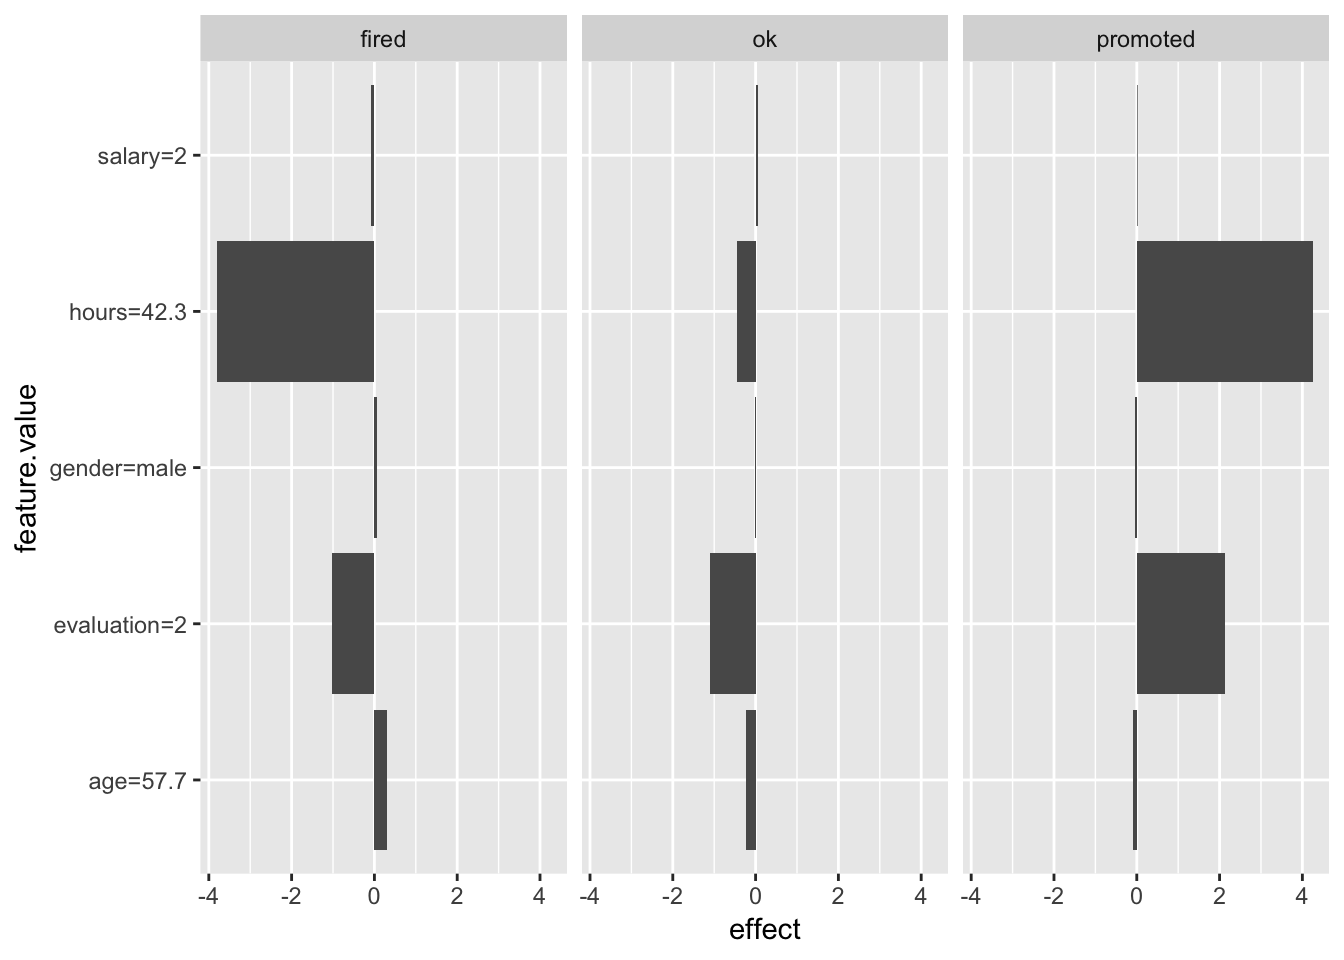
\includegraphics{PM_VEE_files/figure-latex/unnamed-chunk-26-1.pdf}

\hypertarget{ceterisParibus}{%
\section{What-If analysis with the Ceteris Paribus
Principle}\label{ceterisParibus}}

In this section we introduce tools based on Ceteris Paribus principle.
The main goal for these tools is to help understand how changes in model
input affect changes in model output.

Presented explainers are linked with the second law introduced in
Section \ref{three-single-laws}, i.e.~law for prediction's speculations.
This is why these explainers are also known as \emph{What-If model
analysis} or \emph{Individual Conditional EXpectations} \citep{ICEbox}.
It turns out that it is easier to understand how blacx-box model is
working if we can play with it by changing variable by variable.

\hypertarget{introduction-1}{%
\subsection{Introduction}\label{introduction-1}}

\emph{Ceteris paribus} is a Latin phrase meaning ``other things held
constant'' or ``all else unchanged''. Using this principle we examine
input variable per variable separatly, asumming that effects of all
other variables are unchanged. See Figure
\ref{fig:modelResponseCurveLine}

\begin{figure}

{\centering 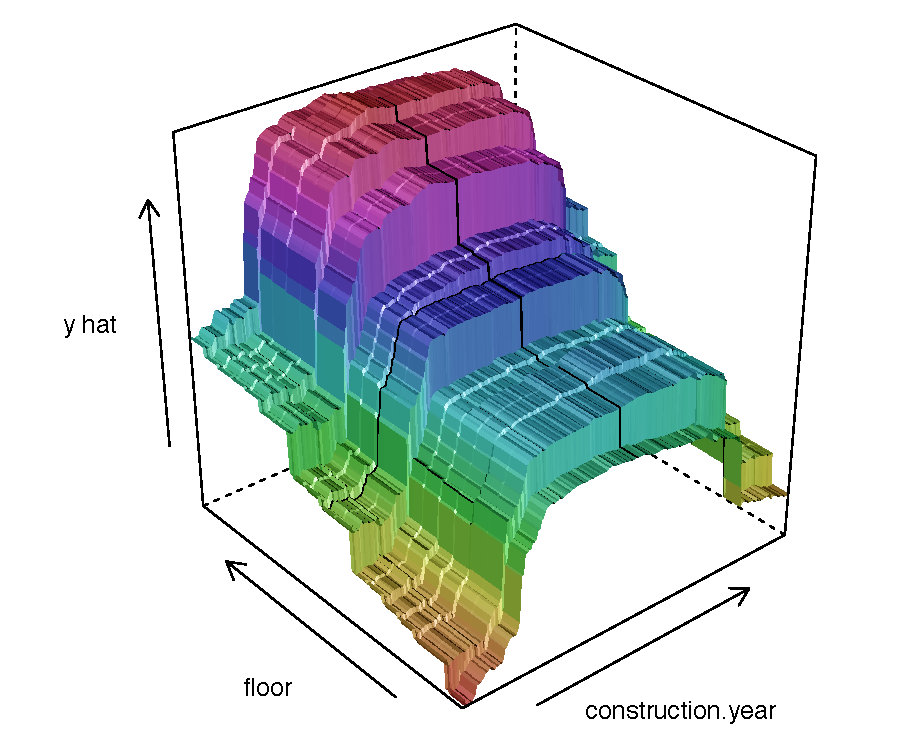
\includegraphics[width=0.7\linewidth]{figure/model_response_line} 

}

\caption{(fig:modelResponseCurveLine) A) Model response surface. Ceteris Paribus profiles marked with black curves helps to understand the curvature of the model response by updating only a single variable. B) CP profiles are individual conditional model responses}\label{fig:modelResponseCurveLine}
\end{figure}

Similar to the LIME method introduced in the section \ref{LIME}, Ceteris
Paribus profiles examine curvature of a model response function. The
difference between these two methods that LIME approximates the model
curvature with a simpler white-box model that is easier to present.
Usually the LIME model is sparse, thus our attention may be limited to
smaller number of dimensions. In contrary, the CP plots show conditional
model response for every variable. In the last subsection we discuss
pros and cons of this approach.

\hypertarget{intuition-5}{%
\subsection{Intuition}\label{intuition-5}}

\hypertarget{method-5}{%
\subsection{Method}\label{method-5}}

\hypertarget{ceterisParibus1d}{%
\subsubsection{1D profiles}\label{ceterisParibus1d}}

Let \(f_{M}(x): \mathcal R^{d} \rightarrow \mathcal R\) denote a
predictive model, i.e.~function that takes \(d\) dimensional vector and
calculate numerical score. Symbol \(x \in \mathcal R^d\) refers to a
point in the feature space. We use subscript \(x_i\) to refer to a
different data points and superscript \(x^j\) to refer to specific
dimensions. Additionally, let \(x^{-j}\) denote all coordinates except
\(j\)-th and let \(x|^j=z\) denote a data point \(x^*\) with all
coordinates equal to \(x\) except coordinate \(j\) equal to value \(z\).
I.e. \(\forall_{i \neq {j}} x^i = x^{*,i}\) and \(x^j = z\). In other
words \(x|^j=z\) denote a \(x\) with \(j\)th coordinate changed to
\(z\).

Now we can define uni-dimensional Ceteris Paribus Profile for model
\(f\), variable \(j\) and point \(x\) as

\[
CP^{f, j, x}(z) := f(x|^j = z).
\] I.e. CP profile is a model response obtained for observations created
based on \(x\) with coordinate \(j\) changed and all other coordinates
kept unchanged.

A natural way to visualise CP profiles is to use a profile plot as in
Figure \ref{fig:HRCPFiredHours}.

Figure \ref{fig:HRCPFiredHours} shows an example of Ceteris Paribus
profile. The black dot stands for prediction for a single observation.
Grey line show how the model response would change if in this single
observation coordinate \texttt{hours} will be changed to selected value.
One thing that we can read is that the model response is not smooth and
there is some variability along the profile. Second thing is that for
this particular observation the model response would drop significantly
if the variable \texttt{hours} will be higher than 45.

\begin{figure}

{\centering 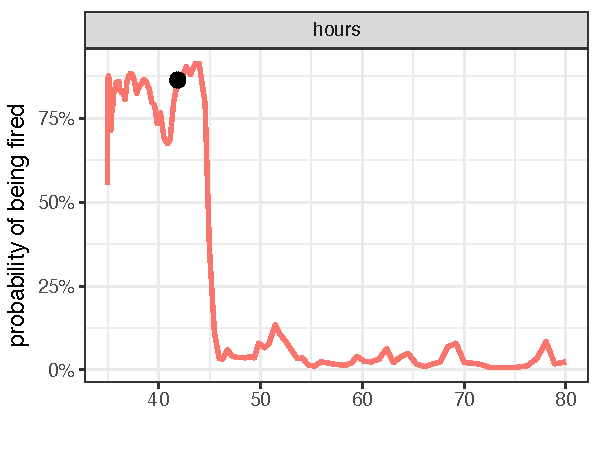
\includegraphics[width=0.5\linewidth]{figure/HR_cp_fired_hours} 

}

\caption{(fig:HRCPHiredHours) Ceteris Paribus profile for Random Forest model that assess the probability of being fired in call center as a function of average number of working hours}\label{fig:HRCPFiredHours}
\end{figure}

Since in the example dataset we are struggling with model for three
classes, one can plot CP profiles for each class in the same panel. See
an example in the Figure \ref{fig:HRCPAllHours}.

\begin{figure}

{\centering 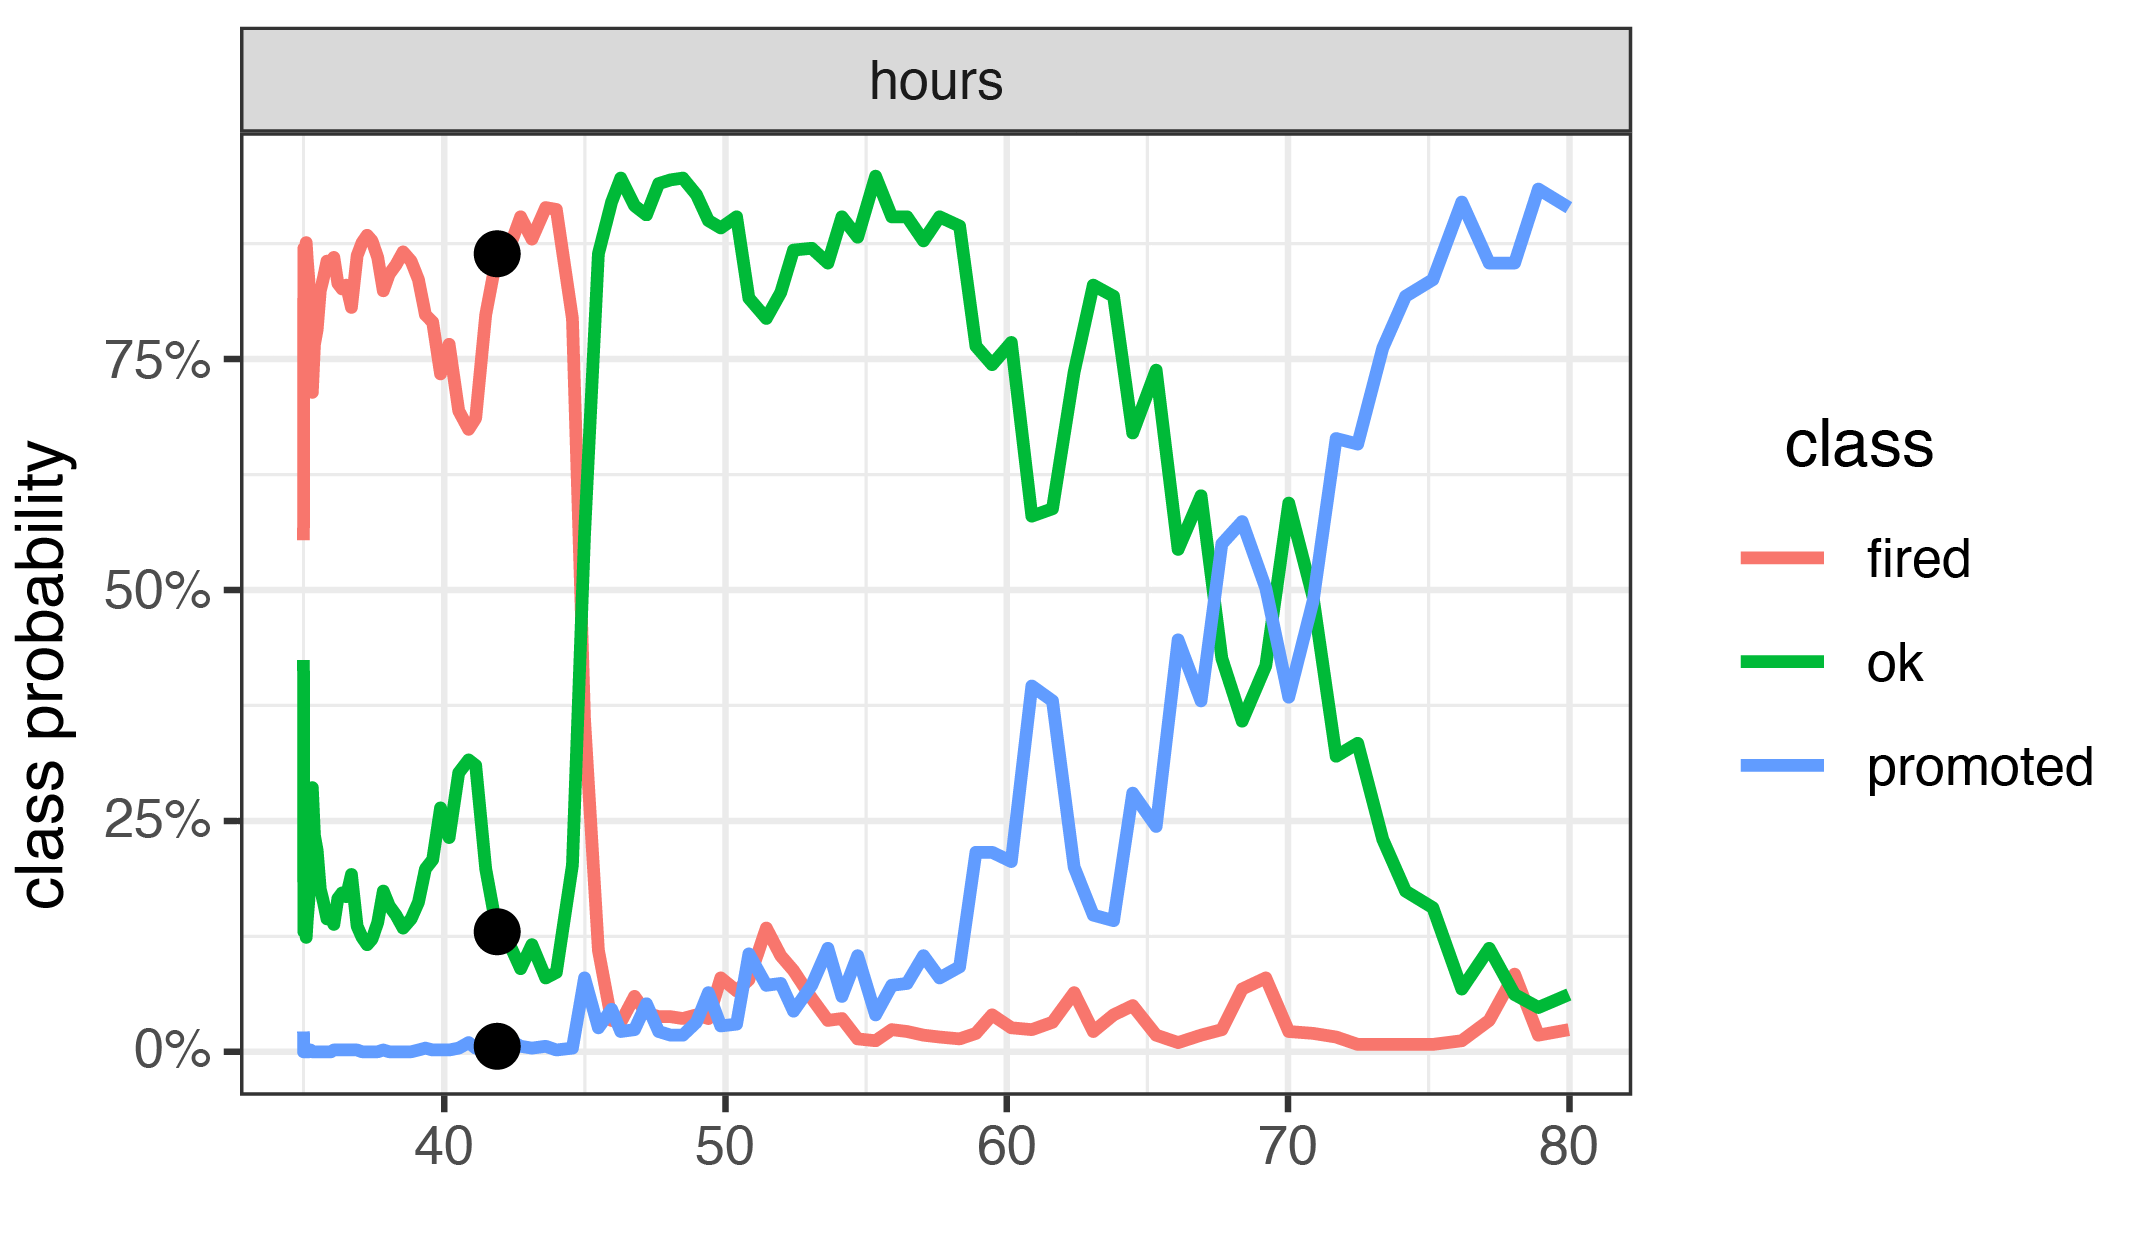
\includegraphics[width=0.6\linewidth]{figure/HR_cp_all_hours} 

}

\caption{(fig:HRCPAllHours) Ceteris Paribus profiles for three classess predicted by the Random Forest model as a function of average number of working hours}\label{fig:HRCPAllHours}
\end{figure}

Usually model input consist many variables, then it is beneficial to
show more variables at the same time. The easiest way to do so is to
plot consecutive variables on separate panels. See an example in Figure
\ref{fig:HRCPFiredAll}.

\begin{figure}

{\centering 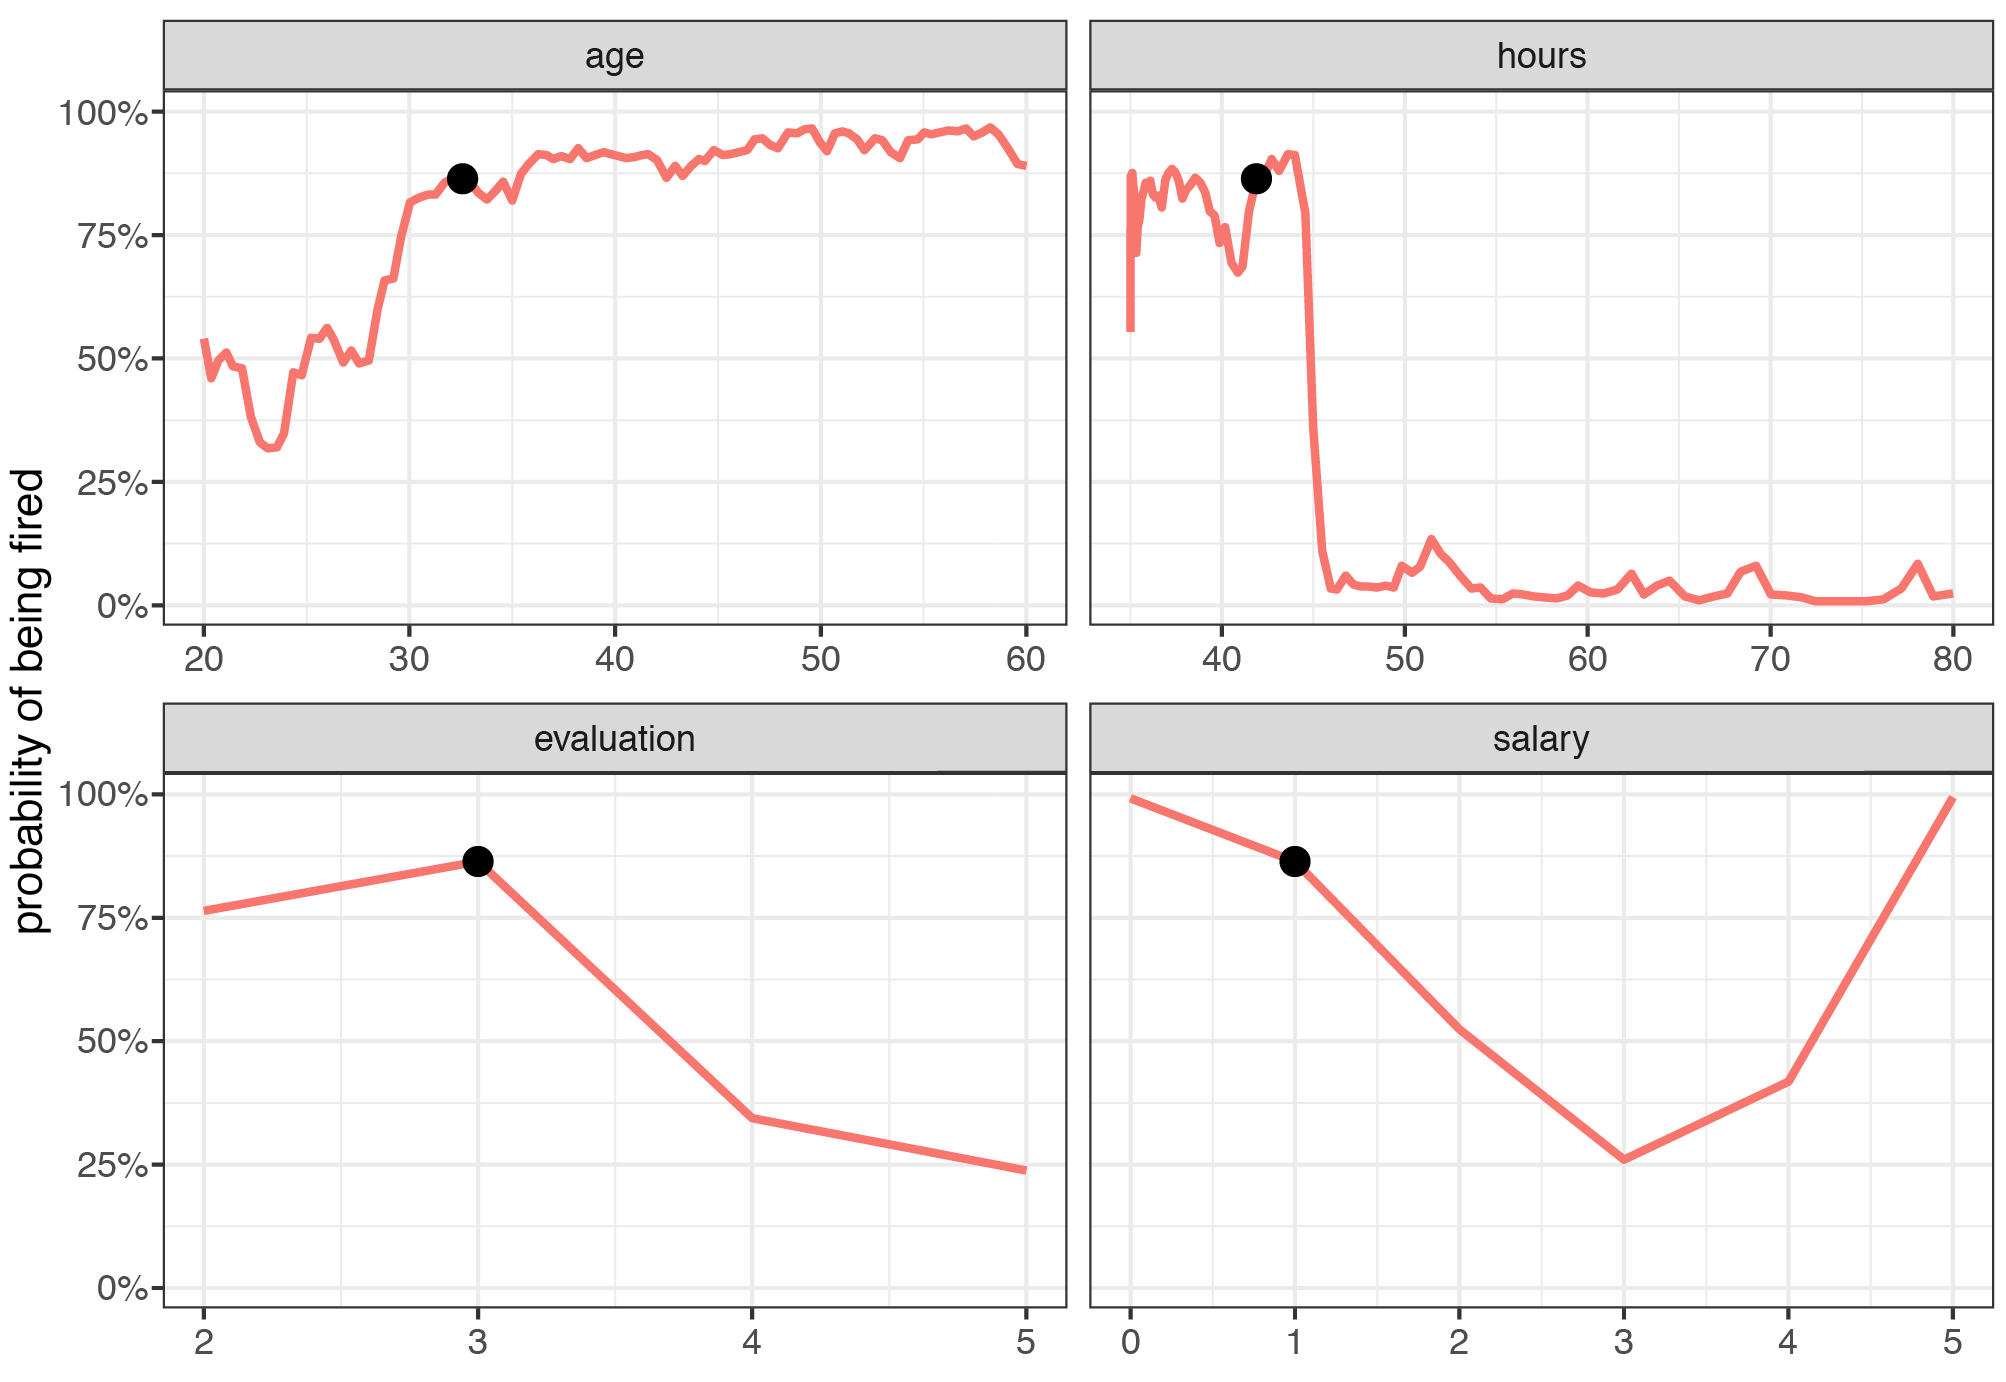
\includegraphics[width=0.7\linewidth]{figure/HR_cp_fired_all} 

}

\caption{(fig:HRCPFiredAll) Ceteris Paribus profiles for all continuous variables}\label{fig:HRCPFiredAll}
\end{figure}

\hypertarget{oscillations}{%
\subsubsection{Profile oscillations}\label{oscillations}}

Visual examination of variables is insightful, but for large number of
variables we end up with large number of panels, most of which are flat.
This is why we want to asses variable importance and show only profiles
for important variables. The advantage of CP profiles is that they lead
to a very natural and intuitive way of assessing the variable importance
for a single prediction. The intuition is: the more important variable
the larger are changes along the CP profile. If variable is not
important then model response will barely change. If variable is
important the CP profile change a lot for different values of a
variable.

Let's write it down in a more formal way.

Let \(vip^{CP}_j(x)\) denotes variable importance calculated based on CP
profiles in point \(x\) for variable \(j\).

\[
vip^{CP}_j(x) = \int_{-\inf}^{inf} |CP^{f,j,x}(z) - f(x)| dz
\]

So it's an absolute deviation from \(f(x)\). Note that one can consider
different modification of this coefficient:

\begin{enumerate}
\def\labelenumi{\arabic{enumi}.}
\tightlist
\item
  Deviations can be calculated not as a distance from \(f(x)\) but from
  average \(\bar CP^{f,j,x}(z)\).
\item
  The integral may be weighted based on the density of variable \(x^j\).
\item
  Instead of absolute deviations one may use root from average squares.
\end{enumerate}

TODO: we need to verify which approach is better. Anna Kozak is working
on this

The straightforward estimator for \(vip^{CP}_j(x)\) is

\[
\widehat{ vip^{CP}_j(x)} = \frac 1n \sum_{i=1}^n |CP^{f,j,x}(x_i) - f(x)|.
\]

Figure \ref{fig:CPVIPprofiles} shows the idea behind measuring
oscillations. The larger the highlighted area the more important is the
variable.

\begin{figure}

{\centering 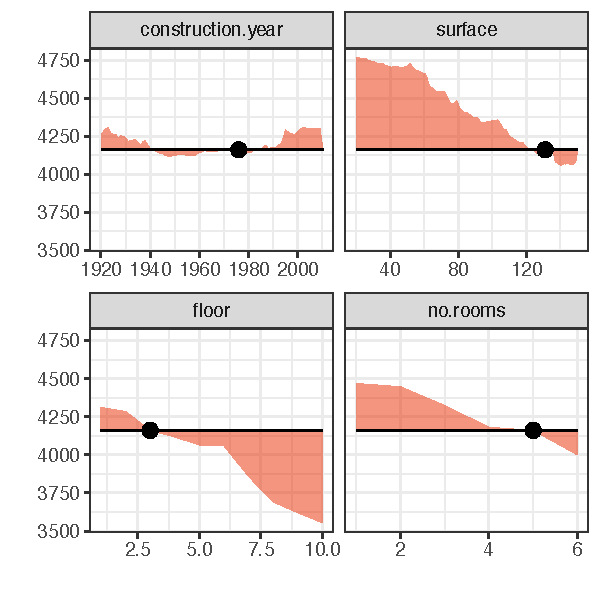
\includegraphics[width=0.5\linewidth]{figure/CP_VIP_profiles} 

}

\caption{(fig:CPVIPprofiles) CP oscillations are average deviations between CP profiles and the model response}\label{fig:CPVIPprofiles}
\end{figure}

Figure \ref{fig:CPVIP1} summarizes variable oscillations. Such visuals
help to quickly grasp how large are model oscillations around a specific
point.

\begin{figure}

{\centering 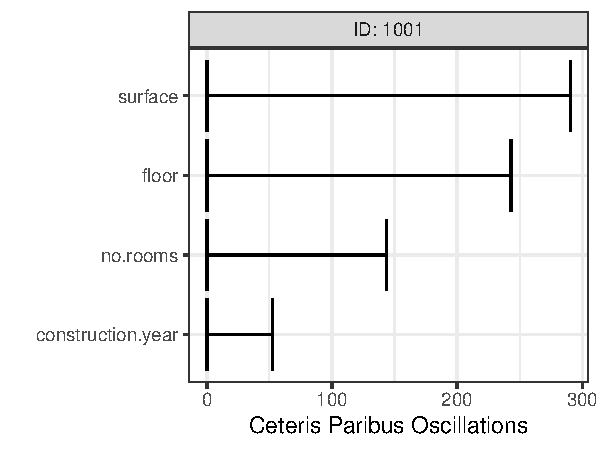
\includegraphics[width=0.4\linewidth]{figure/cp_vip_1} 

}

\caption{(fig:CPVIP1) Variable importance plots calculated for Ceteris Paribus profiles for observation ID: 1001}\label{fig:CPVIP1}
\end{figure}

\textbf{NOTE}

Variable importance for single prediction may be very different than
variable importance for the full model.

For example, consider a model \[
f(x_1, x_2) = x_1 * x_2
\] where variables \(x_1\) and \(x_2\) takes values in \([0,1]\).

From the global perspective both variables are equally important.

But local variable importance is very different. Around point
\(x = (0, 1)\) the importance of \(x_1\) is much larger than \(x_2\).
This is because profile for \(f(z, 1)\) have larger oscillations than
\(f(0, z)\).

\hypertarget{d-profiles}{%
\subsubsection{2D profiles}\label{d-profiles}}

The definition of ceteris paribus profiles given in section
\ref{ceterisParibus1d} may be easily extended to two and more variables.
Also definition of CP oscillations \ref{oscillations} have straight
forward generalization for larger number of dimensions. Such
generalisations are usefull when model is non additive. Presence of
pairwise interactions may be detected with 2D Ceteris Paribus plots.

Let's define two-dimensional Ceteris Paribus Profile for model \(f\),
variables \(j\) and \(k\) and point \(x\) as

\[
CP^{f, (j,k), x}(z_1, z_2) := f(x|^{(j,k)} = (z_1,z_2)).
\] I.e. CP profile is a model response obtained for observations created
based on \(x\) with \(j\) and \(k\) coordinates changed to
\((z_1, z_2)\) and all other coordinates kept unchanged.

A natural way to visualise 2D CP profiles is to use a level plot as in
Figure \ref{fig:CP2Dsurflor}.

\begin{figure}

{\centering 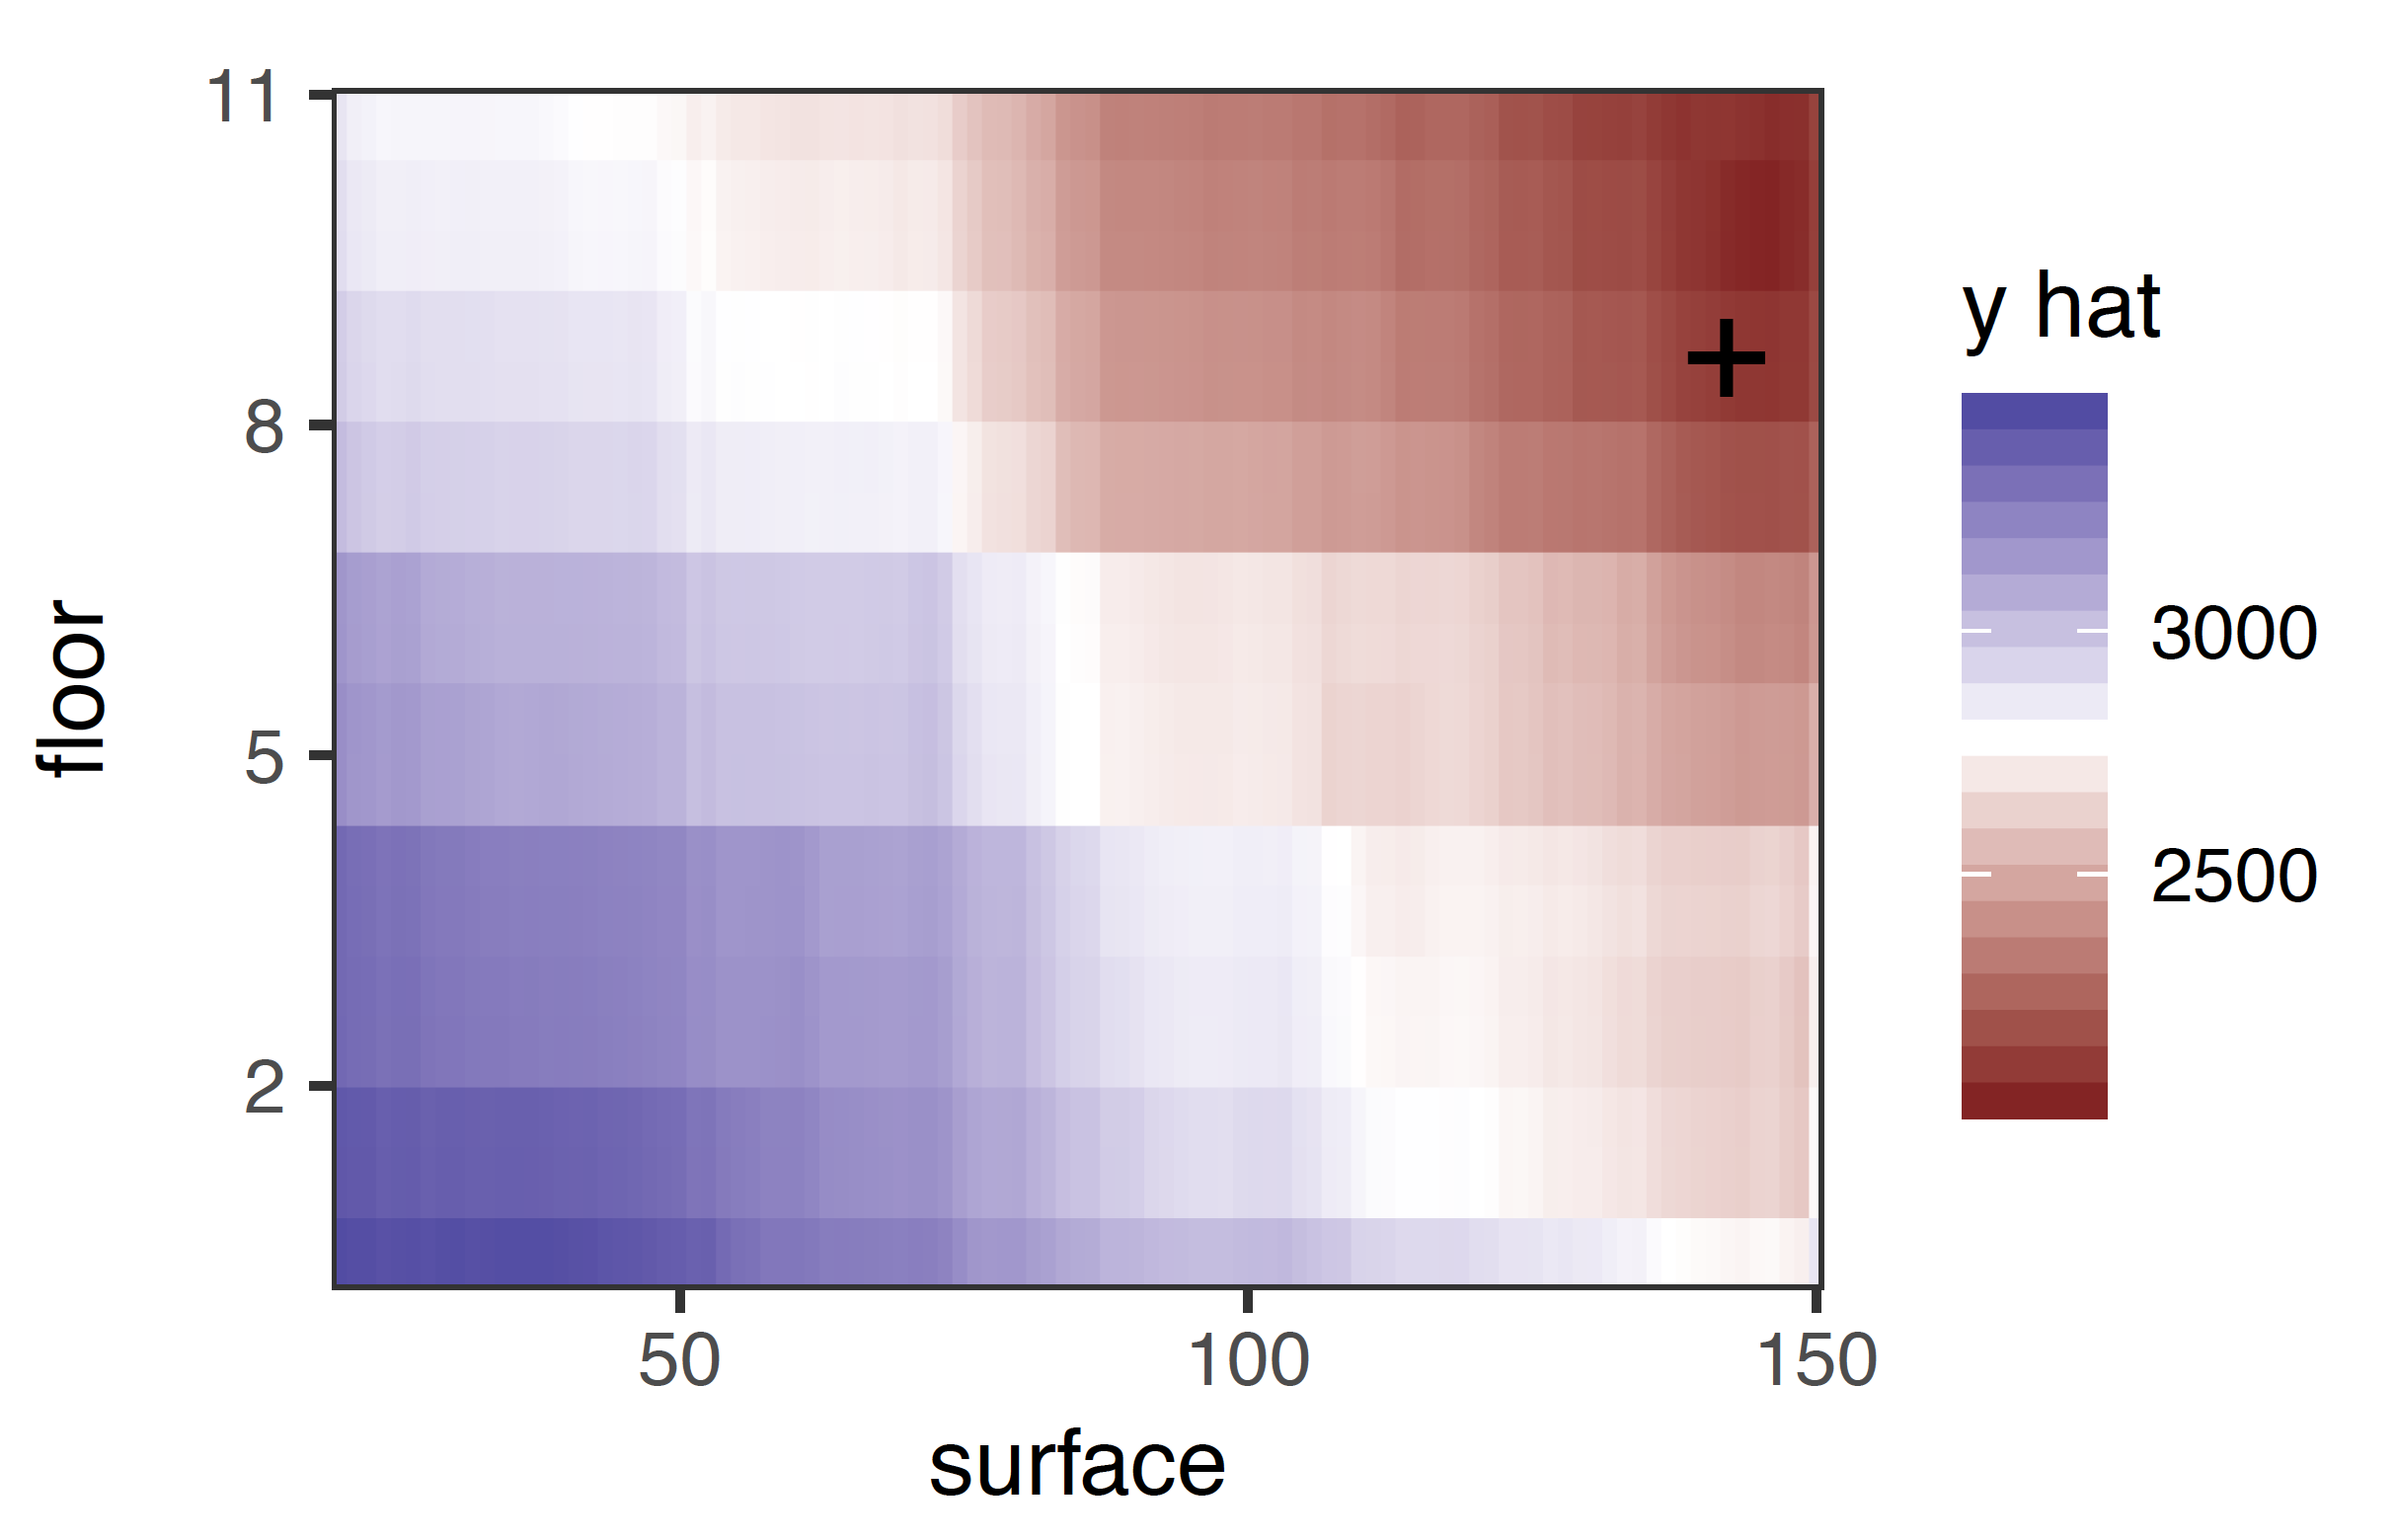
\includegraphics[width=0.6\linewidth]{figure/cp_2d_surf_floor} 

}

\caption{(fig:CP2Dsurflor) Ceteris Paribus plot for a pair of variales. Black cross marks coordinated for the observation of interest. Presented model estimates price of an appartment}\label{fig:CP2Dsurflor}
\end{figure}

If number of variables is small or moderate thein it is possible to
present all pairs of variables. See an example in Figure
\ref{fig:CP2Dall}.

\begin{figure}

{\centering 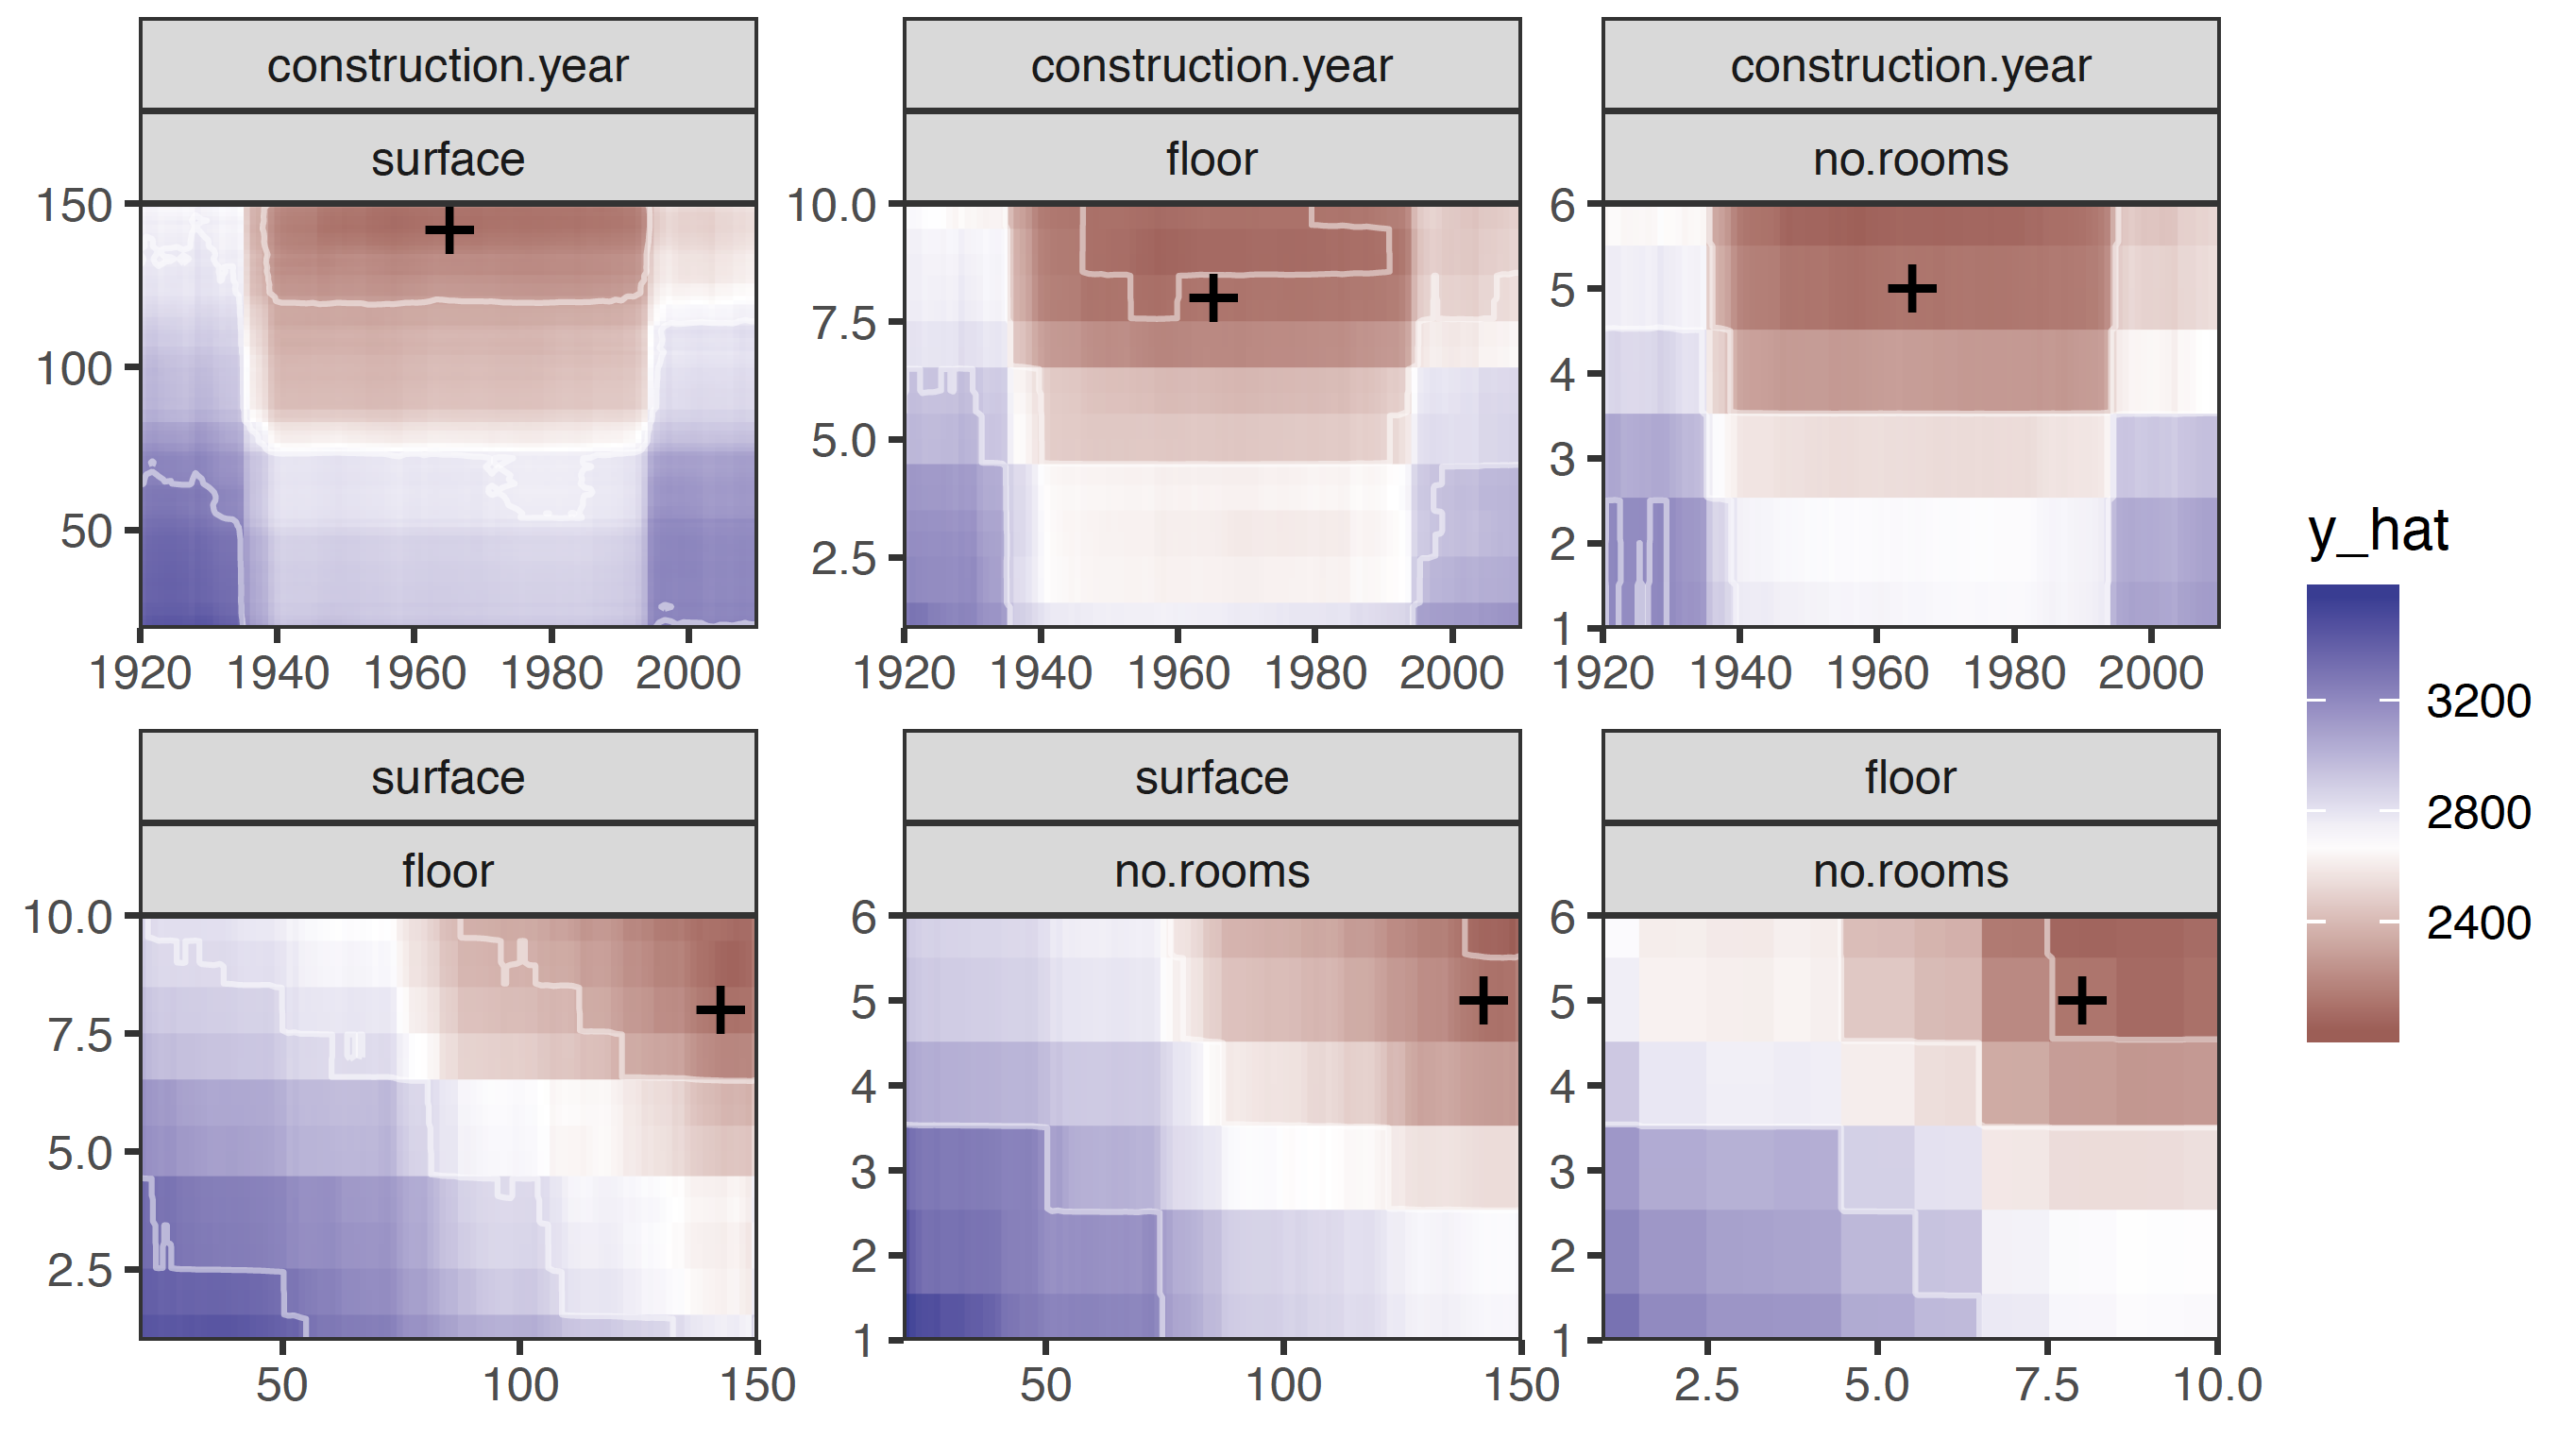
\includegraphics[width=0.9\linewidth]{figure/cp_2d_all} 

}

\caption{(fig:CP2Dall) Ceteris Paribus plot for all pairs of variales.}\label{fig:CP2Dall}
\end{figure}

\hypertarget{local-model-fidelity}{%
\subsection{Local model fidelity}\label{local-model-fidelity}}

Ceteris Paribus profiles are also a useful tool to validate local model
fidelity. It may happen that global performance of the model is good,
while for some points the local fit is very bad. Local fidelity helps to
understand how good is the model fit around point of interest.

How does it work?

The idea behind fidelity plots is to select some number of points from
the validation dataset that are closes to the point of interest. It's a
similar approach as in k nearest neighbours. Then for these neighbours
we may plot Ceteris Paribus Profiles and check how stable they are.

Also, if we know true taget values for points from the validation
dataset we may plot residuals to show how large are residuals.

An example fidelity plot is presented in Figure \ref{fig:CPfidelity1}.
Black line shows the CP profiles for the point of interest, while grey
lines show CP profiles for neihgbors. Red intervals stand for residuals
and in this example it looks like residuals for neighbours are all
negative. Thus maybe model is biased around the point of interest.

\begin{figure}

{\centering 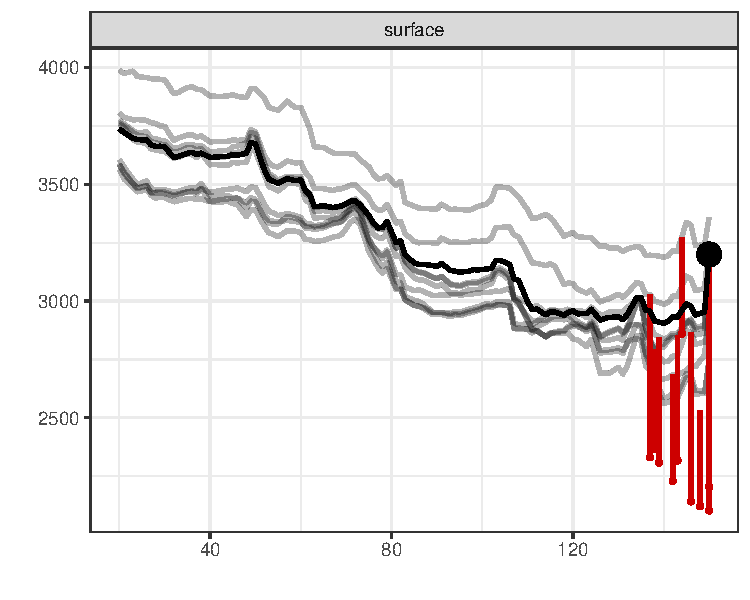
\includegraphics[width=0.7\linewidth]{figure/cp_fidelity_1} 

}

\caption{(fig:CPfidelity1) Local fidelity plots. Black line shows the CP profile for the point of interest. Grey lines show CP profiles for nearest neighbors. Red intervals correspond to residuals. Each red interval starts in a model prediction for a selected neighbor and ends in its true value of target variable.}\label{fig:CPfidelity1}
\end{figure}

This observation may be confirmed by plots that compare distribution of
all residuals against distribution of residuals for neighbors.

See Figure \ref{CPfidelityBoxplot} for an example. Here residuals for
neighbors are shifted towards highest values. This suggests that the
model response is biased around the observation of interest.

\begin{figure}

{\centering 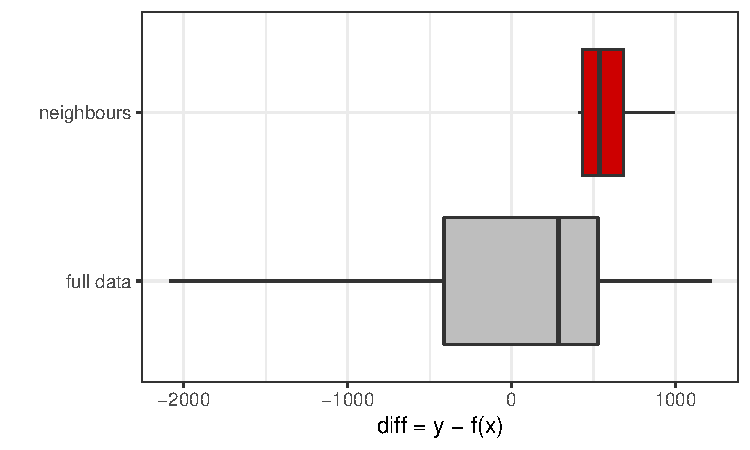
\includegraphics[width=0.7\linewidth]{figure/cp_fidelity_boxplot} 

}

\caption{(fig:CPfidelityBoxplot) Distribution of residuals for whole validation data (grey boxplot) and for selected closes 15 neighbors (red boxplot).}\label{fig:CPfidelityBoxplot}
\end{figure}

\hypertarget{example}{%
\subsection{Example}\label{example}}

\hypertarget{pros-and-cons-5}{%
\subsection{Pros and cons}\label{pros-and-cons-5}}

Ceteris Paribus principle gives a uniform and extendable approach to
model exploration. Below we summarize key strengths and weaknesses of
this approach.

\textbf{Pros}

\begin{itemize}
\tightlist
\item
  Graphical representation of Ceteris Paribus profile is easy to
  understand.
\item
  Ceteris Paribus profiles are compact and it is easy to fit many models
  or many variables in a small space.
\item
  Ceteris Paribus profiles helps to understand how model response would
  change and how stable it is
\item
  Oscillations calculated for CP profiles helps to select the most
  important variables.
\item
  2D Ceteris Paribus profiles help to identify pairwise interactions
  between variables.
\end{itemize}

\textbf{Cons}

\begin{itemize}
\tightlist
\item
  If variables are correlated (like surface and number of rooms) then
  the `\emph{everything else kept unchanged}' approach leads to
  unrealistic settings.
\item
  Interactions between variables are not visible in 1D plots.
\item
  This tool is not suited for very wide data, like hundreds or thousands
  of variables.
\item
  Visualization of categorical variables is non trivial.
\end{itemize}

\hypertarget{code-snippets-for-r-4}{%
\subsection{Code snippets for R}\label{code-snippets-for-r-4}}

In this section we present key features of the \texttt{ceterisParibus}
package for R \citep{R-ceterisParibus}. This package covers all features
presented in this chapter. It is available on CRAN and GitHub. Find more
examples at the website of this package
\texttt{https://pbiecek.github.io/ceterisParibus/}.

A very interesting tool for moedl explorartion with similar principle is
implemented in the \texttt{condvis} package \citep{JSSv081i05}.

\textbf{Model preparation}

In this section we will present examples based on the
\texttt{apartments} dataset. See section TODO for more details.

\begin{Shaded}
\begin{Highlighting}[]
\KeywordTok{library}\NormalTok{(}\StringTok{"DALEX"}\NormalTok{)}
\KeywordTok{head}\NormalTok{(apartments)}
\end{Highlighting}
\end{Shaded}

\begin{verbatim}
##   m2.price construction.year surface floor no.rooms    district
## 1     5897              1953      25     3        1 Srodmiescie
## 2     1818              1992     143     9        5     Bielany
## 3     3643              1937      56     1        2       Praga
## 4     3517              1995      93     7        3      Ochota
## 5     3013              1992     144     6        5     Mokotow
## 6     5795              1926      61     6        2 Srodmiescie
\end{verbatim}

The problem here is to predict average price for square meter for an
apartment. Let's build a random forest model with \texttt{randomForest}
package \citep{R-randomForest}.

\begin{Shaded}
\begin{Highlighting}[]
\KeywordTok{library}\NormalTok{(}\StringTok{"randomForest"}\NormalTok{)}
\NormalTok{rf_model <-}\StringTok{ }\KeywordTok{randomForest}\NormalTok{(m2.price }\OperatorTok{~}\StringTok{ }\NormalTok{construction.year }\OperatorTok{+}\StringTok{ }\NormalTok{surface }\OperatorTok{+}\StringTok{ }\NormalTok{floor }\OperatorTok{+}
\StringTok{      }\NormalTok{no.rooms, }\DataTypeTok{data =}\NormalTok{ apartments)}
\NormalTok{rf_model}
\end{Highlighting}
\end{Shaded}

\begin{verbatim}
## 
## Call:
##  randomForest(formula = m2.price ~ construction.year + surface +      floor + no.rooms, data = apartments) 
##                Type of random forest: regression
##                      Number of trees: 500
## No. of variables tried at each split: 1
## 
##           Mean of squared residuals: 487092.2
##                     % Var explained: 40.69
\end{verbatim}

Model exploration with \texttt{ceterisParibus} package is performed in
four steps.

\textbf{1. Create an explainer - wrapper around model and validation
data.}

Since all other functions work in a model agnostic fashion, first we
need to define a wrapper around the model. Here we are using the
\texttt{explain()} function from \texttt{DALEX} package \citep{R-DALEX}.

\begin{Shaded}
\begin{Highlighting}[]
\KeywordTok{library}\NormalTok{(}\StringTok{"DALEX"}\NormalTok{)}
\NormalTok{explainer_rf <-}\StringTok{ }\KeywordTok{explain}\NormalTok{(rf_model,}
      \DataTypeTok{data =}\NormalTok{ apartmentsTest, }\DataTypeTok{y =}\NormalTok{ apartmentsTest}\OperatorTok{$}\NormalTok{m2.price)}
\NormalTok{explainer_rf}
\end{Highlighting}
\end{Shaded}

\begin{verbatim}
## Model label:  randomForest 
## Model class:  randomForest.formula,randomForest 
## Data head  :
##      m2.price construction.year surface floor no.rooms    district
## 1001     4644              1976     131     3        5 Srodmiescie
## 1002     3082              1978     112     9        4     Mokotow
\end{verbatim}

\textbf{2. Define point of interest.}

Certeris Paribus profiles explore model around a single point.

\begin{Shaded}
\begin{Highlighting}[]
\NormalTok{new_apartment <-}\StringTok{ }\KeywordTok{data.frame}\NormalTok{(}\DataTypeTok{construction.year =} \DecValTok{1965}\NormalTok{, }\DataTypeTok{no.rooms =} \DecValTok{5}\NormalTok{, }\DataTypeTok{surface =} \DecValTok{142}\NormalTok{, }\DataTypeTok{floor =} \DecValTok{8}\NormalTok{)}
\NormalTok{new_apartment}
\end{Highlighting}
\end{Shaded}

\begin{verbatim}
##   construction.year no.rooms surface floor
## 1              1965        5     142     8
\end{verbatim}

\begin{Shaded}
\begin{Highlighting}[]
\KeywordTok{predict}\NormalTok{(rf_model, new_apartment)}
\end{Highlighting}
\end{Shaded}

\begin{verbatim}
##        1 
## 2327.341
\end{verbatim}

\textbf{3. Calculate CP profiles}

The \texttt{ceteris\_paribus()} function calculates CP profiles for
selected model around selected observation.

By default CP profiles are calculated for all numerical variables. Use
the \texttt{variables} argument to select subset of interesting
variables. The result from \texttt{ceteris\_paribus()}function is a data
frame with model predictions for modified points around the point of
interest.

\begin{Shaded}
\begin{Highlighting}[]
\KeywordTok{library}\NormalTok{(}\StringTok{"ceterisParibus"}\NormalTok{)}
\NormalTok{cp_rf <-}\StringTok{ }\KeywordTok{ceteris_paribus}\NormalTok{(explainer_rf, new_apartment, }
                            \DataTypeTok{variables =} \KeywordTok{c}\NormalTok{(}\StringTok{"construction.year"}\NormalTok{, }\StringTok{"floor"}\NormalTok{))}
\NormalTok{cp_rf}
\end{Highlighting}
\end{Shaded}

\begin{verbatim}
## Top profiles    : 
##     construction.year no.rooms surface floor   _yhat_           _vname_
## 1                1920        5     142     8 3074.184 construction.year
## 1.1              1921        5     142     8 3097.319 construction.year
## 1.2              1922        5     142     8 3085.503 construction.year
## 1.3              1923        5     142     8 3056.904 construction.year
## 1.4              1923        5     142     8 3056.904 construction.year
## 1.5              1924        5     142     8 3070.891 construction.year
##     _ids_      _label_
## 1       1 randomForest
## 1.1     1 randomForest
## 1.2     1 randomForest
## 1.3     1 randomForest
## 1.4     1 randomForest
## 1.5     1 randomForest
## 
## 
## Top observations:
##   construction.year no.rooms surface floor   _yhat_      _label_
## 1              1965        5     142     8 2327.341 randomForest
\end{verbatim}

\textbf{4. Plot CP profiles.}

Generic \texttt{plot()} function plot CP profiles. It returns a
\texttt{ggplot2} object that can be polished if needed. Use additional
arguments of this function to select colors and sizes for elements
visible in the plot.

\begin{Shaded}
\begin{Highlighting}[]
\KeywordTok{plot}\NormalTok{(cp_rf) }
\end{Highlighting}
\end{Shaded}

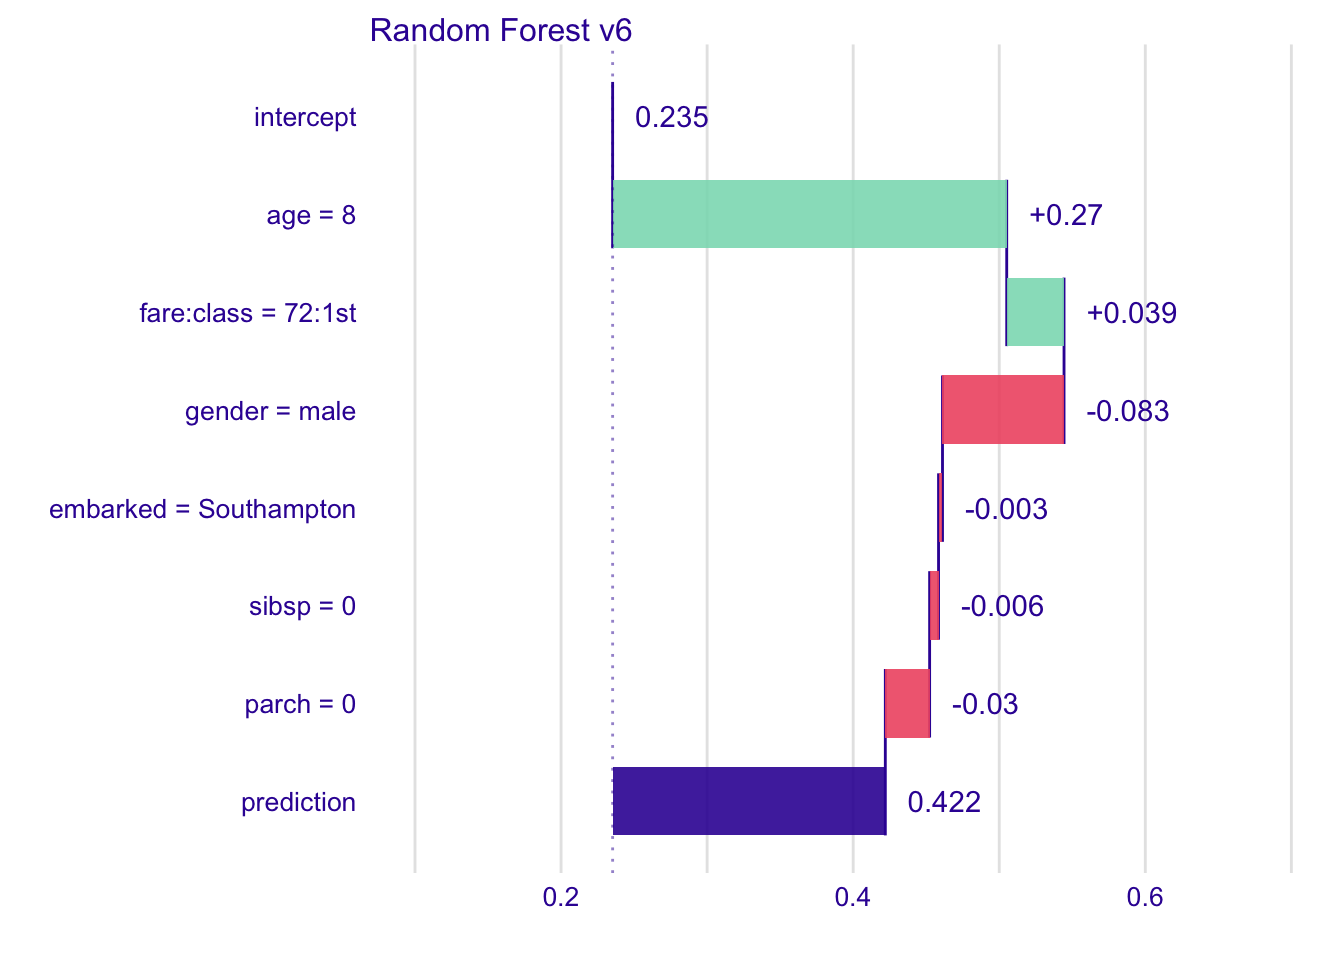
\includegraphics{PM_VEE_files/figure-latex/unnamed-chunk-32-1.pdf}

One of very useful features of \texttt{ceterisParibus} explainers is
that profiles for two or more models may be superimposed in a single
plot. This helps in model comparisons.

Let's create a linear model for this dataset and repeat steps 1-3 for
the lm model.

\begin{Shaded}
\begin{Highlighting}[]
\NormalTok{lm_model <-}\StringTok{ }\KeywordTok{lm}\NormalTok{(m2.price }\OperatorTok{~}\StringTok{ }\NormalTok{construction.year }\OperatorTok{+}\StringTok{ }\NormalTok{surface }\OperatorTok{+}\StringTok{ }\NormalTok{floor }\OperatorTok{+}
\StringTok{      }\NormalTok{no.rooms, }\DataTypeTok{data =}\NormalTok{ apartments)}
\NormalTok{explainer_lm <-}\StringTok{ }\KeywordTok{explain}\NormalTok{(lm_model,}
      \DataTypeTok{data =}\NormalTok{ apartmentsTest, }\DataTypeTok{y =}\NormalTok{ apartmentsTest}\OperatorTok{$}\NormalTok{m2.price)}
\NormalTok{cp_lm <-}\StringTok{ }\KeywordTok{ceteris_paribus}\NormalTok{(explainer_lm, new_apartment, }
                            \DataTypeTok{variables =} \KeywordTok{c}\NormalTok{(}\StringTok{"construction.year"}\NormalTok{, }\StringTok{"floor"}\NormalTok{))}
\end{Highlighting}
\end{Shaded}

Now we can use function \texttt{plot()} to compare both models in a
single chart. Additional argument \texttt{color\ =\ "\_label\_"} set
color as a key for model.

\begin{Shaded}
\begin{Highlighting}[]
\KeywordTok{plot}\NormalTok{(cp_rf, cp_lm, }\DataTypeTok{color =} \StringTok{"_label_"}\NormalTok{)}
\end{Highlighting}
\end{Shaded}

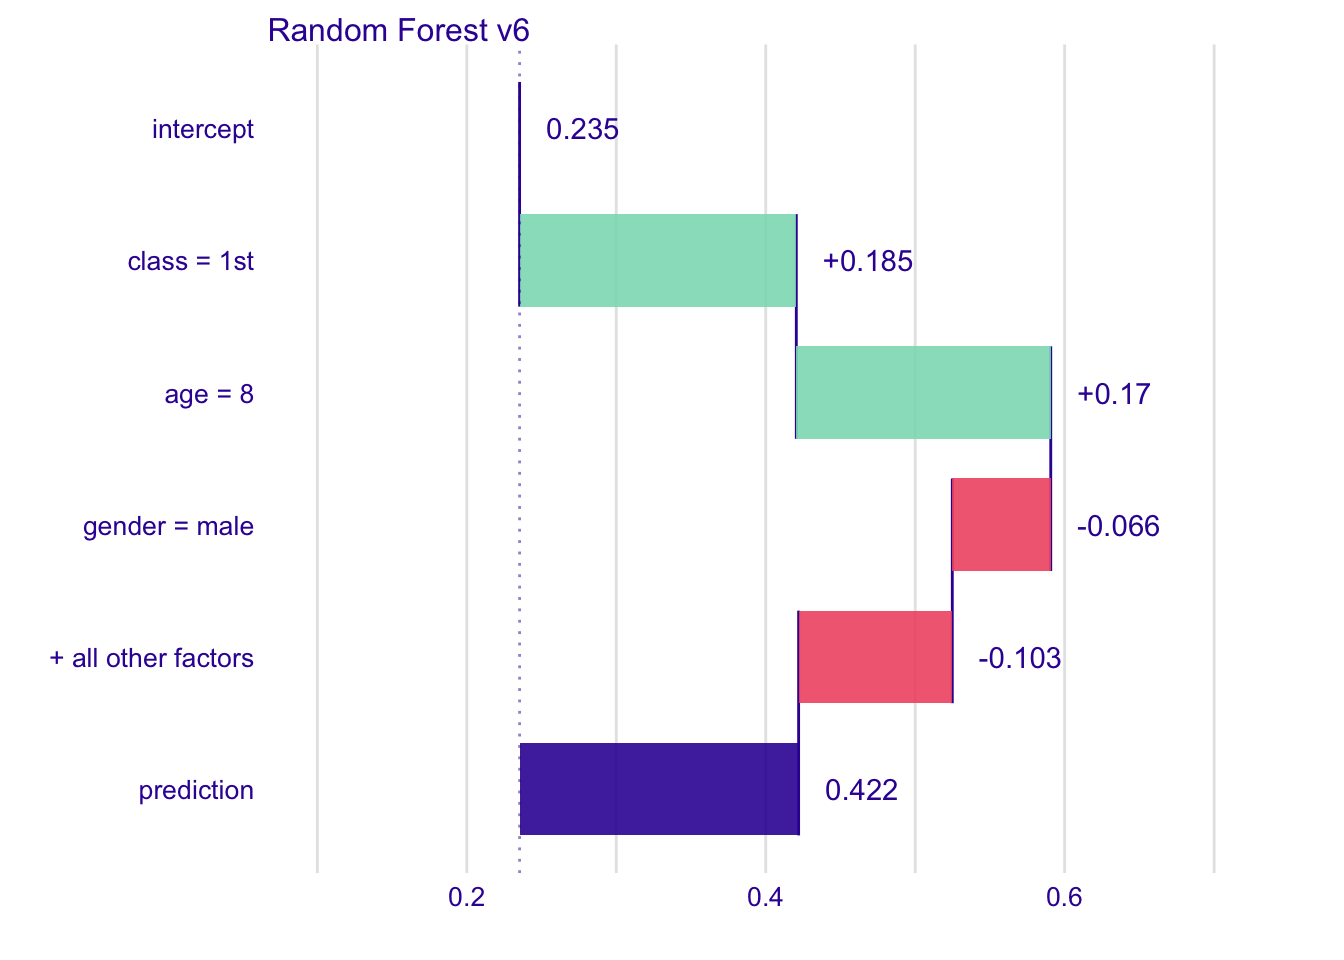
\includegraphics{PM_VEE_files/figure-latex/unnamed-chunk-34-1.pdf}

\textbf{Oscillations}

The \texttt{calculate\_oscillations()} function calculates oscillations
for CP profiles.

\begin{Shaded}
\begin{Highlighting}[]
\NormalTok{cp_rf_all <-}\StringTok{ }\KeywordTok{ceteris_paribus}\NormalTok{(explainer_rf, new_apartment)}
\NormalTok{co_rf_all <-}\StringTok{ }\KeywordTok{calculate_oscillations}\NormalTok{(cp_rf_all)}
\NormalTok{co_rf_all}
\end{Highlighting}
\end{Shaded}

\begin{verbatim}
##             _vname_ _ids_ oscillations
## 2           surface     1     647.6881
## 4          no.rooms     1     404.0211
## 3             floor     1     333.8213
## 1 construction.year     1     239.7179
\end{verbatim}

\begin{Shaded}
\begin{Highlighting}[]
\KeywordTok{plot}\NormalTok{(co_rf_all)}
\end{Highlighting}
\end{Shaded}

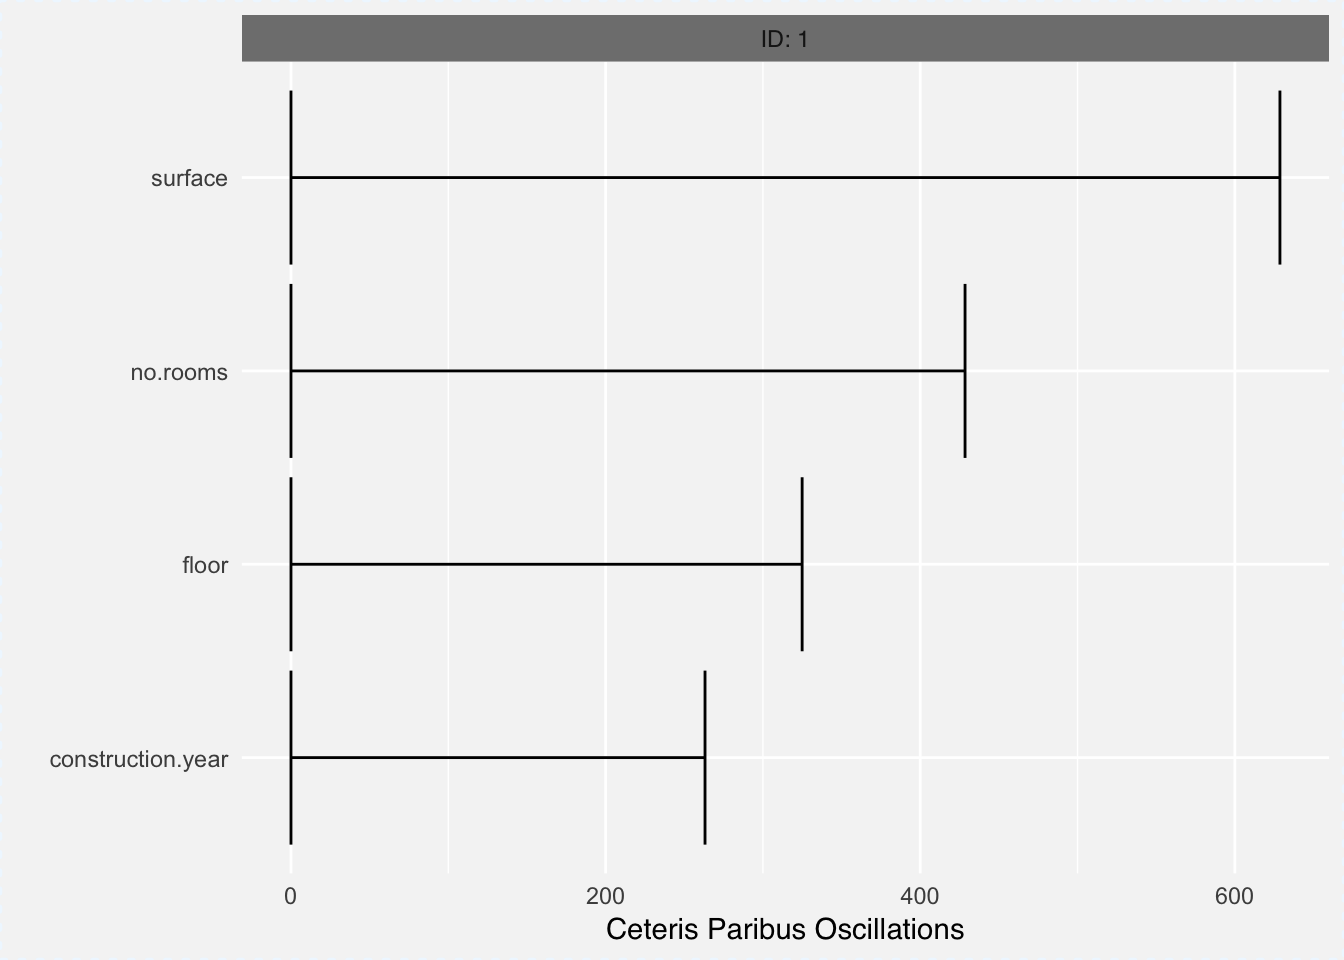
\includegraphics{PM_VEE_files/figure-latex/unnamed-chunk-35-1.pdf}

\textbf{2D Ceteris Paribus profiles}

And the \texttt{what\_if\_2d()} function calculates 2D CP profiles.

\begin{Shaded}
\begin{Highlighting}[]
\NormalTok{wi_rf_2d <-}\StringTok{ }\KeywordTok{what_if_2d}\NormalTok{(explainer_rf, }\DataTypeTok{observation =}\NormalTok{ new_apartment, }
                 \DataTypeTok{selected_variables =} \KeywordTok{c}\NormalTok{(}\StringTok{"surface"}\NormalTok{,}\StringTok{"floor"}\NormalTok{, }\StringTok{"construction.year"}\NormalTok{))}
\KeywordTok{plot}\NormalTok{(wi_rf_2d, }\DataTypeTok{split_ncol =} \DecValTok{2}\NormalTok{)}
\end{Highlighting}
\end{Shaded}

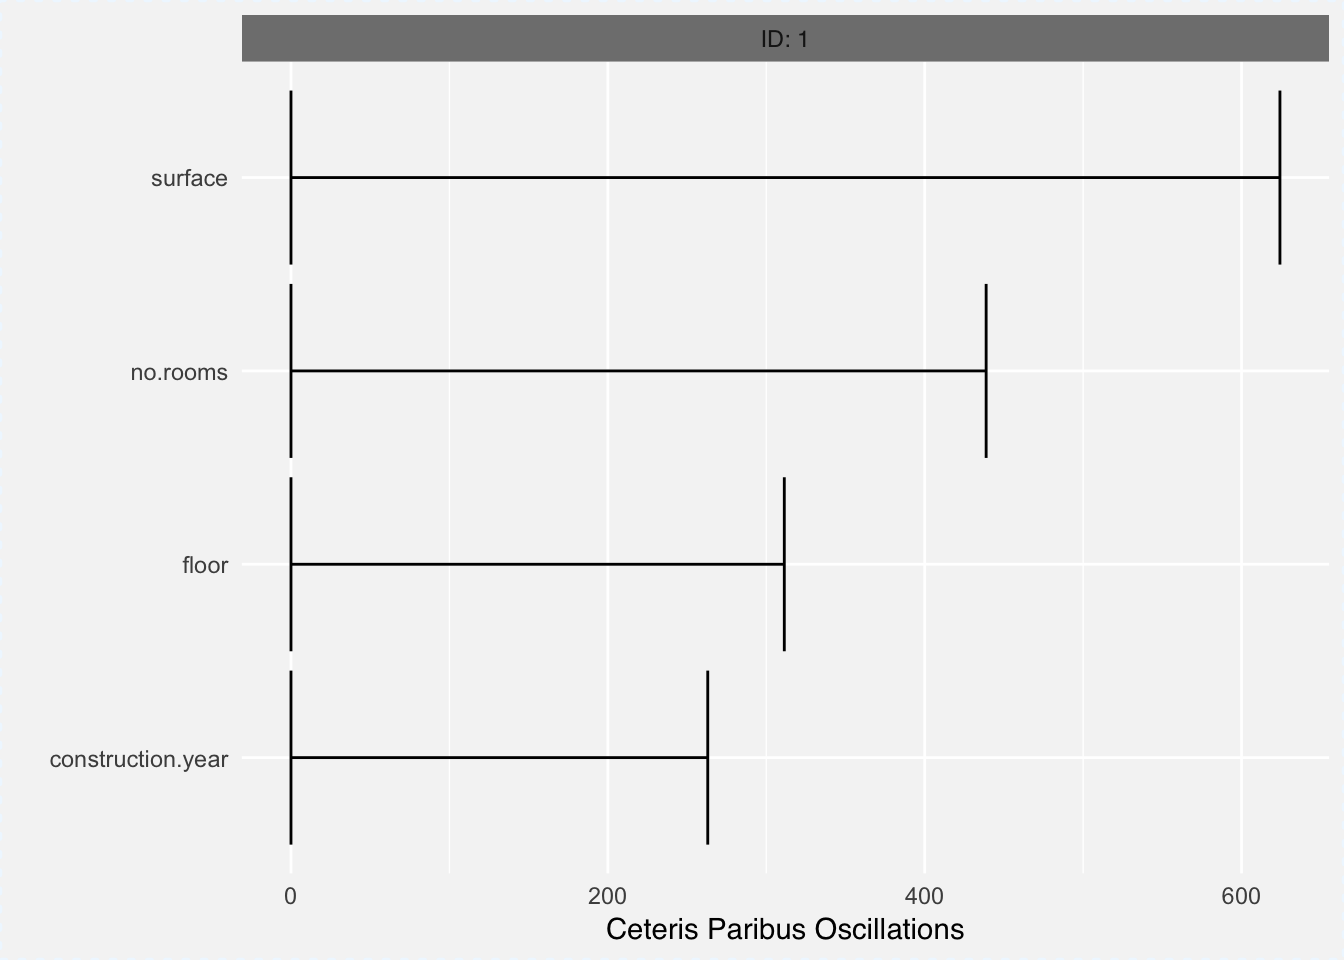
\includegraphics{PM_VEE_files/figure-latex/unnamed-chunk-36-1.pdf}

\hypertarget{comparision-of-prediction-level-explainers}{%
\section{Comparision of prediction level
explainers}\label{comparision-of-prediction-level-explainers}}

TODO

compare pros and cons of different techniques

\hypertarget{when-to-use}{%
\subsection{When to use?}\label{when-to-use}}

There are several use-cases for such explainers. Think about following.

\begin{itemize}
\tightlist
\item
  Model improvement. If model works particular bad for a selected
  observation (the residual is very high) then investigation of model
  responses for miss fitted points may give some hints how to improve
  the model. For individual predictions it is easier to notice that
  selected variable should have different a effect.
\item
  Additional domain specific validation. Understanding which factors are
  important for model predictions helps to be critical about model
  response. If model contributions are against domain knowledge then we
  may be more skeptical and willing to try another model. On the other
  hand, if the model response is aligned with domain knowledge we may
  trust more in these responses. Such trust is important in decisions
  that may lead to serious consequences like predictive models in
  medicine.
\item
  Model selection. Having multiple candidate models one may select the
  final response based on model explanations. Even if one model is
  better in terms of global model performance it may happen that locally
  other model is better fitted. This moves us towards model
  consultations that identify different options and allow human to
  select one of them.
\end{itemize}

Enslaving the Algorithm: From a `Right to an Explanation' to a `Right to
Better Decisions'? \citep{Edwards_Veale_2018}

TODO: Sparse model approximation / variable selection / feature ranking

\hypertarget{model-level-explanations}{%
\section*{Model level explanations}\label{model-level-explanations}}
\addcontentsline{toc}{section}{Model level explanations}

\hypertarget{introduction-2}{%
\section{Introduction}\label{introduction-2}}

\hypertarget{a-bit-of-philosophy}{%
\subsection{A bit of philosophy}\label{a-bit-of-philosophy}}

Rights:

\begin{enumerate}
\def\labelenumi{\arabic{enumi}.}
\tightlist
\item
  audit model residuals
\item
  variable importance
\item
  partial dependency plot
\end{enumerate}

\hypertarget{example-price-prediction}{%
\subsection{Example: Price prediction}\label{example-price-prediction}}

\citep{R-e1071} \citep{R-factorMerger}

In this chapter we show examples for three predictive models trained on
\texttt{apartments} dataset from the \texttt{DALEX} package. Random
Forest model (elastic but biased), Support Vector Machines model (large
variance on boundaries) and Linear Model (stable but not very elastic).
Presented examples are for regression (prediction of square meter
price), but the CP profiles may be used in the same way for
classification.

\begin{Shaded}
\begin{Highlighting}[]
\KeywordTok{library}\NormalTok{(}\StringTok{"DALEX"}\NormalTok{)}
\CommentTok{# Linear model trained on apartments data}
\NormalTok{model_lm <-}\StringTok{ }\KeywordTok{lm}\NormalTok{(m2.price }\OperatorTok{~}\StringTok{ }\NormalTok{construction.year }\OperatorTok{+}\StringTok{ }\NormalTok{surface }\OperatorTok{+}\StringTok{ }\NormalTok{floor }\OperatorTok{+}\StringTok{ }
\StringTok{                      }\NormalTok{no.rooms }\OperatorTok{+}\StringTok{ }\NormalTok{district, }\DataTypeTok{data =}\NormalTok{ apartments)}

\KeywordTok{library}\NormalTok{(}\StringTok{"randomForest"}\NormalTok{)}
\KeywordTok{set.seed}\NormalTok{(}\DecValTok{59}\NormalTok{)}
\CommentTok{# Random Forest model trained on apartments data}
\NormalTok{model_rf <-}\StringTok{ }\KeywordTok{randomForest}\NormalTok{(m2.price }\OperatorTok{~}\StringTok{ }\NormalTok{construction.year }\OperatorTok{+}\StringTok{ }\NormalTok{surface }\OperatorTok{+}\StringTok{ }\NormalTok{floor }\OperatorTok{+}\StringTok{ }
\StringTok{                      }\NormalTok{no.rooms }\OperatorTok{+}\StringTok{ }\NormalTok{district, }\DataTypeTok{data =}\NormalTok{ apartments)}

\KeywordTok{library}\NormalTok{(}\StringTok{"e1071"}\NormalTok{)}
\CommentTok{# Support Vector Machinesr model trained on apartments data}
\NormalTok{model_svm <-}\StringTok{ }\KeywordTok{svm}\NormalTok{(m2.price }\OperatorTok{~}\StringTok{ }\NormalTok{construction.year }\OperatorTok{+}\StringTok{ }\NormalTok{surface }\OperatorTok{+}\StringTok{ }\NormalTok{floor }\OperatorTok{+}\StringTok{ }
\StringTok{                         }\NormalTok{no.rooms }\OperatorTok{+}\StringTok{ }\NormalTok{district, }\DataTypeTok{data =}\NormalTok{ apartments)}
\end{Highlighting}
\end{Shaded}

For these models we use \texttt{DALEX} explainers created with
\texttt{explain()} function. There exapliners wrap models, predict
functions and validation data.

\begin{Shaded}
\begin{Highlighting}[]
\NormalTok{explainer_lm <-}\StringTok{ }\KeywordTok{explain}\NormalTok{(model_lm, }
                       \DataTypeTok{data =}\NormalTok{ apartmentsTest[,}\DecValTok{2}\OperatorTok{:}\DecValTok{6}\NormalTok{], }\DataTypeTok{y =}\NormalTok{ apartmentsTest}\OperatorTok{$}\NormalTok{m2.price)}
\NormalTok{explainer_rf <-}\StringTok{ }\KeywordTok{explain}\NormalTok{(model_rf, }
                       \DataTypeTok{data =}\NormalTok{ apartmentsTest[,}\DecValTok{2}\OperatorTok{:}\DecValTok{6}\NormalTok{], }\DataTypeTok{y =}\NormalTok{ apartmentsTest}\OperatorTok{$}\NormalTok{m2.price)}
\NormalTok{explainer_svm <-}\StringTok{ }\KeywordTok{explain}\NormalTok{(model_svm, }
                       \DataTypeTok{data =}\NormalTok{ apartmentsTest[,}\DecValTok{2}\OperatorTok{:}\DecValTok{6}\NormalTok{], }\DataTypeTok{y =}\NormalTok{ apartmentsTest}\OperatorTok{$}\NormalTok{m2.price)}
\end{Highlighting}
\end{Shaded}

Examples presented in this chapter are generated with the
\texttt{ceterisParibus} package in version 0.3.1.

\begin{Shaded}
\begin{Highlighting}[]
\KeywordTok{library}\NormalTok{(}\StringTok{"ceterisParibus"}\NormalTok{)}
\end{Highlighting}
\end{Shaded}

\hypertarget{variable-importance}{%
\section{Variable Importance}\label{variable-importance}}

Feature selection

\citep{Strobl2007} \citep{Strobl2008} - variable importance

\citep{2018arXiv180101489F}

Beware Default Random Forest Importances

Terence Parr, Kerem Turgutlu, Christopher Csiszar, and Jeremy Howard
March 26, 2018.

\url{http://explained.ai/rf-importance/index.html}

\hypertarget{marginal-response}{%
\section{Marginal Response}\label{marginal-response}}

Feature extraction

\hypertarget{partialDependence}{%
\subsection{Partial Dependency Plots}\label{partialDependence}}

\citep{RJ2017016} \citep{MAGIX}

Accumulated Local Effects (ALE) Plots \citep{R-ALEPlot}

Interactions - extraction

\hypertarget{merging-path-plots}{%
\subsection{Merging Path Plots}\label{merging-path-plots}}

\citep{R-factorMerger}

\begin{Shaded}
\begin{Highlighting}[]
\KeywordTok{library}\NormalTok{(factorMerger)}
\end{Highlighting}
\end{Shaded}

\hypertarget{modelComparisons}{%
\section{Performance Diagnostic}\label{modelComparisons}}

Model selection

\hypertarget{modelAuditing}{%
\section{Residual Diagnostic}\label{modelAuditing}}

Model validation

\citep{R-auditor}

\begin{Shaded}
\begin{Highlighting}[]
\KeywordTok{library}\NormalTok{(auditor)}
\end{Highlighting}
\end{Shaded}

\hypertarget{other-topics}{%
\section{Other topics}\label{other-topics}}

\citep{R-randomForestExplainer} \citep{R-ICEbox} \citep{R-ALEPlot}

\citep{R-modelDown}

\hypertarget{appendixes}{%
\section*{Appendixes}\label{appendixes}}
\addcontentsline{toc}{section}{Appendixes}

\hypertarget{DataSets}{%
\section{Data Sets}\label{DataSets}}

\hypertarget{HRdataset}{%
\subsection{Hire or Fire? HR in Call Center}\label{HRdataset}}

In this chapter we present an artificial dataset from Human Resources
department in a Call Center.

The dataset is available in the \texttt{DALEX} package \citep{R-DALEX}.
Each row corresponds to a single employee in a call center. Features
like gender, age, average number of working hours per week, grade from
the last evaluation and level of salary are used as predictive features.

The goal here is to first build a model, that will guess when to fire
and when to promote an employer, so it's a classification problem with
three classes.

Why we need such model? We want to have objective decisions. That will
not be subject to personal preferences of a manager. But is it possible
to have an objective model? Would it be fair or it will just replicate
some unfairness?

We will use this example to show how to use prediction level explainers
to better understand how the model works for selected cases.

\begin{Shaded}
\begin{Highlighting}[]
\KeywordTok{library}\NormalTok{(}\StringTok{"DALEX"}\NormalTok{)}
\KeywordTok{head}\NormalTok{(HR)}
\end{Highlighting}
\end{Shaded}

\begin{verbatim}
##   gender      age    hours evaluation salary   status
## 1   male 32.58267 41.88626          3      1    fired
## 2 female 41.21104 36.34339          2      5    fired
## 3   male 37.70516 36.81718          3      0    fired
## 4 female 30.06051 38.96032          3      2    fired
## 5   male 21.10283 62.15464          5      3 promoted
## 6   male 40.11812 69.53973          2      0    fired
\end{verbatim}

In this book we are focused on model exploration rather than model
building, thus for sake ok simplicity we will use two default models
created with random forest \citep{R-randomForest} and generalized linear
model \citep{R-nnet}.

\begin{Shaded}
\begin{Highlighting}[]
\KeywordTok{set.seed}\NormalTok{(}\DecValTok{59}\NormalTok{)}
\KeywordTok{library}\NormalTok{(}\StringTok{"randomForest"}\NormalTok{)}
\NormalTok{model_rf <-}\StringTok{ }\KeywordTok{randomForest}\NormalTok{(status }\OperatorTok{~}\StringTok{ }\NormalTok{gender }\OperatorTok{+}\StringTok{ }\NormalTok{age }\OperatorTok{+}\StringTok{ }\NormalTok{hours }\OperatorTok{+}\StringTok{ }\NormalTok{evaluation }\OperatorTok{+}\StringTok{ }\NormalTok{salary, }\DataTypeTok{data =}\NormalTok{ HR)}

\KeywordTok{library}\NormalTok{(}\StringTok{"nnet"}\NormalTok{)}
\NormalTok{model_glm <-}\StringTok{ }\KeywordTok{multinom}\NormalTok{(status }\OperatorTok{~}\StringTok{ }\NormalTok{gender }\OperatorTok{+}\StringTok{ }\NormalTok{age }\OperatorTok{+}\StringTok{ }\NormalTok{hours }\OperatorTok{+}\StringTok{ }\NormalTok{evaluation }\OperatorTok{+}\StringTok{ }\NormalTok{salary, }\DataTypeTok{data =}\NormalTok{ HR)}
\end{Highlighting}
\end{Shaded}

\begin{verbatim}
## # weights:  21 (12 variable)
## initial  value 8620.810629 
## iter  10 value 7002.127738
## iter  20 value 6239.478146
## iter  20 value 6239.478126
## iter  20 value 6239.478124
## final  value 6239.478124 
## converged
\end{verbatim}

\hypertarget{apartmentsDataset}{%
\subsection{How much does it cost? Price prediction for a square
meter}\label{apartmentsDataset}}

In this chapter we present an artificial dataset related to prediction
of prices for appartments in Warsaw. This dataset wil be used to discuss
pros and cons for different techniques of model level explainers.

The dataset is available in the \texttt{DALEX} package \citep{R-DALEX}.
Each row corresponds to a single apartment. Features like surface,
number of rooms, district or floor are used as predictive features.

The problem here is to predict price of a square meter for an
appartment, so it's a regression problem with continouse outcome.

\begin{Shaded}
\begin{Highlighting}[]
\KeywordTok{library}\NormalTok{(}\StringTok{"DALEX"}\NormalTok{)}
\KeywordTok{head}\NormalTok{(apartments)}
\end{Highlighting}
\end{Shaded}

\begin{verbatim}
##   m2.price construction.year surface floor no.rooms    district
## 1     5897              1953      25     3        1 Srodmiescie
## 2     1818              1992     143     9        5     Bielany
## 3     3643              1937      56     1        2       Praga
## 4     3517              1995      93     7        3      Ochota
## 5     3013              1992     144     6        5     Mokotow
## 6     5795              1926      61     6        2 Srodmiescie
\end{verbatim}

The goal here is to predict average price for square meter for an
apartment. Let's build a random forest model with \texttt{randomForest}
package \citep{R-randomForest}.

\begin{Shaded}
\begin{Highlighting}[]
\KeywordTok{library}\NormalTok{(}\StringTok{"randomForest"}\NormalTok{)}
\NormalTok{model_rf <-}\StringTok{ }\KeywordTok{randomForest}\NormalTok{(m2.price }\OperatorTok{~}\StringTok{ }\NormalTok{construction.year }\OperatorTok{+}\StringTok{ }\NormalTok{surface }\OperatorTok{+}\StringTok{ }\NormalTok{floor }\OperatorTok{+}\StringTok{ }\NormalTok{no.rooms }\OperatorTok{+}\StringTok{ }\NormalTok{district, }\DataTypeTok{data =}\NormalTok{ apartments)}
\NormalTok{model_rf}
\end{Highlighting}
\end{Shaded}

\begin{verbatim}
## 
## Call:
##  randomForest(formula = m2.price ~ construction.year + surface +      floor + no.rooms + district, data = apartments) 
##                Type of random forest: regression
##                      Number of trees: 500
## No. of variables tried at each split: 1
## 
##           Mean of squared residuals: 82079.37
##                     % Var explained: 90.01
\end{verbatim}

And a linear model.

\begin{Shaded}
\begin{Highlighting}[]
\NormalTok{model_lm <-}\StringTok{ }\KeywordTok{lm}\NormalTok{(m2.price }\OperatorTok{~}\StringTok{ }\NormalTok{construction.year }\OperatorTok{+}\StringTok{ }\NormalTok{surface }\OperatorTok{+}\StringTok{ }\NormalTok{floor }\OperatorTok{+}\StringTok{ }\NormalTok{no.rooms }\OperatorTok{+}\StringTok{ }\NormalTok{district, }\DataTypeTok{data =}\NormalTok{ apartments)}
\NormalTok{model_lm}
\end{Highlighting}
\end{Shaded}

\begin{verbatim}
## 
## Call:
## lm(formula = m2.price ~ construction.year + surface + floor + 
##     no.rooms + district, data = apartments)
## 
## Coefficients:
##         (Intercept)    construction.year              surface  
##            5020.139               -0.229              -10.238  
##               floor             no.rooms      districtBielany  
##             -99.482              -37.730               17.214  
##     districtMokotow       districtOchota        districtPraga  
##             918.380              926.254              -37.105  
## districtSrodmiescie        districtUrsus      districtUrsynow  
##            2080.611               29.942              -18.865  
##        districtWola     districtZoliborz  
##             -16.891              889.973
\end{verbatim}

\bibliography{book.bib,packages.bib}


\end{document}
